\documentclass[twoside]{book}

% Packages required by doxygen
\usepackage{calc}
\usepackage{doxygen}
\usepackage{graphicx}
\usepackage[utf8]{inputenc}
\usepackage{makeidx}
\usepackage{multicol}
\usepackage{multirow}
\usepackage{textcomp}
\usepackage[table]{xcolor}

% Font selection
\usepackage[T1]{fontenc}
\usepackage{mathptmx}
\usepackage[scaled=.90]{helvet}
\usepackage{courier}
\usepackage{amssymb}
\usepackage{sectsty}
\renewcommand{\familydefault}{\sfdefault}
\allsectionsfont{%
  \fontseries{bc}\selectfont%
  \color{darkgray}%
}
\renewcommand{\DoxyLabelFont}{%
  \fontseries{bc}\selectfont%
  \color{darkgray}%
}

% Page & text layout
\usepackage{geometry}
\geometry{%
  a4paper,%
  top=2.5cm,%
  bottom=2.5cm,%
  left=2.5cm,%
  right=2.5cm%
}
\tolerance=750
\hfuzz=15pt
\hbadness=750
\setlength{\emergencystretch}{15pt}
\setlength{\parindent}{0cm}
\setlength{\parskip}{0.2cm}
\makeatletter
\renewcommand{\paragraph}{%
  \@startsection{paragraph}{4}{0ex}{-1.0ex}{1.0ex}{%
    \normalfont\normalsize\bfseries\SS@parafont%
  }%
}
\renewcommand{\subparagraph}{%
  \@startsection{subparagraph}{5}{0ex}{-1.0ex}{1.0ex}{%
    \normalfont\normalsize\bfseries\SS@subparafont%
  }%
}
\makeatother

% Headers & footers
\usepackage{fancyhdr}
\pagestyle{fancyplain}
\fancyhead[LE]{\fancyplain{}{\bfseries\thepage}}
\fancyhead[CE]{\fancyplain{}{}}
\fancyhead[RE]{\fancyplain{}{\bfseries\leftmark}}
\fancyhead[LO]{\fancyplain{}{\bfseries\rightmark}}
\fancyhead[CO]{\fancyplain{}{}}
\fancyhead[RO]{\fancyplain{}{\bfseries\thepage}}
\fancyfoot[LE]{\fancyplain{}{}}
\fancyfoot[CE]{\fancyplain{}{}}
\fancyfoot[RE]{\fancyplain{}{\bfseries\scriptsize Generated on Mon Aug 26 2019 16\-:20\-:19 for socket\-Library by Doxygen }}
\fancyfoot[LO]{\fancyplain{}{\bfseries\scriptsize Generated on Mon Aug 26 2019 16\-:20\-:19 for socket\-Library by Doxygen }}
\fancyfoot[CO]{\fancyplain{}{}}
\fancyfoot[RO]{\fancyplain{}{}}
\renewcommand{\footrulewidth}{0.4pt}
\renewcommand{\chaptermark}[1]{%
  \markboth{#1}{}%
}
\renewcommand{\sectionmark}[1]{%
  \markright{\thesection\ #1}%
}

% Indices & bibliography
\usepackage{natbib}
\usepackage[titles]{tocloft}
\setcounter{tocdepth}{3}
\setcounter{secnumdepth}{5}
\makeindex

% Hyperlinks (required, but should be loaded last)
\usepackage{ifpdf}
\ifpdf
  \usepackage[pdftex,pagebackref=true]{hyperref}
\else
  \usepackage[ps2pdf,pagebackref=true]{hyperref}
\fi
\hypersetup{%
  colorlinks=true,%
  linkcolor=blue,%
  citecolor=blue,%
  unicode%
}

% Custom commands
\newcommand{\clearemptydoublepage}{%
  \newpage{\pagestyle{empty}\cleardoublepage}%
}


%===== C O N T E N T S =====

\begin{document}

% Titlepage & ToC
\hypersetup{pageanchor=false}
\pagenumbering{roman}
\begin{titlepage}
\vspace*{7cm}
\begin{center}%
{\Large socket\-Library \\[1ex]\large 1.\-0 }\\
\vspace*{1cm}
{\large Generated by Doxygen 1.8.5}\\
\vspace*{0.5cm}
{\small Mon Aug 26 2019 16:20:19}\\
\end{center}
\end{titlepage}
\clearemptydoublepage
\tableofcontents
\clearemptydoublepage
\pagenumbering{arabic}
\hypersetup{pageanchor=true}

%--- Begin generated contents ---
\chapter{Namespace Index}
\section{Namespace List}
Here is a list of all namespaces with brief descriptions\-:\begin{DoxyCompactList}
\item\contentsline{section}{\hyperlink{namespaceDateTime}{Date\-Time} }{\pageref{d0/d9c/namespaceDateTime}}{}
\end{DoxyCompactList}

\chapter{Hierarchical Index}
\section{Class Hierarchy}
This inheritance list is sorted roughly, but not completely, alphabetically\-:\begin{DoxyCompactList}
\item \contentsline{section}{C\-Logger}{\pageref{d4/dbe/classCLogger}}{}
\item \contentsline{section}{C\-Mutex}{\pageref{df/d7d/classCMutex}}{}
\item exception\begin{DoxyCompactList}
\item \contentsline{section}{C\-Logger\-Exception}{\pageref{d9/de1/classCLoggerException}}{}
\end{DoxyCompactList}
\end{DoxyCompactList}

\chapter{Class Index}
\section{Class List}
Here are the classes, structs, unions and interfaces with brief descriptions\-:\begin{DoxyCompactList}
\item\contentsline{section}{\hyperlink{classCLogger}{C\-Logger} \\*\-: It is a singleton Logger class Can we use in multithreading This class is used for logging the erro, warning or information. T\-O Do\-: Need to leverage for verbositiy level }{\pageref{d4/dbe/classCLogger}}{}
\item\contentsline{section}{\hyperlink{classCLoggerException}{C\-Logger\-Exception} }{\pageref{d9/de1/classCLoggerException}}{}
\item\contentsline{section}{\hyperlink{classCMutex}{C\-Mutex} \\*\-: Mutex class to achieve synchronization }{\pageref{df/d7d/classCMutex}}{}
\end{DoxyCompactList}

\chapter{File Index}
\section{File List}
Here is a list of all files with brief descriptions\-:\begin{DoxyCompactList}
\item\contentsline{section}{\hyperlink{Makefile}{Makefile} }{\pageref{d9/d65/Makefile}}{}
\item\contentsline{section}{\hyperlink{README}{R\-E\-A\-D\-M\-E} }{\pageref{de/d6b/README}}{}
\item\contentsline{section}{Client\-Server/\hyperlink{ClientServer_2Makefile}{Makefile} }{\pageref{dd/d60/ClientServer_2Makefile}}{}
\item\contentsline{section}{Client\-Server/client/\hyperlink{ClientServer_2client_2Makefile}{Makefile} }{\pageref{d8/dfa/ClientServer_2client_2Makefile}}{}
\item\contentsline{section}{Client\-Server/client/source/\hyperlink{client_8cpp}{client.\-cpp} }{\pageref{d9/d95/client_8cpp}}{}
\item\contentsline{section}{Client\-Server/server/\hyperlink{ClientServer_2server_2Makefile}{Makefile} }{\pageref{d0/d08/ClientServer_2server_2Makefile}}{}
\item\contentsline{section}{Client\-Server/server/source/\hyperlink{server_8cpp}{server.\-cpp} }{\pageref{df/dd7/server_8cpp}}{}
\item\contentsline{section}{common/\hyperlink{common_2Makefile}{Makefile} }{\pageref{d5/d9a/common_2Makefile}}{}
\item\contentsline{section}{common/\hyperlink{common_2README}{R\-E\-A\-D\-M\-E} }{\pageref{d2/d3d/common_2README}}{}
\item\contentsline{section}{common/include/\hyperlink{error__functions_8h}{error\-\_\-functions.\-h} }{\pageref{df/d33/error__functions_8h}}{}
\item\contentsline{section}{common/include/\hyperlink{get__num_8h}{get\-\_\-num.\-h} }{\pageref{d6/d3b/get__num_8h}}{}
\item\contentsline{section}{common/include/\hyperlink{tlpi__hdr_8h}{tlpi\-\_\-hdr.\-h} }{\pageref{d4/d75/tlpi__hdr_8h}}{}
\item\contentsline{section}{common/source/\hyperlink{error__functions_8c}{error\-\_\-functions.\-c} }{\pageref{dd/d35/error__functions_8c}}{}
\item\contentsline{section}{common/source/\hyperlink{get__num_8c}{get\-\_\-num.\-c} }{\pageref{d6/dcd/get__num_8c}}{}
\item\contentsline{section}{logging/\hyperlink{logging_2Makefile}{Makefile} }{\pageref{d4/d53/logging_2Makefile}}{}
\item\contentsline{section}{logging/\hyperlink{logging_2README}{R\-E\-A\-D\-M\-E} }{\pageref{db/d1f/logging_2README}}{}
\item\contentsline{section}{logging/include/\hyperlink{aupe_8h}{aupe.\-h} }{\pageref{de/d06/aupe_8h}}{}
\item\contentsline{section}{logging/include/\hyperlink{CLogger_8h}{C\-Logger.\-h} }{\pageref{d4/d31/CLogger_8h}}{}
\item\contentsline{section}{logging/include/\hyperlink{CLoggerException_8h}{C\-Logger\-Exception.\-h} }{\pageref{da/da6/CLoggerException_8h}}{}
\item\contentsline{section}{logging/include/\hyperlink{CMutex_8h}{C\-Mutex.\-h} }{\pageref{dc/dc4/CMutex_8h}}{}
\item\contentsline{section}{logging/include/\hyperlink{DateTiime_8h}{Date\-Tiime.\-h} }{\pageref{da/d0e/DateTiime_8h}}{}
\item\contentsline{section}{logging/source/\hyperlink{CLogger_8cpp}{C\-Logger.\-cpp} }{\pageref{df/d57/CLogger_8cpp}}{}
\item\contentsline{section}{logging/source/\hyperlink{CLoggerException_8cpp}{C\-Logger\-Exception.\-cpp} }{\pageref{df/dd2/CLoggerException_8cpp}}{}
\item\contentsline{section}{tcp\-Socket/\hyperlink{tcpSocket_2Makefile}{Makefile} }{\pageref{dc/d70/tcpSocket_2Makefile}}{}
\item\contentsline{section}{tcp\-Socket/\hyperlink{tcpSocket_2README}{R\-E\-A\-D\-M\-E} }{\pageref{d8/d4a/tcpSocket_2README}}{}
\item\contentsline{section}{tcp\-Socket/include/\hyperlink{inet__accept_8h}{inet\-\_\-accept.\-h} }{\pageref{da/d4e/inet__accept_8h}}{}
\item\contentsline{section}{tcp\-Socket/include/\hyperlink{include_2inet__handle__multiplex__io_8cpp}{inet\-\_\-handle\-\_\-multiplex\-\_\-io.\-cpp} }{\pageref{d9/db8/include_2inet__handle__multiplex__io_8cpp}}{}
\item\contentsline{section}{tcp\-Socket/include/\hyperlink{inet__handle__multiplex__io_8h}{inet\-\_\-handle\-\_\-multiplex\-\_\-io.\-h} }{\pageref{d4/d0c/inet__handle__multiplex__io_8h}}{}
\item\contentsline{section}{tcp\-Socket/include/\hyperlink{inet__socket_8h}{inet\-\_\-socket.\-h} }{\pageref{d9/dc9/inet__socket_8h}}{}
\item\contentsline{section}{tcp\-Socket/include/\hyperlink{readLine_8h}{read\-Line.\-h} }{\pageref{d3/d61/readLine_8h}}{}
\item\contentsline{section}{tcp\-Socket/include/\hyperlink{tcp__common_8h}{tcp\-\_\-common.\-h} }{\pageref{da/df9/tcp__common_8h}}{}
\item\contentsline{section}{tcp\-Socket/source/\hyperlink{inet__accept_8cpp}{inet\-\_\-accept.\-cpp} }{\pageref{d2/d7c/inet__accept_8cpp}}{}
\item\contentsline{section}{tcp\-Socket/source/\hyperlink{source_2inet__handle__multiplex__io_8cpp}{inet\-\_\-handle\-\_\-multiplex\-\_\-io.\-cpp} }{\pageref{d1/d52/source_2inet__handle__multiplex__io_8cpp}}{}
\item\contentsline{section}{tcp\-Socket/source/\hyperlink{inet__socket_8cpp}{inet\-\_\-socket.\-cpp} }{\pageref{d5/dd1/inet__socket_8cpp}}{}
\item\contentsline{section}{tcp\-Socket/source/\hyperlink{readLine_8cpp}{read\-Line.\-cpp} }{\pageref{d3/d5c/readLine_8cpp}}{}
\end{DoxyCompactList}

\chapter{Namespace Documentation}
\hypertarget{namespaceDateTime}{\section{Date\-Time Namespace Reference}
\label{namespaceDateTime}\index{Date\-Time@{Date\-Time}}
}
\subsection*{Functions}
\begin{DoxyCompactItemize}
\item 
const std\-::string \hyperlink{namespaceDateTime_a7d1e8972f688ff552761398f0f75293b}{get\-Current\-Date\-Time} ()
\end{DoxyCompactItemize}


\subsection{Function Documentation}
\hypertarget{namespaceDateTime_a7d1e8972f688ff552761398f0f75293b}{\index{Date\-Time@{Date\-Time}!get\-Current\-Date\-Time@{get\-Current\-Date\-Time}}
\index{get\-Current\-Date\-Time@{get\-Current\-Date\-Time}!DateTime@{Date\-Time}}
\subsubsection[{get\-Current\-Date\-Time}]{\setlength{\rightskip}{0pt plus 5cm}const std\-::string Date\-Time\-::get\-Current\-Date\-Time (
\begin{DoxyParamCaption}
{}
\end{DoxyParamCaption}
)}}\label{namespaceDateTime_a7d1e8972f688ff552761398f0f75293b}


Definition at line 7 of file Date\-Tiime.\-h.



Here is the caller graph for this function\-:
\nopagebreak
\begin{figure}[H]
\begin{center}
\leavevmode
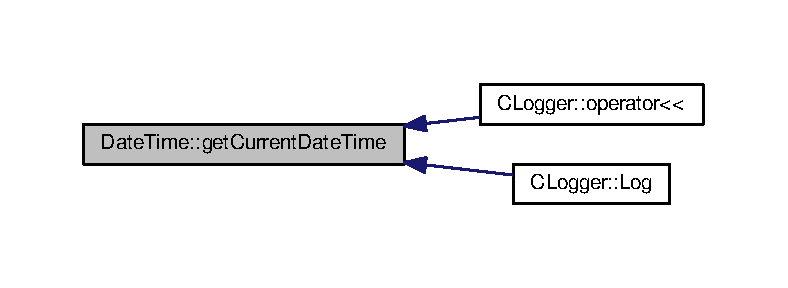
\includegraphics[width=350pt]{d0/d9c/namespaceDateTime_a7d1e8972f688ff552761398f0f75293b_icgraph}
\end{center}
\end{figure}



\chapter{Class Documentation}
\hypertarget{classCLogger}{\section{C\-Logger Class Reference}
\label{classCLogger}\index{C\-Logger@{C\-Logger}}
}


\-: It is a singleton Logger class Can we use in multithreading This class is used for logging the erro, warning or information. T\-O Do\-: Need to leverage for verbositiy level.  




{\ttfamily \#include $<$C\-Logger.\-h$>$}



Collaboration diagram for C\-Logger\-:
\nopagebreak
\begin{figure}[H]
\begin{center}
\leavevmode
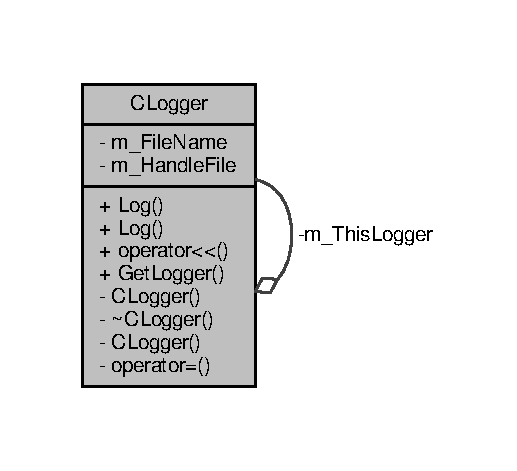
\includegraphics[width=248pt]{d9/dc8/classCLogger__coll__graph}
\end{center}
\end{figure}
\subsection*{Public Member Functions}
\begin{DoxyCompactItemize}
\item 
void \hyperlink{classCLogger_a7f66da116762cb9881af0591eda3e31b}{Log} (const std\-::string \&message)
\item 
void \hyperlink{classCLogger_a9d73d89d06a71ceb1ede9e97da2ebc4d}{Log} (const char $\ast$format,...)
\item 
\hyperlink{classCLogger}{C\-Logger} \& \hyperlink{classCLogger_a4ff21ad853c1aa9ffb5f80291b1977e3}{operator$<$$<$} (const std\-::string \&message)
\end{DoxyCompactItemize}
\subsection*{Static Public Member Functions}
\begin{DoxyCompactItemize}
\item 
static \hyperlink{classCLogger}{C\-Logger} $\ast$ \hyperlink{classCLogger_a9b863cc897927485856833316b2dcffc}{Get\-Logger} ()
\end{DoxyCompactItemize}
\subsection*{Private Member Functions}
\begin{DoxyCompactItemize}
\item 
\hyperlink{classCLogger_a9bee05627064da478ba32af360b8ef19}{C\-Logger} ()
\item 
\hyperlink{classCLogger_ab7006486dce8452e8098c12c3f44c34b}{$\sim$\-C\-Logger} ()
\item 
\hyperlink{classCLogger_ab0ff4aa1fc89d47f7bf4ae6def75d188}{C\-Logger} (const \hyperlink{classCLogger}{C\-Logger} \&)
\item 
\hyperlink{classCLogger}{C\-Logger} \& \hyperlink{classCLogger_adaa3052d7bf54fa8ca0b1b4cc0b95d10}{operator=} (const \hyperlink{classCLogger}{C\-Logger} \&)
\end{DoxyCompactItemize}
\subsection*{Static Private Attributes}
\begin{DoxyCompactItemize}
\item 
static const std\-::string \hyperlink{classCLogger_acdc0bf7adf906120da7dfa947e8de31c}{m\-\_\-\-File\-Name} =\char`\"{}/tmp/logging.\-txt\char`\"{}
\item 
static ofstream \hyperlink{classCLogger_af53cc92a313208f98e82e12c07c42955}{m\-\_\-\-Handle\-File}
\item 
static \hyperlink{classCLogger}{C\-Logger} $\ast$ \hyperlink{classCLogger_aff23c89f945de060b7679e01143bedc1}{m\-\_\-\-This\-Logger} = N\-U\-L\-L
\end{DoxyCompactItemize}


\subsection{Detailed Description}
\-: It is a singleton Logger class Can we use in multithreading This class is used for logging the erro, warning or information. T\-O Do\-: Need to leverage for verbositiy level. 

Definition at line 13 of file C\-Logger.\-h.



\subsection{Constructor \& Destructor Documentation}
\hypertarget{classCLogger_a9bee05627064da478ba32af360b8ef19}{\index{C\-Logger@{C\-Logger}!C\-Logger@{C\-Logger}}
\index{C\-Logger@{C\-Logger}!CLogger@{C\-Logger}}
\subsubsection[{C\-Logger}]{\setlength{\rightskip}{0pt plus 5cm}C\-Logger\-::\-C\-Logger (
\begin{DoxyParamCaption}
{}
\end{DoxyParamCaption}
)\hspace{0.3cm}{\ttfamily [inline]}, {\ttfamily [private]}}}\label{classCLogger_a9bee05627064da478ba32af360b8ef19}


Definition at line 20 of file C\-Logger.\-h.



Here is the caller graph for this function\-:
\nopagebreak
\begin{figure}[H]
\begin{center}
\leavevmode
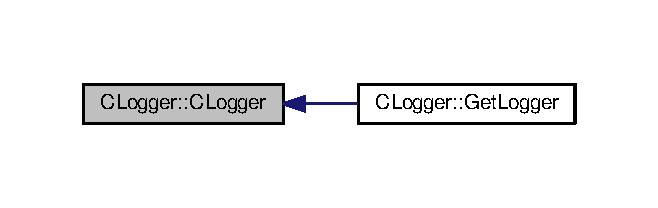
\includegraphics[width=316pt]{d4/dbe/classCLogger_a9bee05627064da478ba32af360b8ef19_icgraph}
\end{center}
\end{figure}


\hypertarget{classCLogger_ab7006486dce8452e8098c12c3f44c34b}{\index{C\-Logger@{C\-Logger}!$\sim$\-C\-Logger@{$\sim$\-C\-Logger}}
\index{$\sim$\-C\-Logger@{$\sim$\-C\-Logger}!CLogger@{C\-Logger}}
\subsubsection[{$\sim$\-C\-Logger}]{\setlength{\rightskip}{0pt plus 5cm}C\-Logger\-::$\sim$\-C\-Logger (
\begin{DoxyParamCaption}
{}
\end{DoxyParamCaption}
)\hspace{0.3cm}{\ttfamily [inline]}, {\ttfamily [private]}}}\label{classCLogger_ab7006486dce8452e8098c12c3f44c34b}


Definition at line 21 of file C\-Logger.\-h.

\hypertarget{classCLogger_ab0ff4aa1fc89d47f7bf4ae6def75d188}{\index{C\-Logger@{C\-Logger}!C\-Logger@{C\-Logger}}
\index{C\-Logger@{C\-Logger}!CLogger@{C\-Logger}}
\subsubsection[{C\-Logger}]{\setlength{\rightskip}{0pt plus 5cm}C\-Logger\-::\-C\-Logger (
\begin{DoxyParamCaption}
\item[{const {\bf C\-Logger} \&}]{}
\end{DoxyParamCaption}
)\hspace{0.3cm}{\ttfamily [inline]}, {\ttfamily [private]}}}\label{classCLogger_ab0ff4aa1fc89d47f7bf4ae6def75d188}


Definition at line 22 of file C\-Logger.\-h.



\subsection{Member Function Documentation}
\hypertarget{classCLogger_a9b863cc897927485856833316b2dcffc}{\index{C\-Logger@{C\-Logger}!Get\-Logger@{Get\-Logger}}
\index{Get\-Logger@{Get\-Logger}!CLogger@{C\-Logger}}
\subsubsection[{Get\-Logger}]{\setlength{\rightskip}{0pt plus 5cm}{\bf C\-Logger} $\ast$ C\-Logger\-::\-Get\-Logger (
\begin{DoxyParamCaption}
{}
\end{DoxyParamCaption}
)\hspace{0.3cm}{\ttfamily [static]}}}\label{classCLogger_a9b863cc897927485856833316b2dcffc}


Definition at line 10 of file C\-Logger.\-cpp.



Here is the call graph for this function\-:
\nopagebreak
\begin{figure}[H]
\begin{center}
\leavevmode
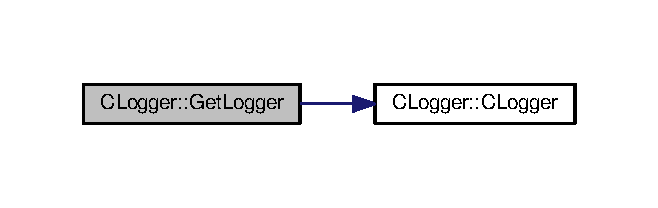
\includegraphics[width=316pt]{d4/dbe/classCLogger_a9b863cc897927485856833316b2dcffc_cgraph}
\end{center}
\end{figure}


\hypertarget{classCLogger_a7f66da116762cb9881af0591eda3e31b}{\index{C\-Logger@{C\-Logger}!Log@{Log}}
\index{Log@{Log}!CLogger@{C\-Logger}}
\subsubsection[{Log}]{\setlength{\rightskip}{0pt plus 5cm}void C\-Logger\-::\-Log (
\begin{DoxyParamCaption}
\item[{const std\-::string \&}]{message}
\end{DoxyParamCaption}
)}}\label{classCLogger_a7f66da116762cb9881af0591eda3e31b}


Definition at line 25 of file C\-Logger.\-cpp.



Here is the call graph for this function\-:
\nopagebreak
\begin{figure}[H]
\begin{center}
\leavevmode
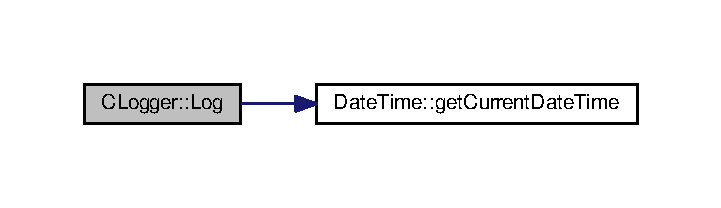
\includegraphics[width=346pt]{d4/dbe/classCLogger_a7f66da116762cb9881af0591eda3e31b_cgraph}
\end{center}
\end{figure}


\hypertarget{classCLogger_a9d73d89d06a71ceb1ede9e97da2ebc4d}{\index{C\-Logger@{C\-Logger}!Log@{Log}}
\index{Log@{Log}!CLogger@{C\-Logger}}
\subsubsection[{Log}]{\setlength{\rightskip}{0pt plus 5cm}void C\-Logger\-::\-Log (
\begin{DoxyParamCaption}
\item[{const char $\ast$}]{format, }
\item[{}]{...}
\end{DoxyParamCaption}
)}}\label{classCLogger_a9d73d89d06a71ceb1ede9e97da2ebc4d}


Definition at line 33 of file C\-Logger.\-cpp.



Here is the call graph for this function\-:
\nopagebreak
\begin{figure}[H]
\begin{center}
\leavevmode
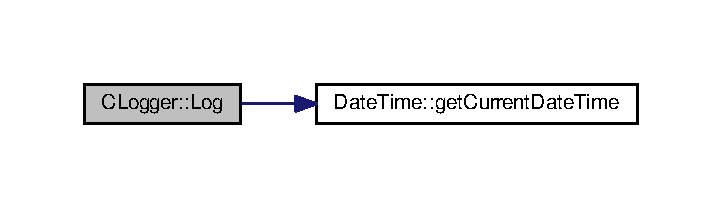
\includegraphics[width=346pt]{d4/dbe/classCLogger_a9d73d89d06a71ceb1ede9e97da2ebc4d_cgraph}
\end{center}
\end{figure}


\hypertarget{classCLogger_a4ff21ad853c1aa9ffb5f80291b1977e3}{\index{C\-Logger@{C\-Logger}!operator$<$$<$@{operator$<$$<$}}
\index{operator$<$$<$@{operator$<$$<$}!CLogger@{C\-Logger}}
\subsubsection[{operator$<$$<$}]{\setlength{\rightskip}{0pt plus 5cm}{\bf C\-Logger} \& C\-Logger\-::operator$<$$<$ (
\begin{DoxyParamCaption}
\item[{const std\-::string \&}]{message}
\end{DoxyParamCaption}
)}}\label{classCLogger_a4ff21ad853c1aa9ffb5f80291b1977e3}


Definition at line 17 of file C\-Logger.\-cpp.



Here is the call graph for this function\-:
\nopagebreak
\begin{figure}[H]
\begin{center}
\leavevmode
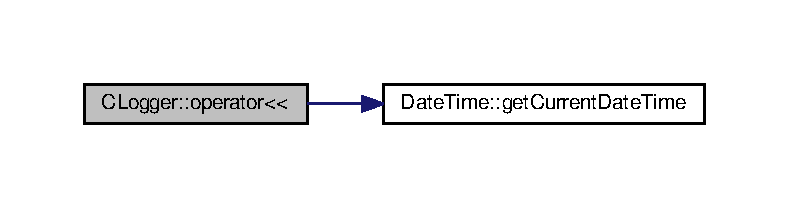
\includegraphics[width=350pt]{d4/dbe/classCLogger_a4ff21ad853c1aa9ffb5f80291b1977e3_cgraph}
\end{center}
\end{figure}


\hypertarget{classCLogger_adaa3052d7bf54fa8ca0b1b4cc0b95d10}{\index{C\-Logger@{C\-Logger}!operator=@{operator=}}
\index{operator=@{operator=}!CLogger@{C\-Logger}}
\subsubsection[{operator=}]{\setlength{\rightskip}{0pt plus 5cm}{\bf C\-Logger}\& C\-Logger\-::operator= (
\begin{DoxyParamCaption}
\item[{const {\bf C\-Logger} \&}]{}
\end{DoxyParamCaption}
)\hspace{0.3cm}{\ttfamily [inline]}, {\ttfamily [private]}}}\label{classCLogger_adaa3052d7bf54fa8ca0b1b4cc0b95d10}


Definition at line 23 of file C\-Logger.\-h.



\subsection{Member Data Documentation}
\hypertarget{classCLogger_acdc0bf7adf906120da7dfa947e8de31c}{\index{C\-Logger@{C\-Logger}!m\-\_\-\-File\-Name@{m\-\_\-\-File\-Name}}
\index{m\-\_\-\-File\-Name@{m\-\_\-\-File\-Name}!CLogger@{C\-Logger}}
\subsubsection[{m\-\_\-\-File\-Name}]{\setlength{\rightskip}{0pt plus 5cm}const std\-::string C\-Logger\-::m\-\_\-\-File\-Name =\char`\"{}/tmp/logging.\-txt\char`\"{}\hspace{0.3cm}{\ttfamily [static]}, {\ttfamily [private]}}}\label{classCLogger_acdc0bf7adf906120da7dfa947e8de31c}


Definition at line 25 of file C\-Logger.\-h.

\hypertarget{classCLogger_af53cc92a313208f98e82e12c07c42955}{\index{C\-Logger@{C\-Logger}!m\-\_\-\-Handle\-File@{m\-\_\-\-Handle\-File}}
\index{m\-\_\-\-Handle\-File@{m\-\_\-\-Handle\-File}!CLogger@{C\-Logger}}
\subsubsection[{m\-\_\-\-Handle\-File}]{\setlength{\rightskip}{0pt plus 5cm}ofstream C\-Logger\-::m\-\_\-\-Handle\-File\hspace{0.3cm}{\ttfamily [static]}, {\ttfamily [private]}}}\label{classCLogger_af53cc92a313208f98e82e12c07c42955}


Definition at line 26 of file C\-Logger.\-h.

\hypertarget{classCLogger_aff23c89f945de060b7679e01143bedc1}{\index{C\-Logger@{C\-Logger}!m\-\_\-\-This\-Logger@{m\-\_\-\-This\-Logger}}
\index{m\-\_\-\-This\-Logger@{m\-\_\-\-This\-Logger}!CLogger@{C\-Logger}}
\subsubsection[{m\-\_\-\-This\-Logger}]{\setlength{\rightskip}{0pt plus 5cm}{\bf C\-Logger} $\ast$ C\-Logger\-::m\-\_\-\-This\-Logger = N\-U\-L\-L\hspace{0.3cm}{\ttfamily [static]}, {\ttfamily [private]}}}\label{classCLogger_aff23c89f945de060b7679e01143bedc1}


Definition at line 27 of file C\-Logger.\-h.



The documentation for this class was generated from the following files\-:\begin{DoxyCompactItemize}
\item 
logging/include/\hyperlink{CLogger_8h}{C\-Logger.\-h}\item 
logging/source/\hyperlink{CLogger_8cpp}{C\-Logger.\-cpp}\end{DoxyCompactItemize}

\hypertarget{classCLoggerException}{\section{C\-Logger\-Exception Class Reference}
\label{classCLoggerException}\index{C\-Logger\-Exception@{C\-Logger\-Exception}}
}


{\ttfamily \#include $<$C\-Logger\-Exception.\-h$>$}



Inheritance diagram for C\-Logger\-Exception\-:
\nopagebreak
\begin{figure}[H]
\begin{center}
\leavevmode
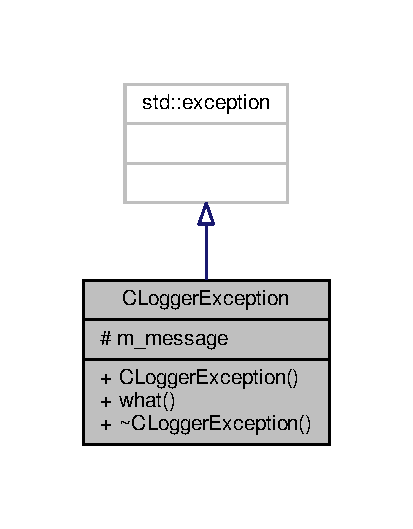
\includegraphics[width=198pt]{dd/d50/classCLoggerException__inherit__graph}
\end{center}
\end{figure}


Collaboration diagram for C\-Logger\-Exception\-:
\nopagebreak
\begin{figure}[H]
\begin{center}
\leavevmode
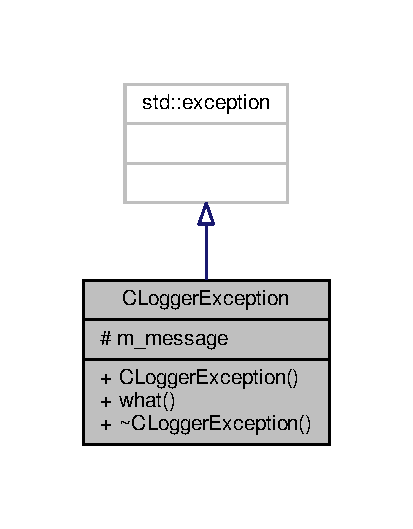
\includegraphics[width=198pt]{d2/d86/classCLoggerException__coll__graph}
\end{center}
\end{figure}
\subsection*{Public Member Functions}
\begin{DoxyCompactItemize}
\item 
\hyperlink{classCLoggerException_ae14f1a264ddc7181ff19e36e3f9cd69d}{C\-Logger\-Exception} (const std\-::string \&message, bool sye\-Error=false)  throw ()
\item 
const char $\ast$ \hyperlink{classCLoggerException_a0f91ad11b6665d3348a8eb66d5bcfe4e}{what} () const   throw ()
\item 
virtual \hyperlink{classCLoggerException_a2604baa2d3fc6f13c83d5c606fd99941}{$\sim$\-C\-Logger\-Exception} ()  throw ()
\end{DoxyCompactItemize}
\subsection*{Protected Attributes}
\begin{DoxyCompactItemize}
\item 
std\-::string \hyperlink{classCLoggerException_a4bbe88a45b230e4f6ca3246999c8348a}{m\-\_\-message}
\end{DoxyCompactItemize}


\subsection{Detailed Description}


Definition at line 4 of file C\-Logger\-Exception.\-h.



\subsection{Constructor \& Destructor Documentation}
\hypertarget{classCLoggerException_ae14f1a264ddc7181ff19e36e3f9cd69d}{\index{C\-Logger\-Exception@{C\-Logger\-Exception}!C\-Logger\-Exception@{C\-Logger\-Exception}}
\index{C\-Logger\-Exception@{C\-Logger\-Exception}!CLoggerException@{C\-Logger\-Exception}}
\subsubsection[{C\-Logger\-Exception}]{\setlength{\rightskip}{0pt plus 5cm}C\-Logger\-Exception\-::\-C\-Logger\-Exception (
\begin{DoxyParamCaption}
\item[{const std\-::string \&}]{message, }
\item[{bool}]{sye\-Error = {\ttfamily false}}
\end{DoxyParamCaption}
) throw  ) }}\label{classCLoggerException_ae14f1a264ddc7181ff19e36e3f9cd69d}


Definition at line 15 of file C\-Logger\-Exception.\-cpp.



Here is the call graph for this function\-:
\nopagebreak
\begin{figure}[H]
\begin{center}
\leavevmode
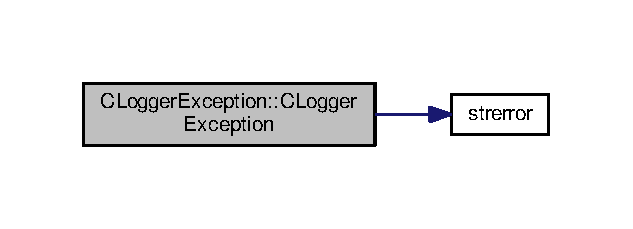
\includegraphics[width=304pt]{d9/de1/classCLoggerException_ae14f1a264ddc7181ff19e36e3f9cd69d_cgraph}
\end{center}
\end{figure}


\hypertarget{classCLoggerException_a2604baa2d3fc6f13c83d5c606fd99941}{\index{C\-Logger\-Exception@{C\-Logger\-Exception}!$\sim$\-C\-Logger\-Exception@{$\sim$\-C\-Logger\-Exception}}
\index{$\sim$\-C\-Logger\-Exception@{$\sim$\-C\-Logger\-Exception}!CLoggerException@{C\-Logger\-Exception}}
\subsubsection[{$\sim$\-C\-Logger\-Exception}]{\setlength{\rightskip}{0pt plus 5cm}C\-Logger\-Exception\-::$\sim$\-C\-Logger\-Exception (
\begin{DoxyParamCaption}
{}
\end{DoxyParamCaption}
) throw  ) \hspace{0.3cm}{\ttfamily [virtual]}}}\label{classCLoggerException_a2604baa2d3fc6f13c83d5c606fd99941}


Definition at line 30 of file C\-Logger\-Exception.\-cpp.



\subsection{Member Function Documentation}
\hypertarget{classCLoggerException_a0f91ad11b6665d3348a8eb66d5bcfe4e}{\index{C\-Logger\-Exception@{C\-Logger\-Exception}!what@{what}}
\index{what@{what}!CLoggerException@{C\-Logger\-Exception}}
\subsubsection[{what}]{\setlength{\rightskip}{0pt plus 5cm}const char $\ast$ C\-Logger\-Exception\-::what (
\begin{DoxyParamCaption}
{}
\end{DoxyParamCaption}
) const throw  ) }}\label{classCLoggerException_a0f91ad11b6665d3348a8eb66d5bcfe4e}


Definition at line 25 of file C\-Logger\-Exception.\-cpp.



\subsection{Member Data Documentation}
\hypertarget{classCLoggerException_a4bbe88a45b230e4f6ca3246999c8348a}{\index{C\-Logger\-Exception@{C\-Logger\-Exception}!m\-\_\-message@{m\-\_\-message}}
\index{m\-\_\-message@{m\-\_\-message}!CLoggerException@{C\-Logger\-Exception}}
\subsubsection[{m\-\_\-message}]{\setlength{\rightskip}{0pt plus 5cm}std\-::string C\-Logger\-Exception\-::m\-\_\-message\hspace{0.3cm}{\ttfamily [protected]}}}\label{classCLoggerException_a4bbe88a45b230e4f6ca3246999c8348a}


Definition at line 10 of file C\-Logger\-Exception.\-h.



The documentation for this class was generated from the following files\-:\begin{DoxyCompactItemize}
\item 
logging/include/\hyperlink{CLoggerException_8h}{C\-Logger\-Exception.\-h}\item 
logging/source/\hyperlink{CLoggerException_8cpp}{C\-Logger\-Exception.\-cpp}\end{DoxyCompactItemize}

\hypertarget{classCMutex}{\section{C\-Mutex Class Reference}
\label{classCMutex}\index{C\-Mutex@{C\-Mutex}}
}


\-: Mutex class to achieve synchronization  




{\ttfamily \#include $<$C\-Mutex.\-h$>$}



Collaboration diagram for C\-Mutex\-:
\nopagebreak
\begin{figure}[H]
\begin{center}
\leavevmode
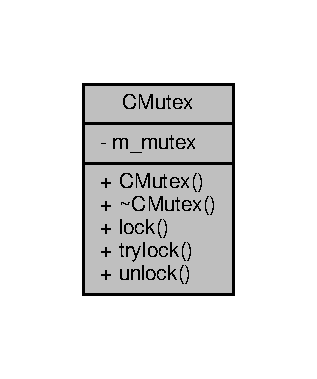
\includegraphics[width=152pt]{d4/db7/classCMutex__coll__graph}
\end{center}
\end{figure}
\subsection*{Public Member Functions}
\begin{DoxyCompactItemize}
\item 
\hyperlink{classCMutex_a9c050f1451600e8bc35c4c80f6533800}{C\-Mutex} ()
\item 
virtual \hyperlink{classCMutex_a59780a1a2a0e85377886c08e91817048}{$\sim$\-C\-Mutex} ()
\item 
int \hyperlink{classCMutex_a9ef2455d929bb4bd9dd458a35c8bc9a6}{lock} ()
\item 
int \hyperlink{classCMutex_a6d7acb0de2dc55a1fc765055772c132d}{trylock} ()
\item 
int \hyperlink{classCMutex_a98da3b28764101df37a6f3935066a149}{unlock} ()
\end{DoxyCompactItemize}
\subsection*{Private Attributes}
\begin{DoxyCompactItemize}
\item 
pthread\-\_\-mutex\-\_\-t \hyperlink{classCMutex_a0e47869fa098e329321e674647732b4d}{m\-\_\-mutex}
\end{DoxyCompactItemize}


\subsection{Detailed Description}
\-: Mutex class to achieve synchronization 

Definition at line 9 of file C\-Mutex.\-h.



\subsection{Constructor \& Destructor Documentation}
\hypertarget{classCMutex_a9c050f1451600e8bc35c4c80f6533800}{\index{C\-Mutex@{C\-Mutex}!C\-Mutex@{C\-Mutex}}
\index{C\-Mutex@{C\-Mutex}!CMutex@{C\-Mutex}}
\subsubsection[{C\-Mutex}]{\setlength{\rightskip}{0pt plus 5cm}C\-Mutex\-::\-C\-Mutex (
\begin{DoxyParamCaption}
{}
\end{DoxyParamCaption}
)\hspace{0.3cm}{\ttfamily [inline]}}}\label{classCMutex_a9c050f1451600e8bc35c4c80f6533800}


Definition at line 15 of file C\-Mutex.\-h.

\hypertarget{classCMutex_a59780a1a2a0e85377886c08e91817048}{\index{C\-Mutex@{C\-Mutex}!$\sim$\-C\-Mutex@{$\sim$\-C\-Mutex}}
\index{$\sim$\-C\-Mutex@{$\sim$\-C\-Mutex}!CMutex@{C\-Mutex}}
\subsubsection[{$\sim$\-C\-Mutex}]{\setlength{\rightskip}{0pt plus 5cm}virtual C\-Mutex\-::$\sim$\-C\-Mutex (
\begin{DoxyParamCaption}
{}
\end{DoxyParamCaption}
)\hspace{0.3cm}{\ttfamily [inline]}, {\ttfamily [virtual]}}}\label{classCMutex_a59780a1a2a0e85377886c08e91817048}


Definition at line 16 of file C\-Mutex.\-h.



\subsection{Member Function Documentation}
\hypertarget{classCMutex_a9ef2455d929bb4bd9dd458a35c8bc9a6}{\index{C\-Mutex@{C\-Mutex}!lock@{lock}}
\index{lock@{lock}!CMutex@{C\-Mutex}}
\subsubsection[{lock}]{\setlength{\rightskip}{0pt plus 5cm}int C\-Mutex\-::lock (
\begin{DoxyParamCaption}
{}
\end{DoxyParamCaption}
)\hspace{0.3cm}{\ttfamily [inline]}}}\label{classCMutex_a9ef2455d929bb4bd9dd458a35c8bc9a6}


Definition at line 21 of file C\-Mutex.\-h.

\hypertarget{classCMutex_a6d7acb0de2dc55a1fc765055772c132d}{\index{C\-Mutex@{C\-Mutex}!trylock@{trylock}}
\index{trylock@{trylock}!CMutex@{C\-Mutex}}
\subsubsection[{trylock}]{\setlength{\rightskip}{0pt plus 5cm}int C\-Mutex\-::trylock (
\begin{DoxyParamCaption}
{}
\end{DoxyParamCaption}
)\hspace{0.3cm}{\ttfamily [inline]}}}\label{classCMutex_a6d7acb0de2dc55a1fc765055772c132d}


Definition at line 22 of file C\-Mutex.\-h.

\hypertarget{classCMutex_a98da3b28764101df37a6f3935066a149}{\index{C\-Mutex@{C\-Mutex}!unlock@{unlock}}
\index{unlock@{unlock}!CMutex@{C\-Mutex}}
\subsubsection[{unlock}]{\setlength{\rightskip}{0pt plus 5cm}int C\-Mutex\-::unlock (
\begin{DoxyParamCaption}
{}
\end{DoxyParamCaption}
)\hspace{0.3cm}{\ttfamily [inline]}}}\label{classCMutex_a98da3b28764101df37a6f3935066a149}


Definition at line 23 of file C\-Mutex.\-h.



\subsection{Member Data Documentation}
\hypertarget{classCMutex_a0e47869fa098e329321e674647732b4d}{\index{C\-Mutex@{C\-Mutex}!m\-\_\-mutex@{m\-\_\-mutex}}
\index{m\-\_\-mutex@{m\-\_\-mutex}!CMutex@{C\-Mutex}}
\subsubsection[{m\-\_\-mutex}]{\setlength{\rightskip}{0pt plus 5cm}pthread\-\_\-mutex\-\_\-t C\-Mutex\-::m\-\_\-mutex\hspace{0.3cm}{\ttfamily [private]}}}\label{classCMutex_a0e47869fa098e329321e674647732b4d}


Definition at line 11 of file C\-Mutex.\-h.



The documentation for this class was generated from the following file\-:\begin{DoxyCompactItemize}
\item 
logging/include/\hyperlink{CMutex_8h}{C\-Mutex.\-h}\end{DoxyCompactItemize}

\chapter{File Documentation}
\hypertarget{ClientServer_2client_2Makefile}{\section{Client\-Server/client/\-Makefile File Reference}
\label{ClientServer_2client_2Makefile}\index{Client\-Server/client/\-Makefile@{Client\-Server/client/\-Makefile}}
}
\subsection*{Macros}
\begin{DoxyCompactItemize}
\item 
\#define \hyperlink{ClientServer_2client_2Makefile_a09c6b60bb7451f9136e25140ffdff6bd}{the}~C compiler to use
\item 
\#define \hyperlink{ClientServer_2client_2Makefile_a6120b6f1abea66c8ede7b300a66d4cc0}{any}~compile-\/time flags
\item 
\#define \hyperlink{ClientServer_2client_2Makefile_a6120b6f1abea66c8ede7b300a66d4cc0}{any}~directories containing header files other than /usr/include
\item 
\#define \hyperlink{ClientServer_2client_2Makefile_a1f477410360bd4832116581b9934ab71}{library}~paths in addition to /usr/lib
\end{DoxyCompactItemize}


\subsection{Macro Definition Documentation}
\hypertarget{ClientServer_2client_2Makefile_a6120b6f1abea66c8ede7b300a66d4cc0}{\index{Client\-Server/client/\-Makefile@{Client\-Server/client/\-Makefile}!any@{any}}
\index{any@{any}!ClientServer/client/Makefile@{Client\-Server/client/\-Makefile}}
\subsubsection[{any}]{\setlength{\rightskip}{0pt plus 5cm}\#define any~compile-\/time flags}}\label{ClientServer_2client_2Makefile_a6120b6f1abea66c8ede7b300a66d4cc0}
\hypertarget{ClientServer_2client_2Makefile_a6120b6f1abea66c8ede7b300a66d4cc0}{\index{Client\-Server/client/\-Makefile@{Client\-Server/client/\-Makefile}!any@{any}}
\index{any@{any}!ClientServer/client/Makefile@{Client\-Server/client/\-Makefile}}
\subsubsection[{any}]{\setlength{\rightskip}{0pt plus 5cm}\#define any~directories containing header files other than /usr/include}}\label{ClientServer_2client_2Makefile_a6120b6f1abea66c8ede7b300a66d4cc0}
\hypertarget{ClientServer_2client_2Makefile_a1f477410360bd4832116581b9934ab71}{\index{Client\-Server/client/\-Makefile@{Client\-Server/client/\-Makefile}!library@{library}}
\index{library@{library}!ClientServer/client/Makefile@{Client\-Server/client/\-Makefile}}
\subsubsection[{library}]{\setlength{\rightskip}{0pt plus 5cm}\#define library~paths in addition to /usr/lib}}\label{ClientServer_2client_2Makefile_a1f477410360bd4832116581b9934ab71}
\hypertarget{ClientServer_2client_2Makefile_a09c6b60bb7451f9136e25140ffdff6bd}{\index{Client\-Server/client/\-Makefile@{Client\-Server/client/\-Makefile}!the@{the}}
\index{the@{the}!ClientServer/client/Makefile@{Client\-Server/client/\-Makefile}}
\subsubsection[{the}]{\setlength{\rightskip}{0pt plus 5cm}\#define the~C compiler to use}}\label{ClientServer_2client_2Makefile_a09c6b60bb7451f9136e25140ffdff6bd}


Definition at line 10 of file Makefile.


\hypertarget{ClientServer_2Makefile}{\section{Client\-Server/\-Makefile File Reference}
\label{ClientServer_2Makefile}\index{Client\-Server/\-Makefile@{Client\-Server/\-Makefile}}
}
\subsection*{Functions}
\begin{DoxyCompactItemize}
\item 
\hyperlink{ClientServer_2Makefile_a54d2d882a8cc61f85bf978b5e4317ab1}{do} (M\-A\-K\-E)-\/C \$\$dir-\/f Makefile \$@
\end{DoxyCompactItemize}
\subsection*{Variables}
\begin{DoxyCompactItemize}
\item 
\hyperlink{ClientServer_2Makefile_a290c239123caef8485b75428c4acc522}{S\-U\-B\-D\-I\-R\-S}
\end{DoxyCompactItemize}


\subsection{Function Documentation}
\hypertarget{ClientServer_2Makefile_a54d2d882a8cc61f85bf978b5e4317ab1}{\index{Client\-Server/\-Makefile@{Client\-Server/\-Makefile}!do@{do}}
\index{do@{do}!ClientServer/Makefile@{Client\-Server/\-Makefile}}
\subsubsection[{do}]{\setlength{\rightskip}{0pt plus 5cm}do (
\begin{DoxyParamCaption}
\item[{M\-A\-K\-E}]{}
\end{DoxyParamCaption}
)}}\label{ClientServer_2Makefile_a54d2d882a8cc61f85bf978b5e4317ab1}


\subsection{Variable Documentation}
\hypertarget{ClientServer_2Makefile_a290c239123caef8485b75428c4acc522}{\index{Client\-Server/\-Makefile@{Client\-Server/\-Makefile}!S\-U\-B\-D\-I\-R\-S@{S\-U\-B\-D\-I\-R\-S}}
\index{S\-U\-B\-D\-I\-R\-S@{S\-U\-B\-D\-I\-R\-S}!ClientServer/Makefile@{Client\-Server/\-Makefile}}
\subsubsection[{S\-U\-B\-D\-I\-R\-S}]{\setlength{\rightskip}{0pt plus 5cm}S\-U\-B\-D\-I\-R\-S}}\label{ClientServer_2Makefile_a290c239123caef8485b75428c4acc522}
{\bfseries Initial value\-:}
\begin{DoxyCode}
= server client

.PHONY: all clean

all clean:
    \textcolor{keywordflow}{for} dir in $(\hyperlink{ClientServer_2Makefile_a290c239123caef8485b75428c4acc522}{SUBDIRS})
\end{DoxyCode}


Definition at line 1 of file Makefile.


\hypertarget{ClientServer_2server_2Makefile}{\section{Client\-Server/server/\-Makefile File Reference}
\label{ClientServer_2server_2Makefile}\index{Client\-Server/server/\-Makefile@{Client\-Server/server/\-Makefile}}
}
\subsection*{Macros}
\begin{DoxyCompactItemize}
\item 
\#define \hyperlink{ClientServer_2server_2Makefile_a09c6b60bb7451f9136e25140ffdff6bd}{the}~C compiler to use
\item 
\#define \hyperlink{ClientServer_2server_2Makefile_a6120b6f1abea66c8ede7b300a66d4cc0}{any}~compile-\/time flags
\item 
\#define \hyperlink{ClientServer_2server_2Makefile_a6120b6f1abea66c8ede7b300a66d4cc0}{any}~directories containing header files other than /usr/include
\item 
\#define \hyperlink{ClientServer_2server_2Makefile_a1f477410360bd4832116581b9934ab71}{library}~paths in addition to /usr/lib
\end{DoxyCompactItemize}


\subsection{Macro Definition Documentation}
\hypertarget{ClientServer_2server_2Makefile_a6120b6f1abea66c8ede7b300a66d4cc0}{\index{Client\-Server/server/\-Makefile@{Client\-Server/server/\-Makefile}!any@{any}}
\index{any@{any}!ClientServer/server/Makefile@{Client\-Server/server/\-Makefile}}
\subsubsection[{any}]{\setlength{\rightskip}{0pt plus 5cm}\#define any~compile-\/time flags}}\label{ClientServer_2server_2Makefile_a6120b6f1abea66c8ede7b300a66d4cc0}
\hypertarget{ClientServer_2server_2Makefile_a6120b6f1abea66c8ede7b300a66d4cc0}{\index{Client\-Server/server/\-Makefile@{Client\-Server/server/\-Makefile}!any@{any}}
\index{any@{any}!ClientServer/server/Makefile@{Client\-Server/server/\-Makefile}}
\subsubsection[{any}]{\setlength{\rightskip}{0pt plus 5cm}\#define any~directories containing header files other than /usr/include}}\label{ClientServer_2server_2Makefile_a6120b6f1abea66c8ede7b300a66d4cc0}
\hypertarget{ClientServer_2server_2Makefile_a1f477410360bd4832116581b9934ab71}{\index{Client\-Server/server/\-Makefile@{Client\-Server/server/\-Makefile}!library@{library}}
\index{library@{library}!ClientServer/server/Makefile@{Client\-Server/server/\-Makefile}}
\subsubsection[{library}]{\setlength{\rightskip}{0pt plus 5cm}\#define library~paths in addition to /usr/lib}}\label{ClientServer_2server_2Makefile_a1f477410360bd4832116581b9934ab71}
\hypertarget{ClientServer_2server_2Makefile_a09c6b60bb7451f9136e25140ffdff6bd}{\index{Client\-Server/server/\-Makefile@{Client\-Server/server/\-Makefile}!the@{the}}
\index{the@{the}!ClientServer/server/Makefile@{Client\-Server/server/\-Makefile}}
\subsubsection[{the}]{\setlength{\rightskip}{0pt plus 5cm}\#define the~C compiler to use}}\label{ClientServer_2server_2Makefile_a09c6b60bb7451f9136e25140ffdff6bd}


Definition at line 10 of file Makefile.


\hypertarget{common_2Makefile}{\section{common/\-Makefile File Reference}
\label{common_2Makefile}\index{common/\-Makefile@{common/\-Makefile}}
}

\hypertarget{logging_2Makefile}{\section{logging/\-Makefile File Reference}
\label{logging_2Makefile}\index{logging/\-Makefile@{logging/\-Makefile}}
}

\hypertarget{Makefile}{\section{Makefile File Reference}
\label{Makefile}\index{Makefile@{Makefile}}
}
\subsection*{Functions}
\begin{DoxyCompactItemize}
\item 
\hyperlink{Makefile_a54d2d882a8cc61f85bf978b5e4317ab1}{do} (M\-A\-K\-E)-\/C \$\$dir-\/f Makefile \$@
\end{DoxyCompactItemize}
\subsection*{Variables}
\begin{DoxyCompactItemize}
\item 
\hyperlink{Makefile_a290c239123caef8485b75428c4acc522}{S\-U\-B\-D\-I\-R\-S}
\end{DoxyCompactItemize}


\subsection{Function Documentation}
\hypertarget{Makefile_a54d2d882a8cc61f85bf978b5e4317ab1}{\index{Makefile@{Makefile}!do@{do}}
\index{do@{do}!Makefile@{Makefile}}
\subsubsection[{do}]{\setlength{\rightskip}{0pt plus 5cm}do (
\begin{DoxyParamCaption}
\item[{M\-A\-K\-E}]{}
\end{DoxyParamCaption}
)}}\label{Makefile_a54d2d882a8cc61f85bf978b5e4317ab1}


\subsection{Variable Documentation}
\hypertarget{Makefile_a290c239123caef8485b75428c4acc522}{\index{Makefile@{Makefile}!S\-U\-B\-D\-I\-R\-S@{S\-U\-B\-D\-I\-R\-S}}
\index{S\-U\-B\-D\-I\-R\-S@{S\-U\-B\-D\-I\-R\-S}!Makefile@{Makefile}}
\subsubsection[{S\-U\-B\-D\-I\-R\-S}]{\setlength{\rightskip}{0pt plus 5cm}S\-U\-B\-D\-I\-R\-S}}\label{Makefile_a290c239123caef8485b75428c4acc522}
{\bfseries Initial value\-:}
\begin{DoxyCode}
= common logging tcpSocket ClientServer

.PHONY: all clean

all clean:
    \textcolor{keywordflow}{for} dir in $(\hyperlink{ClientServer_2Makefile_a290c239123caef8485b75428c4acc522}{SUBDIRS})
\end{DoxyCode}


Definition at line 1 of file Makefile.


\hypertarget{tcpSocket_2Makefile}{\section{tcp\-Socket/\-Makefile File Reference}
\label{tcpSocket_2Makefile}\index{tcp\-Socket/\-Makefile@{tcp\-Socket/\-Makefile}}
}

\hypertarget{client_8cpp}{\section{Client\-Server/client/source/client.cpp File Reference}
\label{client_8cpp}\index{Client\-Server/client/source/client.\-cpp@{Client\-Server/client/source/client.\-cpp}}
}
{\ttfamily \#include $<$stdio.\-h$>$}\\*
{\ttfamily \#include $<$stdlib.\-h$>$}\\*
{\ttfamily \#include $<$string.\-h$>$}\\*
{\ttfamily \#include $<$unistd.\-h$>$}\\*
{\ttfamily \#include \char`\"{}inet\-\_\-socket.\-h\char`\"{}}\\*
{\ttfamily \#include \char`\"{}inet\-\_\-handle\-\_\-multiplex\-\_\-io.\-h\char`\"{}}\\*
{\ttfamily \#include \char`\"{}C\-Logger.\-h\char`\"{}}\\*
Include dependency graph for client.\-cpp\-:
\nopagebreak
\begin{figure}[H]
\begin{center}
\leavevmode
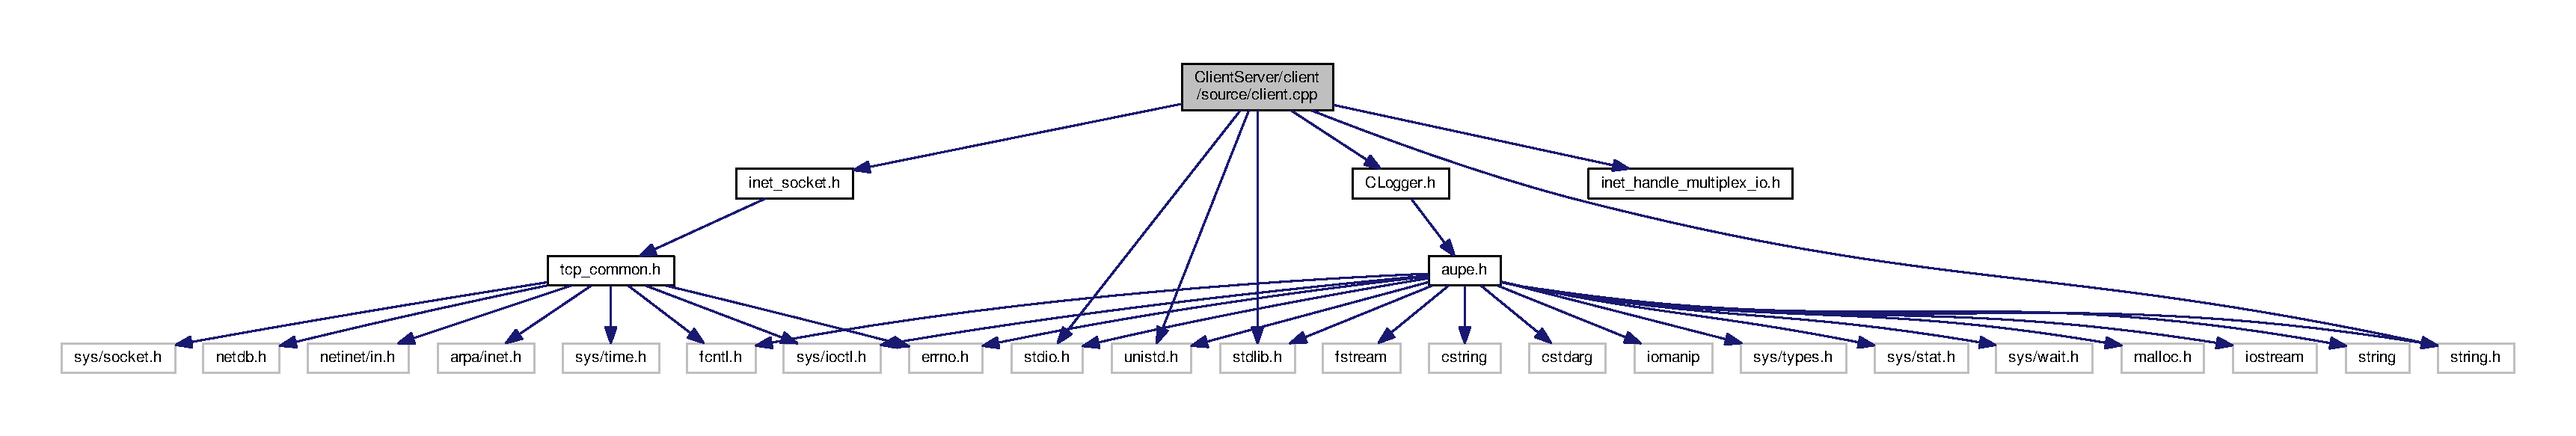
\includegraphics[width=350pt]{d0/d48/client_8cpp__incl}
\end{center}
\end{figure}
\subsection*{Macros}
\begin{DoxyCompactItemize}
\item 
\#define \hyperlink{client_8cpp_a16c16f9369be4a374a3e621f6d13bb16}{M\-A\-X\-D\-A\-T\-A\-S\-I\-Z\-E}~128
\end{DoxyCompactItemize}
\subsection*{Functions}
\begin{DoxyCompactItemize}
\item 
void \hyperlink{client_8cpp_ac17020a38607ab29ce18939d5194a32a}{func} (int sockfd)
\item 
int \hyperlink{client_8cpp_a0ddf1224851353fc92bfbff6f499fa97}{main} (int argc, char $\ast$argv\mbox{[}$\,$\mbox{]})
\end{DoxyCompactItemize}


\subsection{Macro Definition Documentation}
\hypertarget{client_8cpp_a16c16f9369be4a374a3e621f6d13bb16}{\index{client.\-cpp@{client.\-cpp}!M\-A\-X\-D\-A\-T\-A\-S\-I\-Z\-E@{M\-A\-X\-D\-A\-T\-A\-S\-I\-Z\-E}}
\index{M\-A\-X\-D\-A\-T\-A\-S\-I\-Z\-E@{M\-A\-X\-D\-A\-T\-A\-S\-I\-Z\-E}!client.cpp@{client.\-cpp}}
\subsubsection[{M\-A\-X\-D\-A\-T\-A\-S\-I\-Z\-E}]{\setlength{\rightskip}{0pt plus 5cm}\#define M\-A\-X\-D\-A\-T\-A\-S\-I\-Z\-E~128}}\label{client_8cpp_a16c16f9369be4a374a3e621f6d13bb16}


Definition at line 9 of file client.\-cpp.



\subsection{Function Documentation}
\hypertarget{client_8cpp_ac17020a38607ab29ce18939d5194a32a}{\index{client.\-cpp@{client.\-cpp}!func@{func}}
\index{func@{func}!client.cpp@{client.\-cpp}}
\subsubsection[{func}]{\setlength{\rightskip}{0pt plus 5cm}void func (
\begin{DoxyParamCaption}
\item[{int}]{sockfd}
\end{DoxyParamCaption}
)}}\label{client_8cpp_ac17020a38607ab29ce18939d5194a32a}


Definition at line 12 of file client.\-cpp.



Here is the call graph for this function\-:
\nopagebreak
\begin{figure}[H]
\begin{center}
\leavevmode
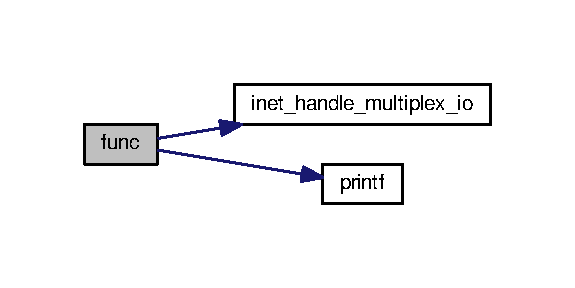
\includegraphics[width=276pt]{d9/d95/client_8cpp_ac17020a38607ab29ce18939d5194a32a_cgraph}
\end{center}
\end{figure}




Here is the caller graph for this function\-:
\nopagebreak
\begin{figure}[H]
\begin{center}
\leavevmode
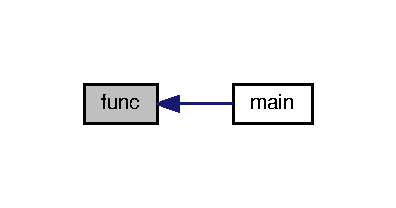
\includegraphics[width=190pt]{d9/d95/client_8cpp_ac17020a38607ab29ce18939d5194a32a_icgraph}
\end{center}
\end{figure}


\hypertarget{client_8cpp_a0ddf1224851353fc92bfbff6f499fa97}{\index{client.\-cpp@{client.\-cpp}!main@{main}}
\index{main@{main}!client.cpp@{client.\-cpp}}
\subsubsection[{main}]{\setlength{\rightskip}{0pt plus 5cm}int main (
\begin{DoxyParamCaption}
\item[{int}]{argc, }
\item[{char $\ast$}]{argv\mbox{[}$\,$\mbox{]}}
\end{DoxyParamCaption}
)}}\label{client_8cpp_a0ddf1224851353fc92bfbff6f499fa97}


Definition at line 44 of file client.\-cpp.



Here is the call graph for this function\-:
\nopagebreak
\begin{figure}[H]
\begin{center}
\leavevmode
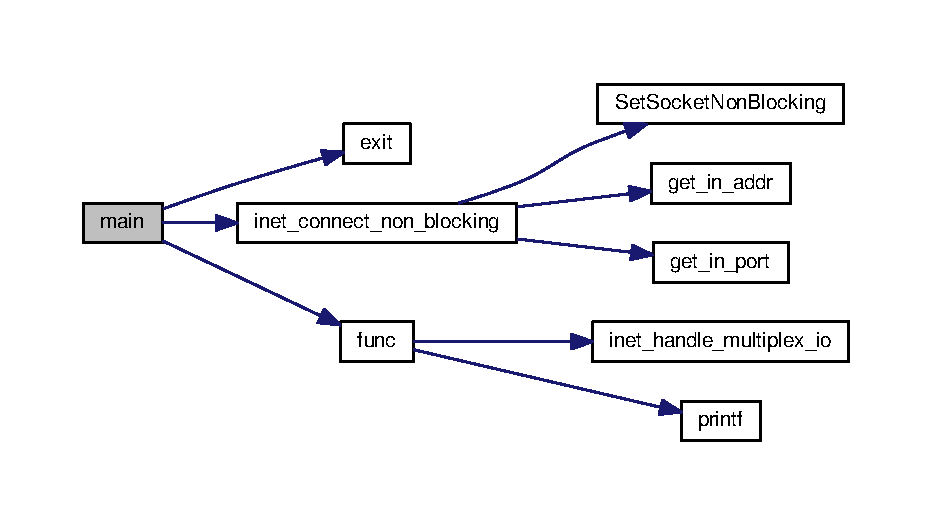
\includegraphics[width=350pt]{d9/d95/client_8cpp_a0ddf1224851353fc92bfbff6f499fa97_cgraph}
\end{center}
\end{figure}



\hypertarget{server_8cpp}{\section{Client\-Server/server/source/server.cpp File Reference}
\label{server_8cpp}\index{Client\-Server/server/source/server.\-cpp@{Client\-Server/server/source/server.\-cpp}}
}
{\ttfamily \#include \char`\"{}inet\-\_\-socket.\-h\char`\"{}}\\*
{\ttfamily \#include \char`\"{}inet\-\_\-accept.\-h\char`\"{}}\\*
{\ttfamily \#include \char`\"{}C\-Logger.\-h\char`\"{}}\\*
Include dependency graph for server.\-cpp\-:
\nopagebreak
\begin{figure}[H]
\begin{center}
\leavevmode
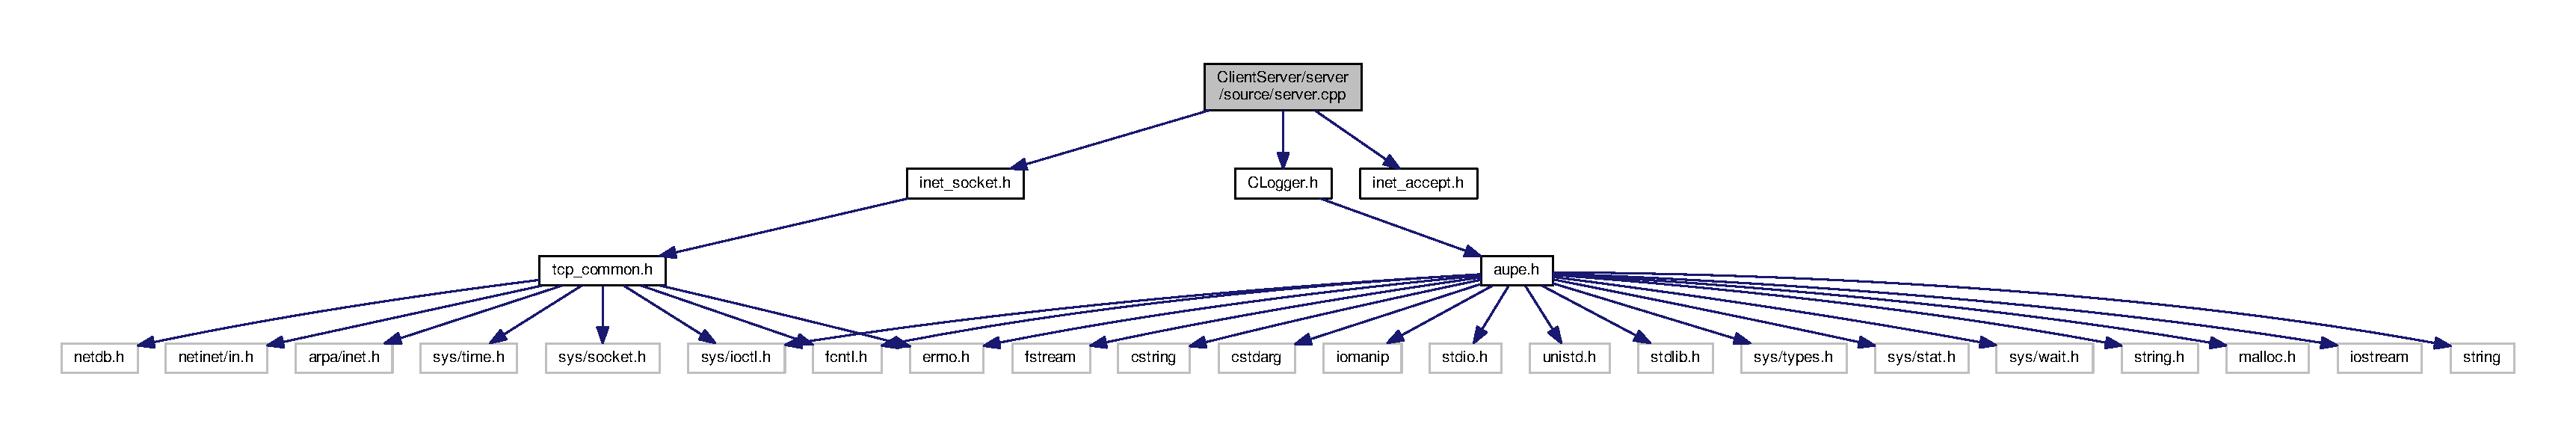
\includegraphics[width=350pt]{d4/d48/server_8cpp__incl}
\end{center}
\end{figure}
\subsection*{Macros}
\begin{DoxyCompactItemize}
\item 
\#define \hyperlink{server_8cpp_aa8cecfc5c5c054d2875c03e77b7be15d}{T\-R\-U\-E}~1
\item 
\#define \hyperlink{server_8cpp_aa93f0eb578d23995850d61f7d61c55c1}{F\-A\-L\-S\-E}~0
\end{DoxyCompactItemize}
\subsection*{Functions}
\begin{DoxyCompactItemize}
\item 
int \hyperlink{server_8cpp_a0ddf1224851353fc92bfbff6f499fa97}{main} (int argc, char $\ast$argv\mbox{[}$\,$\mbox{]})
\end{DoxyCompactItemize}


\subsection{Macro Definition Documentation}
\hypertarget{server_8cpp_aa93f0eb578d23995850d61f7d61c55c1}{\index{server.\-cpp@{server.\-cpp}!F\-A\-L\-S\-E@{F\-A\-L\-S\-E}}
\index{F\-A\-L\-S\-E@{F\-A\-L\-S\-E}!server.cpp@{server.\-cpp}}
\subsubsection[{F\-A\-L\-S\-E}]{\setlength{\rightskip}{0pt plus 5cm}\#define F\-A\-L\-S\-E~0}}\label{server_8cpp_aa93f0eb578d23995850d61f7d61c55c1}


Definition at line 8 of file server.\-cpp.

\hypertarget{server_8cpp_aa8cecfc5c5c054d2875c03e77b7be15d}{\index{server.\-cpp@{server.\-cpp}!T\-R\-U\-E@{T\-R\-U\-E}}
\index{T\-R\-U\-E@{T\-R\-U\-E}!server.cpp@{server.\-cpp}}
\subsubsection[{T\-R\-U\-E}]{\setlength{\rightskip}{0pt plus 5cm}\#define T\-R\-U\-E~1}}\label{server_8cpp_aa8cecfc5c5c054d2875c03e77b7be15d}


Definition at line 7 of file server.\-cpp.



\subsection{Function Documentation}
\hypertarget{server_8cpp_a0ddf1224851353fc92bfbff6f499fa97}{\index{server.\-cpp@{server.\-cpp}!main@{main}}
\index{main@{main}!server.cpp@{server.\-cpp}}
\subsubsection[{main}]{\setlength{\rightskip}{0pt plus 5cm}int main (
\begin{DoxyParamCaption}
\item[{int}]{argc, }
\item[{char $\ast$}]{argv\mbox{[}$\,$\mbox{]}}
\end{DoxyParamCaption}
)}}\label{server_8cpp_a0ddf1224851353fc92bfbff6f499fa97}


Definition at line 11 of file server.\-cpp.



Here is the call graph for this function\-:
\nopagebreak
\begin{figure}[H]
\begin{center}
\leavevmode
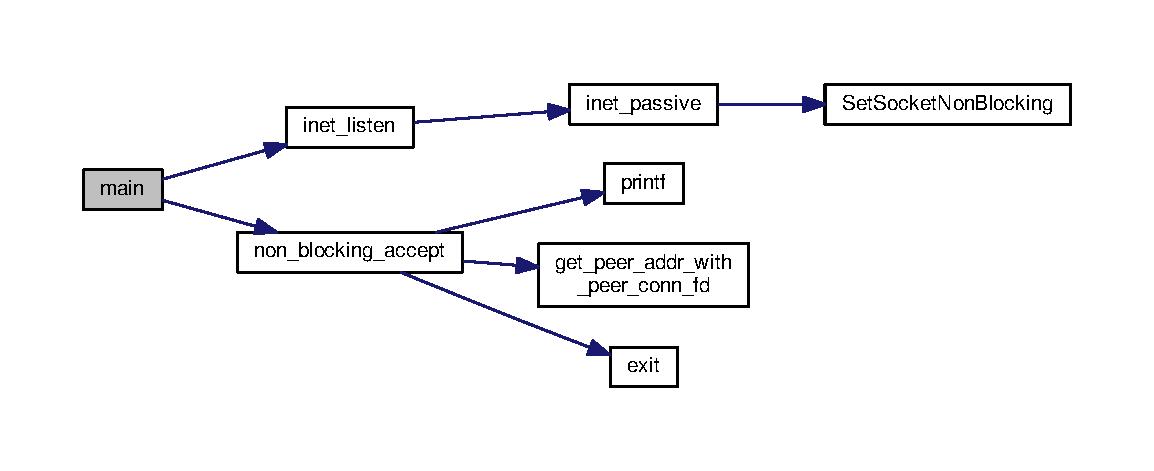
\includegraphics[width=350pt]{df/dd7/server_8cpp_a0ddf1224851353fc92bfbff6f499fa97_cgraph}
\end{center}
\end{figure}



\hypertarget{error__functions_8h}{\section{common/include/error\-\_\-functions.h File Reference}
\label{error__functions_8h}\index{common/include/error\-\_\-functions.\-h@{common/include/error\-\_\-functions.\-h}}
}
This graph shows which files directly or indirectly include this file\-:
\nopagebreak
\begin{figure}[H]
\begin{center}
\leavevmode
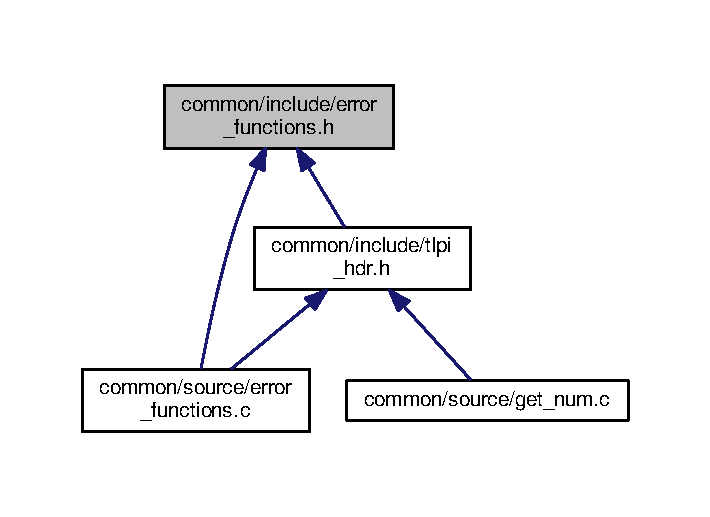
\includegraphics[width=341pt]{d2/d14/error__functions_8h__dep__incl}
\end{center}
\end{figure}
\subsection*{Macros}
\begin{DoxyCompactItemize}
\item 
\#define \hyperlink{error__functions_8h_aa1728270d73c5d1598de1fd691762eb1}{N\-O\-R\-E\-T\-U\-R\-N}
\end{DoxyCompactItemize}
\subsection*{Functions}
\begin{DoxyCompactItemize}
\item 
void \hyperlink{error__functions_8h_a46c1ae408432a2c70da4402236454a5f}{err\-Msg} (const char $\ast$format,...)
\begin{DoxyCompactList}\small\item\em \-: Method to print the message with errno message, without exit or \-\_\-exit call. \end{DoxyCompactList}\item 
void \hyperlink{error__functions_8h_aeb5543ed0c5dbefe48cc02bfe5ea4b9d}{err\-Exit} (const char $\ast$format,...) \hyperlink{error__functions_8h_aa1728270d73c5d1598de1fd691762eb1}{N\-O\-R\-E\-T\-U\-R\-N}
\begin{DoxyCompactList}\small\item\em \-: Method to print the message with errno message, with exit. \end{DoxyCompactList}\item 
void \hyperlink{error__functions_8h_a07d4874cc874a23a4a7250cb530ed181}{err\-\_\-exit} (const char $\ast$format,...) \hyperlink{error__functions_8h_aa1728270d73c5d1598de1fd691762eb1}{N\-O\-R\-E\-T\-U\-R\-N}
\begin{DoxyCompactList}\small\item\em \-: Method to print the message with errno message, with \-\_\-exit. \end{DoxyCompactList}\item 
void \hyperlink{error__functions_8h_a576bb071909f75db9021106ca17060ac}{err\-Exit\-E\-N} (int errnum, const char $\ast$format,...) \hyperlink{error__functions_8h_aa1728270d73c5d1598de1fd691762eb1}{N\-O\-R\-E\-T\-U\-R\-N}
\begin{DoxyCompactList}\small\item\em \-: Method to print the message with errno message, with exit call. \end{DoxyCompactList}\item 
void \hyperlink{error__functions_8h_a65272d8240c216ffa979ba66ba8eba87}{fatal} (const char $\ast$format,...) \hyperlink{error__functions_8h_aa1728270d73c5d1598de1fd691762eb1}{N\-O\-R\-E\-T\-U\-R\-N}
\begin{DoxyCompactList}\small\item\em \-: Method to print the message with errno message, with \-\_\-exit call. \end{DoxyCompactList}\item 
void \hyperlink{error__functions_8h_a332d03a26da0bbf12a47952696e0f5cf}{usage\-Err} (const char $\ast$format,...) \hyperlink{error__functions_8h_aa1728270d73c5d1598de1fd691762eb1}{N\-O\-R\-E\-T\-U\-R\-N}
\begin{DoxyCompactList}\small\item\em \-: Method to print the uses error. \end{DoxyCompactList}\item 
void \hyperlink{error__functions_8h_ab18ff8f52fc83c982f6b57454e82b44e}{cmd\-Line\-Err} (const char $\ast$format,...) \hyperlink{error__functions_8h_aa1728270d73c5d1598de1fd691762eb1}{N\-O\-R\-E\-T\-U\-R\-N}
\begin{DoxyCompactList}\small\item\em \-: Method to print the command line argument error. \end{DoxyCompactList}\end{DoxyCompactItemize}


\subsection{Macro Definition Documentation}
\hypertarget{error__functions_8h_aa1728270d73c5d1598de1fd691762eb1}{\index{error\-\_\-functions.\-h@{error\-\_\-functions.\-h}!N\-O\-R\-E\-T\-U\-R\-N@{N\-O\-R\-E\-T\-U\-R\-N}}
\index{N\-O\-R\-E\-T\-U\-R\-N@{N\-O\-R\-E\-T\-U\-R\-N}!error_functions.h@{error\-\_\-functions.\-h}}
\subsubsection[{N\-O\-R\-E\-T\-U\-R\-N}]{\setlength{\rightskip}{0pt plus 5cm}\#define N\-O\-R\-E\-T\-U\-R\-N}}\label{error__functions_8h_aa1728270d73c5d1598de1fd691762eb1}


Definition at line 9 of file error\-\_\-functions.\-h.



\subsection{Function Documentation}
\hypertarget{error__functions_8h_ab18ff8f52fc83c982f6b57454e82b44e}{\index{error\-\_\-functions.\-h@{error\-\_\-functions.\-h}!cmd\-Line\-Err@{cmd\-Line\-Err}}
\index{cmd\-Line\-Err@{cmd\-Line\-Err}!error_functions.h@{error\-\_\-functions.\-h}}
\subsubsection[{cmd\-Line\-Err}]{\setlength{\rightskip}{0pt plus 5cm}void cmd\-Line\-Err (
\begin{DoxyParamCaption}
\item[{const char $\ast$}]{format, }
\item[{}]{...}
\end{DoxyParamCaption}
)}}\label{error__functions_8h_ab18ff8f52fc83c982f6b57454e82b44e}


\-: Method to print the command line argument error. 

\begin{DoxyAuthor}{Author}
\-: Ravi Prasad (India) 
\end{DoxyAuthor}


Definition at line 188 of file error\-\_\-functions.\-c.

\hypertarget{error__functions_8h_a07d4874cc874a23a4a7250cb530ed181}{\index{error\-\_\-functions.\-h@{error\-\_\-functions.\-h}!err\-\_\-exit@{err\-\_\-exit}}
\index{err\-\_\-exit@{err\-\_\-exit}!error_functions.h@{error\-\_\-functions.\-h}}
\subsubsection[{err\-\_\-exit}]{\setlength{\rightskip}{0pt plus 5cm}void err\-\_\-exit (
\begin{DoxyParamCaption}
\item[{const char $\ast$}]{format, }
\item[{}]{...}
\end{DoxyParamCaption}
)}}\label{error__functions_8h_a07d4874cc874a23a4a7250cb530ed181}


\-: Method to print the message with errno message, with \-\_\-exit. 

\begin{DoxyAuthor}{Author}
\-: Ravi Prasad (India) 
\end{DoxyAuthor}


Definition at line 122 of file error\-\_\-functions.\-c.

\hypertarget{error__functions_8h_aeb5543ed0c5dbefe48cc02bfe5ea4b9d}{\index{error\-\_\-functions.\-h@{error\-\_\-functions.\-h}!err\-Exit@{err\-Exit}}
\index{err\-Exit@{err\-Exit}!error_functions.h@{error\-\_\-functions.\-h}}
\subsubsection[{err\-Exit}]{\setlength{\rightskip}{0pt plus 5cm}void err\-Exit (
\begin{DoxyParamCaption}
\item[{const char $\ast$}]{format, }
\item[{}]{...}
\end{DoxyParamCaption}
)}}\label{error__functions_8h_aeb5543ed0c5dbefe48cc02bfe5ea4b9d}


\-: Method to print the message with errno message, with exit. 

\begin{DoxyAuthor}{Author}
\-: Ravi Prasad (India) 
\end{DoxyAuthor}


Definition at line 106 of file error\-\_\-functions.\-c.

\hypertarget{error__functions_8h_a576bb071909f75db9021106ca17060ac}{\index{error\-\_\-functions.\-h@{error\-\_\-functions.\-h}!err\-Exit\-E\-N@{err\-Exit\-E\-N}}
\index{err\-Exit\-E\-N@{err\-Exit\-E\-N}!error_functions.h@{error\-\_\-functions.\-h}}
\subsubsection[{err\-Exit\-E\-N}]{\setlength{\rightskip}{0pt plus 5cm}void err\-Exit\-E\-N (
\begin{DoxyParamCaption}
\item[{int}]{err\-Num, }
\item[{const char $\ast$}]{format, }
\item[{}]{...}
\end{DoxyParamCaption}
)}}\label{error__functions_8h_a576bb071909f75db9021106ca17060ac}


\-: Method to print the message with errno message, with exit call. 

\begin{DoxyAuthor}{Author}
\-: Ravi Prasad (India) 
\end{DoxyAuthor}


Definition at line 138 of file error\-\_\-functions.\-c.

\hypertarget{error__functions_8h_a46c1ae408432a2c70da4402236454a5f}{\index{error\-\_\-functions.\-h@{error\-\_\-functions.\-h}!err\-Msg@{err\-Msg}}
\index{err\-Msg@{err\-Msg}!error_functions.h@{error\-\_\-functions.\-h}}
\subsubsection[{err\-Msg}]{\setlength{\rightskip}{0pt plus 5cm}void err\-Msg (
\begin{DoxyParamCaption}
\item[{const char $\ast$}]{format, }
\item[{}]{...}
\end{DoxyParamCaption}
)}}\label{error__functions_8h_a46c1ae408432a2c70da4402236454a5f}


\-: Method to print the message with errno message, without exit or \-\_\-exit call. 

\begin{DoxyAuthor}{Author}
\-: Ravi Prasad (India) 
\end{DoxyAuthor}


Definition at line 88 of file error\-\_\-functions.\-c.



Here is the call graph for this function\-:
\nopagebreak
\begin{figure}[H]
\begin{center}
\leavevmode
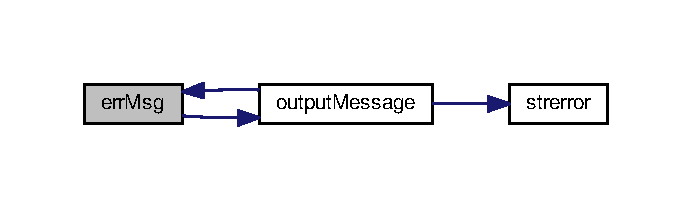
\includegraphics[width=332pt]{df/d33/error__functions_8h_a46c1ae408432a2c70da4402236454a5f_cgraph}
\end{center}
\end{figure}




Here is the caller graph for this function\-:
\nopagebreak
\begin{figure}[H]
\begin{center}
\leavevmode
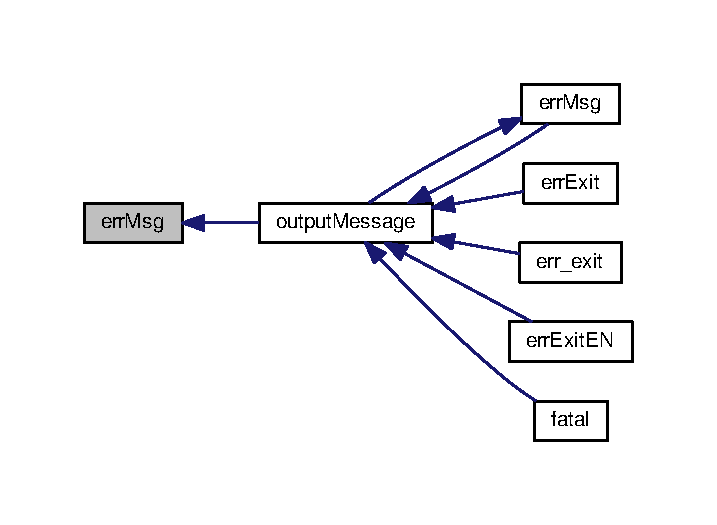
\includegraphics[width=344pt]{df/d33/error__functions_8h_a46c1ae408432a2c70da4402236454a5f_icgraph}
\end{center}
\end{figure}


\hypertarget{error__functions_8h_a65272d8240c216ffa979ba66ba8eba87}{\index{error\-\_\-functions.\-h@{error\-\_\-functions.\-h}!fatal@{fatal}}
\index{fatal@{fatal}!error_functions.h@{error\-\_\-functions.\-h}}
\subsubsection[{fatal}]{\setlength{\rightskip}{0pt plus 5cm}void fatal (
\begin{DoxyParamCaption}
\item[{const char $\ast$}]{format, }
\item[{}]{...}
\end{DoxyParamCaption}
)}}\label{error__functions_8h_a65272d8240c216ffa979ba66ba8eba87}


\-: Method to print the message with errno message, with \-\_\-exit call. 

\begin{DoxyAuthor}{Author}
\-: Ravi Prasad (India) 
\end{DoxyAuthor}


Definition at line 154 of file error\-\_\-functions.\-c.



Here is the call graph for this function\-:
\nopagebreak
\begin{figure}[H]
\begin{center}
\leavevmode
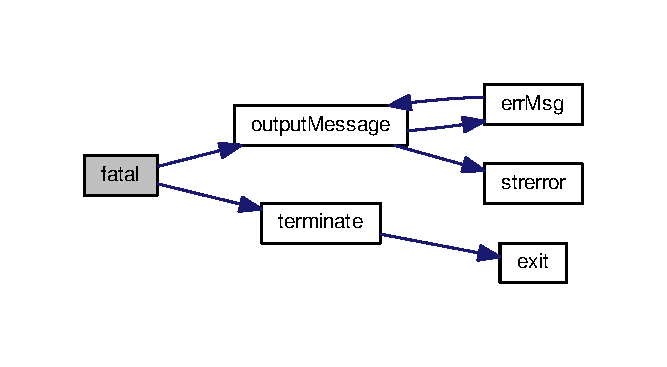
\includegraphics[width=320pt]{df/d33/error__functions_8h_a65272d8240c216ffa979ba66ba8eba87_cgraph}
\end{center}
\end{figure}


\hypertarget{error__functions_8h_a332d03a26da0bbf12a47952696e0f5cf}{\index{error\-\_\-functions.\-h@{error\-\_\-functions.\-h}!usage\-Err@{usage\-Err}}
\index{usage\-Err@{usage\-Err}!error_functions.h@{error\-\_\-functions.\-h}}
\subsubsection[{usage\-Err}]{\setlength{\rightskip}{0pt plus 5cm}void usage\-Err (
\begin{DoxyParamCaption}
\item[{const char $\ast$}]{format, }
\item[{}]{...}
\end{DoxyParamCaption}
)}}\label{error__functions_8h_a332d03a26da0bbf12a47952696e0f5cf}


\-: Method to print the uses error. 

\begin{DoxyAuthor}{Author}
\-: Ravi Prasad (India) 
\end{DoxyAuthor}


Definition at line 169 of file error\-\_\-functions.\-c.


\hypertarget{get__num_8h}{\section{common/include/get\-\_\-num.h File Reference}
\label{get__num_8h}\index{common/include/get\-\_\-num.\-h@{common/include/get\-\_\-num.\-h}}
}
{\ttfamily \#include $<$stdio.\-h$>$}\\*
{\ttfamily \#include $<$limits.\-h$>$}\\*
Include dependency graph for get\-\_\-num.\-h\-:
\nopagebreak
\begin{figure}[H]
\begin{center}
\leavevmode
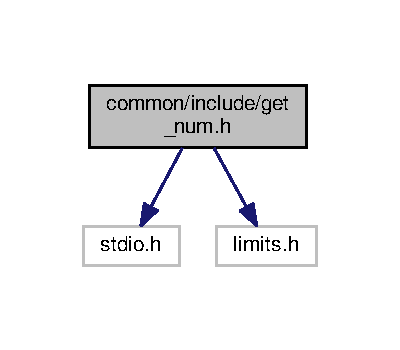
\includegraphics[width=192pt]{d3/d07/get__num_8h__incl}
\end{center}
\end{figure}
This graph shows which files directly or indirectly include this file\-:
\nopagebreak
\begin{figure}[H]
\begin{center}
\leavevmode
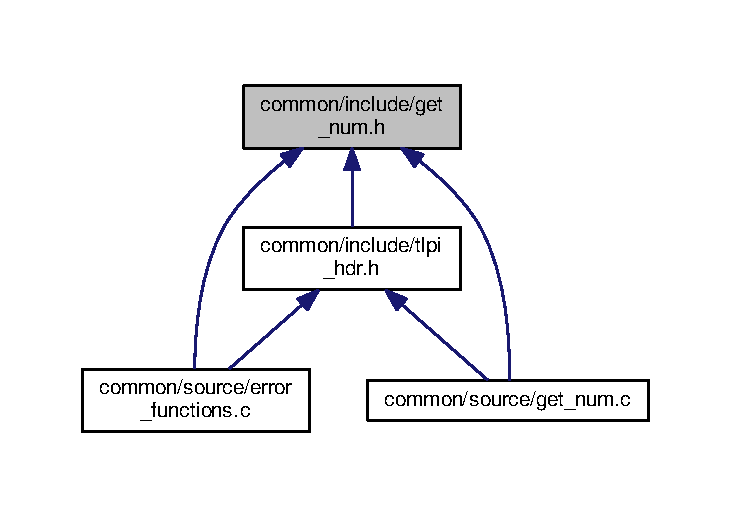
\includegraphics[width=350pt]{d7/d78/get__num_8h__dep__incl}
\end{center}
\end{figure}
\subsection*{Functions}
\begin{DoxyCompactItemize}
\item 
int \hyperlink{get__num_8h_aafea1112c7333dcfa49a8d051c2bde9a}{my\-Atoi} (char $\ast$str)
\item 
long \hyperlink{get__num_8h_afc17dbeb125e1388078e1a9221624f15}{my\-Atol} (char $\ast$str)
\end{DoxyCompactItemize}


\subsection{Function Documentation}
\hypertarget{get__num_8h_aafea1112c7333dcfa49a8d051c2bde9a}{\index{get\-\_\-num.\-h@{get\-\_\-num.\-h}!my\-Atoi@{my\-Atoi}}
\index{my\-Atoi@{my\-Atoi}!get_num.h@{get\-\_\-num.\-h}}
\subsubsection[{my\-Atoi}]{\setlength{\rightskip}{0pt plus 5cm}int my\-Atoi (
\begin{DoxyParamCaption}
\item[{char $\ast$}]{str}
\end{DoxyParamCaption}
)}}\label{get__num_8h_aafea1112c7333dcfa49a8d051c2bde9a}
cutomize atoi 

Definition at line 12 of file get\-\_\-num.\-c.



Here is the call graph for this function\-:
\nopagebreak
\begin{figure}[H]
\begin{center}
\leavevmode
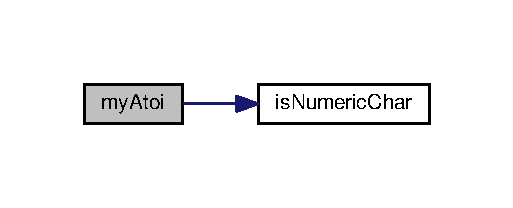
\includegraphics[width=246pt]{d6/d3b/get__num_8h_aafea1112c7333dcfa49a8d051c2bde9a_cgraph}
\end{center}
\end{figure}


\hypertarget{get__num_8h_afc17dbeb125e1388078e1a9221624f15}{\index{get\-\_\-num.\-h@{get\-\_\-num.\-h}!my\-Atol@{my\-Atol}}
\index{my\-Atol@{my\-Atol}!get_num.h@{get\-\_\-num.\-h}}
\subsubsection[{my\-Atol}]{\setlength{\rightskip}{0pt plus 5cm}long my\-Atol (
\begin{DoxyParamCaption}
\item[{char $\ast$}]{str}
\end{DoxyParamCaption}
)}}\label{get__num_8h_afc17dbeb125e1388078e1a9221624f15}


Definition at line 44 of file get\-\_\-num.\-c.



Here is the call graph for this function\-:
\nopagebreak
\begin{figure}[H]
\begin{center}
\leavevmode
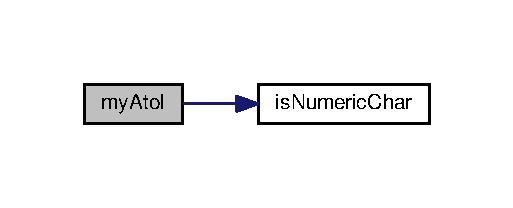
\includegraphics[width=246pt]{d6/d3b/get__num_8h_afc17dbeb125e1388078e1a9221624f15_cgraph}
\end{center}
\end{figure}



\hypertarget{tlpi__hdr_8h}{\section{common/include/tlpi\-\_\-hdr.h File Reference}
\label{tlpi__hdr_8h}\index{common/include/tlpi\-\_\-hdr.\-h@{common/include/tlpi\-\_\-hdr.\-h}}
}
{\ttfamily \#include $<$sys/types.\-h$>$}\\*
{\ttfamily \#include $<$stdio.\-h$>$}\\*
{\ttfamily \#include $<$stdlib.\-h$>$}\\*
{\ttfamily \#include $<$unistd.\-h$>$}\\*
{\ttfamily \#include $<$errno.\-h$>$}\\*
{\ttfamily \#include $<$string.\-h$>$}\\*
{\ttfamily \#include \char`\"{}get\-\_\-num.\-h\char`\"{}}\\*
{\ttfamily \#include \char`\"{}error\-\_\-functions.\-h\char`\"{}}\\*
Include dependency graph for tlpi\-\_\-hdr.\-h\-:
\nopagebreak
\begin{figure}[H]
\begin{center}
\leavevmode
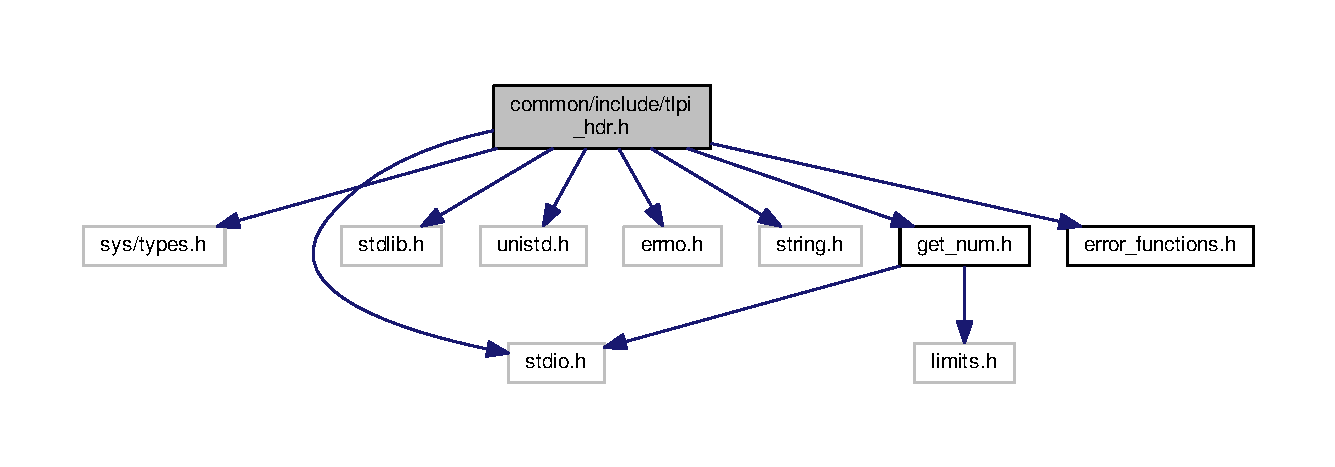
\includegraphics[width=350pt]{de/de5/tlpi__hdr_8h__incl}
\end{center}
\end{figure}
This graph shows which files directly or indirectly include this file\-:
\nopagebreak
\begin{figure}[H]
\begin{center}
\leavevmode
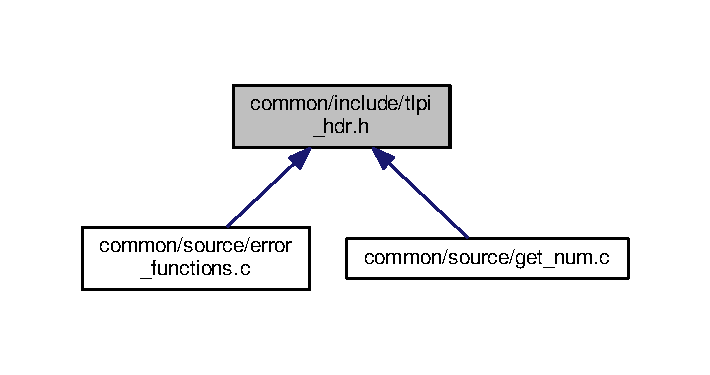
\includegraphics[width=341pt]{df/df0/tlpi__hdr_8h__dep__incl}
\end{center}
\end{figure}
\subsection*{Macros}
\begin{DoxyCompactItemize}
\item 
\#define \hyperlink{tlpi__hdr_8h_a2a9e49dec41ddabf74cd01742996228f}{T\-L\-P\-I\-\_\-\-H\-D\-R\-\_\-\-H}~/$\ast$ Prevent accidental double inclusion $\ast$/
\item 
\#define \hyperlink{tlpi__hdr_8h_a69db94a857e4ed0645c48085b2e3bd0a}{min}(m, n)~((m) $<$ (n) ? (m) \-: (n))
\item 
\#define \hyperlink{tlpi__hdr_8h_aae5d226fe30fc72743bf5b8b3d691fe7}{max}(m, n)~((m) $>$ (n) ? (m) \-: (n))
\end{DoxyCompactItemize}
\subsection*{Enumerations}
\begin{DoxyCompactItemize}
\item 
enum \hyperlink{tlpi__hdr_8h_aec7e62084419d7857ae740a4c68241cf}{B\-O\-O\-L\-E\-A\-N} \{ \hyperlink{tlpi__hdr_8h_aec7e62084419d7857ae740a4c68241cfaa1e095cc966dbecf6a0d8aad75348d1a}{F\-A\-L\-S\-E}, 
\hyperlink{tlpi__hdr_8h_aec7e62084419d7857ae740a4c68241cfaa82764c3079aea4e60c80e45befbb839}{T\-R\-U\-E}
 \}
\end{DoxyCompactItemize}


\subsection{Macro Definition Documentation}
\hypertarget{tlpi__hdr_8h_aae5d226fe30fc72743bf5b8b3d691fe7}{\index{tlpi\-\_\-hdr.\-h@{tlpi\-\_\-hdr.\-h}!max@{max}}
\index{max@{max}!tlpi_hdr.h@{tlpi\-\_\-hdr.\-h}}
\subsubsection[{max}]{\setlength{\rightskip}{0pt plus 5cm}\#define max(
\begin{DoxyParamCaption}
\item[{}]{m, }
\item[{}]{n}
\end{DoxyParamCaption}
)~((m) $>$ (n) ? (m) \-: (n))}}\label{tlpi__hdr_8h_aae5d226fe30fc72743bf5b8b3d691fe7}


Definition at line 16 of file tlpi\-\_\-hdr.\-h.

\hypertarget{tlpi__hdr_8h_a69db94a857e4ed0645c48085b2e3bd0a}{\index{tlpi\-\_\-hdr.\-h@{tlpi\-\_\-hdr.\-h}!min@{min}}
\index{min@{min}!tlpi_hdr.h@{tlpi\-\_\-hdr.\-h}}
\subsubsection[{min}]{\setlength{\rightskip}{0pt plus 5cm}\#define min(
\begin{DoxyParamCaption}
\item[{}]{m, }
\item[{}]{n}
\end{DoxyParamCaption}
)~((m) $<$ (n) ? (m) \-: (n))}}\label{tlpi__hdr_8h_a69db94a857e4ed0645c48085b2e3bd0a}


Definition at line 15 of file tlpi\-\_\-hdr.\-h.

\hypertarget{tlpi__hdr_8h_a2a9e49dec41ddabf74cd01742996228f}{\index{tlpi\-\_\-hdr.\-h@{tlpi\-\_\-hdr.\-h}!T\-L\-P\-I\-\_\-\-H\-D\-R\-\_\-\-H@{T\-L\-P\-I\-\_\-\-H\-D\-R\-\_\-\-H}}
\index{T\-L\-P\-I\-\_\-\-H\-D\-R\-\_\-\-H@{T\-L\-P\-I\-\_\-\-H\-D\-R\-\_\-\-H}!tlpi_hdr.h@{tlpi\-\_\-hdr.\-h}}
\subsubsection[{T\-L\-P\-I\-\_\-\-H\-D\-R\-\_\-\-H}]{\setlength{\rightskip}{0pt plus 5cm}\#define T\-L\-P\-I\-\_\-\-H\-D\-R\-\_\-\-H~/$\ast$ Prevent accidental double inclusion $\ast$/}}\label{tlpi__hdr_8h_a2a9e49dec41ddabf74cd01742996228f}


Definition at line 2 of file tlpi\-\_\-hdr.\-h.



\subsection{Enumeration Type Documentation}
\hypertarget{tlpi__hdr_8h_aec7e62084419d7857ae740a4c68241cf}{\index{tlpi\-\_\-hdr.\-h@{tlpi\-\_\-hdr.\-h}!B\-O\-O\-L\-E\-A\-N@{B\-O\-O\-L\-E\-A\-N}}
\index{B\-O\-O\-L\-E\-A\-N@{B\-O\-O\-L\-E\-A\-N}!tlpi_hdr.h@{tlpi\-\_\-hdr.\-h}}
\subsubsection[{B\-O\-O\-L\-E\-A\-N}]{\setlength{\rightskip}{0pt plus 5cm}enum {\bf B\-O\-O\-L\-E\-A\-N}}}\label{tlpi__hdr_8h_aec7e62084419d7857ae740a4c68241cf}
\begin{Desc}
\item[Enumerator]\par
\begin{description}
\index{F\-A\-L\-S\-E@{F\-A\-L\-S\-E}!tlpi\-\_\-hdr.\-h@{tlpi\-\_\-hdr.\-h}}\index{tlpi\-\_\-hdr.\-h@{tlpi\-\_\-hdr.\-h}!F\-A\-L\-S\-E@{F\-A\-L\-S\-E}}\item[{\em 
\hypertarget{tlpi__hdr_8h_aec7e62084419d7857ae740a4c68241cfaa1e095cc966dbecf6a0d8aad75348d1a}{F\-A\-L\-S\-E}\label{tlpi__hdr_8h_aec7e62084419d7857ae740a4c68241cfaa1e095cc966dbecf6a0d8aad75348d1a}
}]\index{T\-R\-U\-E@{T\-R\-U\-E}!tlpi\-\_\-hdr.\-h@{tlpi\-\_\-hdr.\-h}}\index{tlpi\-\_\-hdr.\-h@{tlpi\-\_\-hdr.\-h}!T\-R\-U\-E@{T\-R\-U\-E}}\item[{\em 
\hypertarget{tlpi__hdr_8h_aec7e62084419d7857ae740a4c68241cfaa82764c3079aea4e60c80e45befbb839}{T\-R\-U\-E}\label{tlpi__hdr_8h_aec7e62084419d7857ae740a4c68241cfaa82764c3079aea4e60c80e45befbb839}
}]\end{description}
\end{Desc}


Definition at line 14 of file tlpi\-\_\-hdr.\-h.


\hypertarget{common_2README}{\section{common/\-R\-E\-A\-D\-M\-E File Reference}
\label{common_2README}\index{common/\-R\-E\-A\-D\-M\-E@{common/\-R\-E\-A\-D\-M\-E}}
}
\subsection*{Functions}
\begin{DoxyCompactItemize}
\item 
$\ast$$\ast$$\ast$$\ast$$\ast$$\ast$$\ast$$\ast$$\ast$$\ast$$\ast$$\ast$$\ast$$\ast$$\ast$$\ast$$\ast$$\ast$$\ast$$\ast$$\ast$$\ast$$\ast$$\ast$$\ast$$\ast$$\ast$$\ast$Calls \\*
which sets \hyperlink{common_2README_afe75ee0c7e5a90ba6bb38426ea69b996}{errno} \\*
$\ast$$\ast$$\ast$$\ast$$\ast$$\ast$$\ast$$\ast$$\ast$$\ast$$\ast$$\ast$$\ast$$\ast$$\ast$$\ast$$\ast$$\ast$$\ast$$\ast$$\ast$$\ast$$\ast$$\ast$$\ast$$\ast$$\ast$$\ast$To \\*
diagnose \hyperlink{common_2README_a9912daeb8cc621a6ee8e1d24ebdbe601}{errors} from system \\*
calls and \hyperlink{ClientServer_2server_2Makefile_a1f477410360bd4832116581b9934ab71}{library} we use \hyperlink{common_2README_a83413e40798cc613af12fa88a21035a5}{err\-Msg} ()
\item 
$\ast$$\ast$$\ast$$\ast$$\ast$$\ast$$\ast$$\ast$$\ast$$\ast$$\ast$$\ast$$\ast$$\ast$$\ast$$\ast$$\ast$$\ast$$\ast$$\ast$$\ast$$\ast$$\ast$$\ast$$\ast$$\ast$$\ast$$\ast$Calls \\*
which sets \hyperlink{common_2README_afe75ee0c7e5a90ba6bb38426ea69b996}{errno} \\*
$\ast$$\ast$$\ast$$\ast$$\ast$$\ast$$\ast$$\ast$$\ast$$\ast$$\ast$$\ast$$\ast$$\ast$$\ast$$\ast$$\ast$$\ast$$\ast$$\ast$$\ast$$\ast$$\ast$$\ast$$\ast$$\ast$$\ast$$\ast$To \\*
diagnose \hyperlink{common_2README_a9912daeb8cc621a6ee8e1d24ebdbe601}{errors} from system \\*
calls and \hyperlink{ClientServer_2server_2Makefile_a1f477410360bd4832116581b9934ab71}{library} we use \hyperlink{common_2README_a68943fd8366445b15b2c72863bbc5b01}{err\-Exit} ()
\item 
$\ast$$\ast$$\ast$$\ast$$\ast$$\ast$$\ast$$\ast$$\ast$$\ast$$\ast$$\ast$$\ast$$\ast$$\ast$$\ast$$\ast$$\ast$$\ast$$\ast$$\ast$$\ast$$\ast$$\ast$$\ast$$\ast$$\ast$$\ast$Calls \\*
which sets \hyperlink{common_2README_afe75ee0c7e5a90ba6bb38426ea69b996}{errno} \\*
$\ast$$\ast$$\ast$$\ast$$\ast$$\ast$$\ast$$\ast$$\ast$$\ast$$\ast$$\ast$$\ast$$\ast$$\ast$$\ast$$\ast$$\ast$$\ast$$\ast$$\ast$$\ast$$\ast$$\ast$$\ast$$\ast$$\ast$$\ast$To \\*
diagnose \hyperlink{common_2README_a9912daeb8cc621a6ee8e1d24ebdbe601}{errors} from system \\*
calls and \hyperlink{ClientServer_2server_2Makefile_a1f477410360bd4832116581b9934ab71}{library} we use \hyperlink{common_2README_ad0cc7e68335dc54caa4465fe0ca45c21}{err\-\_\-exit} ()
\item 
$\ast$$\ast$$\ast$$\ast$$\ast$$\ast$$\ast$$\ast$$\ast$$\ast$$\ast$$\ast$$\ast$$\ast$$\ast$$\ast$$\ast$$\ast$$\ast$$\ast$$\ast$$\ast$$\ast$$\ast$$\ast$$\ast$$\ast$$\ast$Calls \\*
which sets \hyperlink{common_2README_afe75ee0c7e5a90ba6bb38426ea69b996}{errno} \\*
$\ast$$\ast$$\ast$$\ast$$\ast$$\ast$$\ast$$\ast$$\ast$$\ast$$\ast$$\ast$$\ast$$\ast$$\ast$$\ast$$\ast$$\ast$$\ast$$\ast$$\ast$$\ast$$\ast$$\ast$$\ast$$\ast$$\ast$$\ast$To \\*
diagnose \hyperlink{common_2README_a9912daeb8cc621a6ee8e1d24ebdbe601}{errors} from system \\*
calls and \hyperlink{ClientServer_2server_2Makefile_a1f477410360bd4832116581b9934ab71}{library} we use and \hyperlink{common_2README_a7c791eab42a732b614ef10956cc9b101}{err\-Exit\-E\-N} ().
\item 
void \hyperlink{common_2README_a9353730adacb3417493e841dace8708b}{err\-Exit} (const char $\ast$format,...)
\begin{DoxyCompactList}\small\item\em \-: Method to print the message with errno message, with exit. \end{DoxyCompactList}\item 
void \hyperlink{common_2README_ad83bc66851be4582ec97ba670a95fa0a}{err\-\_\-exit} (const char $\ast$format,...)
\begin{DoxyCompactList}\small\item\em \-: Method to print the message with errno message, with \-\_\-exit. \end{DoxyCompactList}\item 
void \hyperlink{common_2README_a6d6d5790ca5bffa970baeeefd8a28462}{err\-Exit\-E\-N} (int errnum, const char $\ast$format,...)
\begin{DoxyCompactList}\small\item\em \-: Method to print the message with errno message, with exit call. \end{DoxyCompactList}\item 
except that a terminating \\*
newline character is \\*
automatically appended to \hyperlink{ClientServer_2server_2Makefile_a09c6b60bb7451f9136e25140ffdff6bd}{the} \\*
output string The such as plus \\*
\hyperlink{ClientServer_2server_2Makefile_a09c6b60bb7451f9136e25140ffdff6bd}{the} \hyperlink{common_2README_a80171b13188418b4328f9247d3aff3d2}{error} description as \\*
returned by \hyperlink{common_2README_af3164892dd3bd1beaa3a2b70e01edcd9}{strerror} () —followed by \hyperlink{ClientServer_2server_2Makefile_a09c6b60bb7451f9136e25140ffdff6bd}{the} formatted output specified in \hyperlink{ClientServer_2server_2Makefile_a09c6b60bb7451f9136e25140ffdff6bd}{the} argument list.\-The \hyperlink{error__functions_8c_a9353730adacb3417493e841dace8708b}{err\-Exit}() function operates like \hyperlink{error__functions_8c_a46c1ae408432a2c70da4402236454a5f}{err\-Msg}()
\item 
except that a terminating \\*
newline character is \\*
automatically appended to \hyperlink{ClientServer_2server_2Makefile_a09c6b60bb7451f9136e25140ffdff6bd}{the} \\*
output string The such as plus \\*
\hyperlink{ClientServer_2server_2Makefile_a09c6b60bb7451f9136e25140ffdff6bd}{the} \hyperlink{common_2README_a80171b13188418b4328f9247d3aff3d2}{error} description as \\*
returned by but also \\*
terminates \hyperlink{ClientServer_2server_2Makefile_a09c6b60bb7451f9136e25140ffdff6bd}{the} by calling \hyperlink{common_2README_a85c39bfe84eed5e1d7dae87fb0018669}{exit} ().The \hyperlink{error__functions_8c_ad83bc66851be4582ec97ba670a95fa0a}{err\-\_\-exit}() function is similar to \hyperlink{error__functions_8c_a9353730adacb3417493e841dace8708b}{err\-Exit}()
\item 
except that a terminating \\*
newline character is \\*
automatically appended to \hyperlink{ClientServer_2server_2Makefile_a09c6b60bb7451f9136e25140ffdff6bd}{the} \\*
output string The such as plus \\*
\hyperlink{ClientServer_2server_2Makefile_a09c6b60bb7451f9136e25140ffdff6bd}{the} \hyperlink{common_2README_a80171b13188418b4328f9247d3aff3d2}{error} description as \\*
returned by but also \\*
terminates \hyperlink{ClientServer_2server_2Makefile_a09c6b60bb7451f9136e25140ffdff6bd}{the} by calling but \\*
differs in two except that \\*
instead of printing \hyperlink{ClientServer_2server_2Makefile_a09c6b60bb7451f9136e25140ffdff6bd}{the} \hyperlink{common_2README_a80171b13188418b4328f9247d3aff3d2}{error} \\*
text corresponding to \hyperlink{ClientServer_2server_2Makefile_a09c6b60bb7451f9136e25140ffdff6bd}{the} \\*
current value of it prints \hyperlink{ClientServer_2server_2Makefile_a09c6b60bb7451f9136e25140ffdff6bd}{the} \\*
text corresponding to \hyperlink{ClientServer_2server_2Makefile_a09c6b60bb7451f9136e25140ffdff6bd}{the} \\*
\hyperlink{common_2README_a80171b13188418b4328f9247d3aff3d2}{error} \hyperlink{common_2README_aba79e3975c1b7da6e77c2f4b561603ae}{number} (thus, \hyperlink{ClientServer_2server_2Makefile_a09c6b60bb7451f9136e25140ffdff6bd}{the} E\-N suffix) given in \hyperlink{ClientServer_2server_2Makefile_a09c6b60bb7451f9136e25140ffdff6bd}{the} argument errnum.\-Mainly
\item 
except that a terminating \\*
newline character is \\*
automatically appended to \hyperlink{ClientServer_2server_2Makefile_a09c6b60bb7451f9136e25140ffdff6bd}{the} \\*
output string The such as plus \\*
\hyperlink{ClientServer_2server_2Makefile_a09c6b60bb7451f9136e25140ffdff6bd}{the} \hyperlink{common_2README_a80171b13188418b4328f9247d3aff3d2}{error} description as \\*
returned by but also \\*
terminates \hyperlink{ClientServer_2server_2Makefile_a09c6b60bb7451f9136e25140ffdff6bd}{the} by calling but \\*
differs in two except that \\*
instead of printing \hyperlink{ClientServer_2server_2Makefile_a09c6b60bb7451f9136e25140ffdff6bd}{the} \hyperlink{common_2README_a80171b13188418b4328f9247d3aff3d2}{error} \\*
text corresponding to \hyperlink{ClientServer_2server_2Makefile_a09c6b60bb7451f9136e25140ffdff6bd}{the} \\*
current value of it prints \hyperlink{ClientServer_2server_2Makefile_a09c6b60bb7451f9136e25140ffdff6bd}{the} \\*
text corresponding to \hyperlink{ClientServer_2server_2Makefile_a09c6b60bb7451f9136e25140ffdff6bd}{the} \\*
\hyperlink{common_2README_a80171b13188418b4328f9247d3aff3d2}{error} we use which return –1 \\*
on \hyperlink{ClientServer_2server_2Makefile_a09c6b60bb7451f9136e25140ffdff6bd}{the} P\-O\-S\-I\-X threads \hyperlink{common_2README_a853571ba73c010b99ff2788a0cfe4395}{functions} \\*
diagnose an \hyperlink{common_2README_a80171b13188418b4328f9247d3aff3d2}{error} by returning \\*
an \hyperlink{common_2README_a80171b13188418b4328f9247d3aff3d2}{error} \hyperlink{common_2README_aba79e3975c1b7da6e77c2f4b561603ae}{number}(i.\-e., a \\*
positive \hyperlink{common_2README_aba79e3975c1b7da6e77c2f4b561603ae}{number} of \hyperlink{ClientServer_2server_2Makefile_a09c6b60bb7451f9136e25140ffdff6bd}{the} type \\*
normally placed in \hyperlink{common_2README_afe75ee0c7e5a90ba6bb38426ea69b996}{errno}) as \\*
their function result.(The \\*
P\-O\-S\-I\-X threads \hyperlink{common_2README_a853571ba73c010b99ff2788a0cfe4395}{functions} return \\*
0 on success.) Example \hyperlink{common_2README_aaa5f75c9c764c204bf342e6b6cc969f6}{err\-Exit\-E\-N} (s,\char`\"{}pthread\-\_\-create\char`\"{})
\item 
$\ast$$\ast$$\ast$$\ast$$\ast$$\ast$$\ast$$\ast$$\ast$$\ast$$\ast$$\ast$$\ast$$\ast$$\ast$$\ast$$\ast$$\ast$$\ast$$\ast$$\ast$$\ast$$\ast$$\ast$$\ast$$\ast$$\ast$$\ast$$\ast$$\ast$$\ast$$\ast$$\ast$$\ast$$\ast$$\ast$$\ast$$\ast$$\ast$$\ast$$\ast$Calls \\*
which doesn t sets \hyperlink{common_2README_afe75ee0c7e5a90ba6bb38426ea69b996}{errno} \\*
$\ast$$\ast$$\ast$$\ast$$\ast$$\ast$$\ast$$\ast$$\ast$$\ast$$\ast$$\ast$$\ast$$\ast$$\ast$$\ast$$\ast$$\ast$$\ast$$\ast$$\ast$$\ast$$\ast$$\ast$$\ast$$\ast$$\ast$$\ast$$\ast$$\ast$$\ast$$\ast$$\ast$$\ast$$\ast$$\ast$$\ast$$\ast$$\ast$$\ast$$\ast$To \\*
diagnose other types of we use \hyperlink{common_2README_ae688a97aa2b3eb3a27322a140be60049}{fatal} ()
\item 
$\ast$$\ast$$\ast$$\ast$$\ast$$\ast$$\ast$$\ast$$\ast$$\ast$$\ast$$\ast$$\ast$$\ast$$\ast$$\ast$$\ast$$\ast$$\ast$$\ast$$\ast$$\ast$$\ast$$\ast$$\ast$$\ast$$\ast$$\ast$$\ast$$\ast$$\ast$$\ast$$\ast$$\ast$$\ast$$\ast$$\ast$$\ast$$\ast$$\ast$$\ast$Calls \\*
which doesn t sets \hyperlink{common_2README_afe75ee0c7e5a90ba6bb38426ea69b996}{errno} \\*
$\ast$$\ast$$\ast$$\ast$$\ast$$\ast$$\ast$$\ast$$\ast$$\ast$$\ast$$\ast$$\ast$$\ast$$\ast$$\ast$$\ast$$\ast$$\ast$$\ast$$\ast$$\ast$$\ast$$\ast$$\ast$$\ast$$\ast$$\ast$$\ast$$\ast$$\ast$$\ast$$\ast$$\ast$$\ast$$\ast$$\ast$$\ast$$\ast$$\ast$$\ast$To \\*
diagnose other types of we use \hyperlink{common_2README_aff916c132f7e6f0b0dec6d7c28ee2573}{usage\-Err} ()
\item 
$\ast$$\ast$$\ast$$\ast$$\ast$$\ast$$\ast$$\ast$$\ast$$\ast$$\ast$$\ast$$\ast$$\ast$$\ast$$\ast$$\ast$$\ast$$\ast$$\ast$$\ast$$\ast$$\ast$$\ast$$\ast$$\ast$$\ast$$\ast$$\ast$$\ast$$\ast$$\ast$$\ast$$\ast$$\ast$$\ast$$\ast$$\ast$$\ast$$\ast$$\ast$Calls \\*
which doesn t sets \hyperlink{common_2README_afe75ee0c7e5a90ba6bb38426ea69b996}{errno} \\*
$\ast$$\ast$$\ast$$\ast$$\ast$$\ast$$\ast$$\ast$$\ast$$\ast$$\ast$$\ast$$\ast$$\ast$$\ast$$\ast$$\ast$$\ast$$\ast$$\ast$$\ast$$\ast$$\ast$$\ast$$\ast$$\ast$$\ast$$\ast$$\ast$$\ast$$\ast$$\ast$$\ast$$\ast$$\ast$$\ast$$\ast$$\ast$$\ast$$\ast$$\ast$To \\*
diagnose other types of we use \\*
and \hyperlink{common_2README_a63ccbdd536fd5a8c256b6aba4bab691a}{cmd\-Line\-Err} ().
\item 
void \hyperlink{common_2README_a0c81140d074e6630634e05e7ca437390}{usage\-Err} (const char $\ast$format,...)
\begin{DoxyCompactList}\small\item\em \-: Method to print the uses error. \end{DoxyCompactList}\item 
void \hyperlink{common_2README_a2998a663efe6e91b3870e2bb7fba5504}{cmd\-Line\-Err} (const char $\ast$format,...)
\begin{DoxyCompactList}\small\item\em \-: Method to print the command line argument error. \end{DoxyCompactList}\item 
including \hyperlink{common_2README_a9912daeb8cc621a6ee8e1d24ebdbe601}{errors} from \hyperlink{ClientServer_2server_2Makefile_a1f477410360bd4832116581b9934ab71}{library} \\*
\hyperlink{common_2README_a853571ba73c010b99ff2788a0cfe4395}{functions} that don’t set \\*
\hyperlink{common_2README_afe75ee0c7e5a90ba6bb38426ea69b996}{errno} Its argument list is \hyperlink{ClientServer_2server_2Makefile_a09c6b60bb7451f9136e25140ffdff6bd}{the} \\*
same as for \hyperlink{common_2README_ae46f6c5c5729768631dc5ff84e16d52b}{printf} ()
\end{DoxyCompactItemize}
\subsection*{Variables}
\begin{DoxyCompactItemize}
\item 
$\ast$$\ast$$\ast$$\ast$$\ast$$\ast$$\ast$$\ast$$\ast$$\ast$$\ast$$\ast$$\ast$$\ast$$\ast$$\ast$$\ast$$\ast$$\ast$$\ast$$\ast$$\ast$$\ast$$\ast$$\ast$$\ast$$\ast$$\ast$Calls \\*
which sets \hyperlink{common_2README_afe75ee0c7e5a90ba6bb38426ea69b996}{errno} \\*
$\ast$$\ast$$\ast$$\ast$$\ast$$\ast$$\ast$$\ast$$\ast$$\ast$$\ast$$\ast$$\ast$$\ast$$\ast$$\ast$$\ast$$\ast$$\ast$$\ast$$\ast$$\ast$$\ast$$\ast$$\ast$$\ast$$\ast$$\ast$To \\*
diagnose \hyperlink{common_2README_a9912daeb8cc621a6ee8e1d24ebdbe601}{errors} from system \\*
calls and \hyperlink{ClientServer_2server_2Makefile_a1f477410360bd4832116581b9934ab71}{library} \hyperlink{common_2README_a853571ba73c010b99ff2788a0cfe4395}{functions}
\item 
except that a terminating \\*
newline character is \\*
automatically appended to \hyperlink{ClientServer_2server_2Makefile_a09c6b60bb7451f9136e25140ffdff6bd}{the} \\*
output string The such as \hyperlink{common_2README_a9f655c76c94b7fe5fa4714a077ef4d7e}{E\-P\-E\-R\-M}
\item 
except that a terminating \\*
newline character is \\*
automatically appended to \hyperlink{ClientServer_2server_2Makefile_a09c6b60bb7451f9136e25140ffdff6bd}{the} \\*
output string The such as plus \\*
\hyperlink{ClientServer_2server_2Makefile_a09c6b60bb7451f9136e25140ffdff6bd}{the} \hyperlink{common_2README_a80171b13188418b4328f9247d3aff3d2}{error} description as \\*
returned by but also \\*
terminates \hyperlink{ClientServer_2server_2Makefile_a09c6b60bb7451f9136e25140ffdff6bd}{the} \hyperlink{common_2README_a2648c031e7768d2922f9bceca11215d9}{program}
\item 
except that a terminating \\*
newline character is \\*
automatically appended to \hyperlink{ClientServer_2server_2Makefile_a09c6b60bb7451f9136e25140ffdff6bd}{the} \\*
output string The such as plus \\*
\hyperlink{ClientServer_2server_2Makefile_a09c6b60bb7451f9136e25140ffdff6bd}{the} \hyperlink{common_2README_a80171b13188418b4328f9247d3aff3d2}{error} description as \\*
returned by but also \\*
terminates \hyperlink{ClientServer_2server_2Makefile_a09c6b60bb7451f9136e25140ffdff6bd}{the} by calling but \\*
differs in two \hyperlink{common_2README_a33a4706d30ee60d6fc7d0c4b387dc3b9}{respects}
\item 
except that a terminating \\*
newline character is \\*
automatically appended to \hyperlink{ClientServer_2server_2Makefile_a09c6b60bb7451f9136e25140ffdff6bd}{the} \\*
output string The such as plus \\*
\hyperlink{ClientServer_2server_2Makefile_a09c6b60bb7451f9136e25140ffdff6bd}{the} \hyperlink{common_2README_a80171b13188418b4328f9247d3aff3d2}{error} description as \\*
returned by but also \\*
terminates \hyperlink{ClientServer_2server_2Makefile_a09c6b60bb7451f9136e25140ffdff6bd}{the} by calling but \\*
differs in two except that \\*
instead of printing \hyperlink{ClientServer_2server_2Makefile_a09c6b60bb7451f9136e25140ffdff6bd}{the} \hyperlink{common_2README_a80171b13188418b4328f9247d3aff3d2}{error} \\*
text corresponding to \hyperlink{ClientServer_2server_2Makefile_a09c6b60bb7451f9136e25140ffdff6bd}{the} \\*
current value of \hyperlink{common_2README_afe75ee0c7e5a90ba6bb38426ea69b996}{errno}
\item 
except that a terminating \\*
newline character is \\*
automatically appended to \hyperlink{ClientServer_2server_2Makefile_a09c6b60bb7451f9136e25140ffdff6bd}{the} \\*
output string The such as plus \\*
\hyperlink{ClientServer_2server_2Makefile_a09c6b60bb7451f9136e25140ffdff6bd}{the} error description as \\*
returned by but also \\*
terminates \hyperlink{ClientServer_2server_2Makefile_a09c6b60bb7451f9136e25140ffdff6bd}{the} by calling but \\*
differs in two except that \\*
instead of printing \hyperlink{ClientServer_2server_2Makefile_a09c6b60bb7451f9136e25140ffdff6bd}{the} error \\*
text corresponding to \hyperlink{ClientServer_2server_2Makefile_a09c6b60bb7451f9136e25140ffdff6bd}{the} \\*
current value of it prints \hyperlink{ClientServer_2server_2Makefile_a09c6b60bb7451f9136e25140ffdff6bd}{the} \\*
text corresponding to \hyperlink{ClientServer_2server_2Makefile_a09c6b60bb7451f9136e25140ffdff6bd}{the} \\*
error we use which return –1 \\*
on \hyperlink{common_2README_a80171b13188418b4328f9247d3aff3d2}{error}
\item 
$\ast$$\ast$$\ast$$\ast$$\ast$$\ast$$\ast$$\ast$$\ast$$\ast$$\ast$$\ast$$\ast$$\ast$$\ast$$\ast$$\ast$$\ast$$\ast$$\ast$$\ast$$\ast$$\ast$$\ast$$\ast$$\ast$$\ast$$\ast$$\ast$$\ast$$\ast$$\ast$$\ast$$\ast$$\ast$$\ast$$\ast$$\ast$$\ast$$\ast$$\ast$Calls \\*
which doesn t sets \hyperlink{common_2README_afe75ee0c7e5a90ba6bb38426ea69b996}{errno} \\*
$\ast$$\ast$$\ast$$\ast$$\ast$$\ast$$\ast$$\ast$$\ast$$\ast$$\ast$$\ast$$\ast$$\ast$$\ast$$\ast$$\ast$$\ast$$\ast$$\ast$$\ast$$\ast$$\ast$$\ast$$\ast$$\ast$$\ast$$\ast$$\ast$$\ast$$\ast$$\ast$$\ast$$\ast$$\ast$$\ast$$\ast$$\ast$$\ast$$\ast$$\ast$To \\*
diagnose other types of \hyperlink{common_2README_a9912daeb8cc621a6ee8e1d24ebdbe601}{errors}
\end{DoxyCompactItemize}


\subsection{Function Documentation}
\hypertarget{common_2README_a63ccbdd536fd5a8c256b6aba4bab691a}{\index{common/\-R\-E\-A\-D\-M\-E@{common/\-R\-E\-A\-D\-M\-E}!cmd\-Line\-Err@{cmd\-Line\-Err}}
\index{cmd\-Line\-Err@{cmd\-Line\-Err}!common/README@{common/\-R\-E\-A\-D\-M\-E}}
\subsubsection[{cmd\-Line\-Err}]{\setlength{\rightskip}{0pt plus 5cm}$\ast$$\ast$$\ast$$\ast$$\ast$$\ast$$\ast$$\ast$$\ast$$\ast$$\ast$$\ast$$\ast$$\ast$$\ast$$\ast$$\ast$$\ast$$\ast$$\ast$$\ast$$\ast$$\ast$$\ast$$\ast$$\ast$$\ast$$\ast$$\ast$$\ast$$\ast$$\ast$$\ast$$\ast$$\ast$$\ast$$\ast$$\ast$$\ast$$\ast$$\ast$ Calls which doesn t sets {\bf errno}$\ast$$\ast$$\ast$$\ast$$\ast$$\ast$$\ast$$\ast$$\ast$$\ast$$\ast$$\ast$$\ast$$\ast$$\ast$$\ast$$\ast$$\ast$$\ast$$\ast$$\ast$$\ast$$\ast$$\ast$$\ast$$\ast$$\ast$$\ast$$\ast$$\ast$$\ast$$\ast$$\ast$$\ast$$\ast$$\ast$$\ast$$\ast$$\ast$$\ast$$\ast$ To diagnose other types of we use and cmd\-Line\-Err (
\begin{DoxyParamCaption}
{}
\end{DoxyParamCaption}
)}}\label{common_2README_a63ccbdd536fd5a8c256b6aba4bab691a}
\hypertarget{common_2README_a2998a663efe6e91b3870e2bb7fba5504}{\index{common/\-R\-E\-A\-D\-M\-E@{common/\-R\-E\-A\-D\-M\-E}!cmd\-Line\-Err@{cmd\-Line\-Err}}
\index{cmd\-Line\-Err@{cmd\-Line\-Err}!common/README@{common/\-R\-E\-A\-D\-M\-E}}
\subsubsection[{cmd\-Line\-Err}]{\setlength{\rightskip}{0pt plus 5cm}void cmd\-Line\-Err (
\begin{DoxyParamCaption}
\item[{const char $\ast$}]{format, }
\item[{}]{...}
\end{DoxyParamCaption}
)}}\label{common_2README_a2998a663efe6e91b3870e2bb7fba5504}


\-: Method to print the command line argument error. 

\begin{DoxyAuthor}{Author}
\-: Ravi Prasad (India) 
\end{DoxyAuthor}


Definition at line 188 of file error\-\_\-functions.\-c.



Here is the call graph for this function\-:
\nopagebreak
\begin{figure}[H]
\begin{center}
\leavevmode
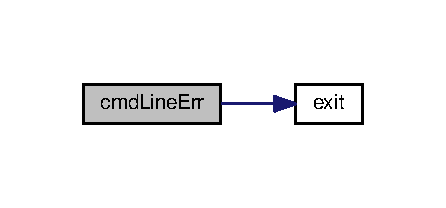
\includegraphics[width=214pt]{d2/d3d/common_2README_a2998a663efe6e91b3870e2bb7fba5504_cgraph}
\end{center}
\end{figure}


\hypertarget{common_2README_ad0cc7e68335dc54caa4465fe0ca45c21}{\index{common/\-R\-E\-A\-D\-M\-E@{common/\-R\-E\-A\-D\-M\-E}!err\-\_\-exit@{err\-\_\-exit}}
\index{err\-\_\-exit@{err\-\_\-exit}!common/README@{common/\-R\-E\-A\-D\-M\-E}}
\subsubsection[{err\-\_\-exit}]{\setlength{\rightskip}{0pt plus 5cm}$\ast$$\ast$$\ast$$\ast$$\ast$$\ast$$\ast$$\ast$$\ast$$\ast$$\ast$$\ast$$\ast$$\ast$$\ast$$\ast$$\ast$$\ast$$\ast$$\ast$$\ast$$\ast$$\ast$$\ast$$\ast$$\ast$$\ast$$\ast$ Calls which sets {\bf errno}$\ast$$\ast$$\ast$$\ast$$\ast$$\ast$$\ast$$\ast$$\ast$$\ast$$\ast$$\ast$$\ast$$\ast$$\ast$$\ast$$\ast$$\ast$$\ast$$\ast$$\ast$$\ast$$\ast$$\ast$$\ast$$\ast$$\ast$$\ast$ To diagnose {\bf errors} from system calls and {\bf library} we use err\-\_\-exit (
\begin{DoxyParamCaption}
{}
\end{DoxyParamCaption}
)}}\label{common_2README_ad0cc7e68335dc54caa4465fe0ca45c21}
\hypertarget{common_2README_ad83bc66851be4582ec97ba670a95fa0a}{\index{common/\-R\-E\-A\-D\-M\-E@{common/\-R\-E\-A\-D\-M\-E}!err\-\_\-exit@{err\-\_\-exit}}
\index{err\-\_\-exit@{err\-\_\-exit}!common/README@{common/\-R\-E\-A\-D\-M\-E}}
\subsubsection[{err\-\_\-exit}]{\setlength{\rightskip}{0pt plus 5cm}void err\-\_\-exit (
\begin{DoxyParamCaption}
\item[{const char $\ast$}]{format, }
\item[{}]{...}
\end{DoxyParamCaption}
)}}\label{common_2README_ad83bc66851be4582ec97ba670a95fa0a}


\-: Method to print the message with errno message, with \-\_\-exit. 

\begin{DoxyAuthor}{Author}
\-: Ravi Prasad (India) 
\end{DoxyAuthor}


Definition at line 122 of file error\-\_\-functions.\-c.



Here is the call graph for this function\-:
\nopagebreak
\begin{figure}[H]
\begin{center}
\leavevmode
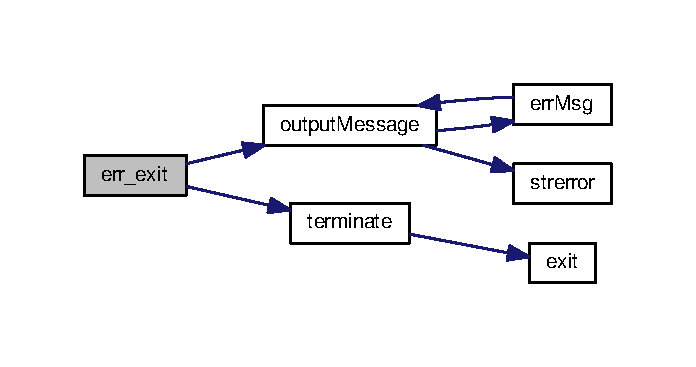
\includegraphics[width=334pt]{d2/d3d/common_2README_ad83bc66851be4582ec97ba670a95fa0a_cgraph}
\end{center}
\end{figure}


\hypertarget{common_2README_a68943fd8366445b15b2c72863bbc5b01}{\index{common/\-R\-E\-A\-D\-M\-E@{common/\-R\-E\-A\-D\-M\-E}!err\-Exit@{err\-Exit}}
\index{err\-Exit@{err\-Exit}!common/README@{common/\-R\-E\-A\-D\-M\-E}}
\subsubsection[{err\-Exit}]{\setlength{\rightskip}{0pt plus 5cm}$\ast$$\ast$$\ast$$\ast$$\ast$$\ast$$\ast$$\ast$$\ast$$\ast$$\ast$$\ast$$\ast$$\ast$$\ast$$\ast$$\ast$$\ast$$\ast$$\ast$$\ast$$\ast$$\ast$$\ast$$\ast$$\ast$$\ast$$\ast$ Calls which sets {\bf errno}$\ast$$\ast$$\ast$$\ast$$\ast$$\ast$$\ast$$\ast$$\ast$$\ast$$\ast$$\ast$$\ast$$\ast$$\ast$$\ast$$\ast$$\ast$$\ast$$\ast$$\ast$$\ast$$\ast$$\ast$$\ast$$\ast$$\ast$$\ast$ To diagnose {\bf errors} from system calls and {\bf library} we use err\-Exit (
\begin{DoxyParamCaption}
{}
\end{DoxyParamCaption}
)}}\label{common_2README_a68943fd8366445b15b2c72863bbc5b01}
\hypertarget{common_2README_a9353730adacb3417493e841dace8708b}{\index{common/\-R\-E\-A\-D\-M\-E@{common/\-R\-E\-A\-D\-M\-E}!err\-Exit@{err\-Exit}}
\index{err\-Exit@{err\-Exit}!common/README@{common/\-R\-E\-A\-D\-M\-E}}
\subsubsection[{err\-Exit}]{\setlength{\rightskip}{0pt plus 5cm}void err\-Exit (
\begin{DoxyParamCaption}
\item[{const char $\ast$}]{format, }
\item[{}]{...}
\end{DoxyParamCaption}
)}}\label{common_2README_a9353730adacb3417493e841dace8708b}


\-: Method to print the message with errno message, with exit. 

\begin{DoxyAuthor}{Author}
\-: Ravi Prasad (India) 
\end{DoxyAuthor}


Definition at line 106 of file error\-\_\-functions.\-c.



Here is the call graph for this function\-:
\nopagebreak
\begin{figure}[H]
\begin{center}
\leavevmode
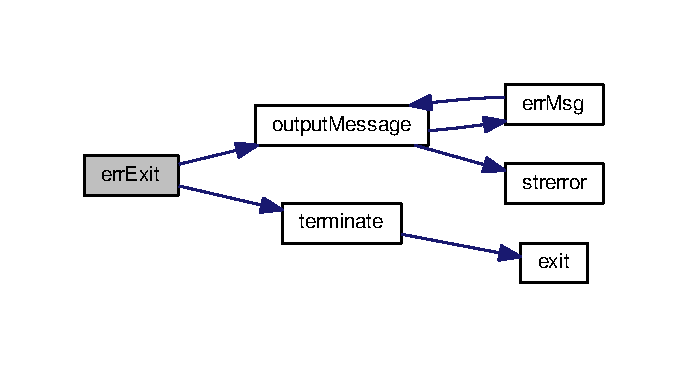
\includegraphics[width=330pt]{d2/d3d/common_2README_a9353730adacb3417493e841dace8708b_cgraph}
\end{center}
\end{figure}


\hypertarget{common_2README_a7c791eab42a732b614ef10956cc9b101}{\index{common/\-R\-E\-A\-D\-M\-E@{common/\-R\-E\-A\-D\-M\-E}!err\-Exit\-E\-N@{err\-Exit\-E\-N}}
\index{err\-Exit\-E\-N@{err\-Exit\-E\-N}!common/README@{common/\-R\-E\-A\-D\-M\-E}}
\subsubsection[{err\-Exit\-E\-N}]{\setlength{\rightskip}{0pt plus 5cm}except that a terminating newline character is automatically appended to {\bf the} output string The such as plus {\bf the} {\bf error} description as returned by but also terminates {\bf the} by calling but differs in two except that instead of printing {\bf the} {\bf error} text corresponding to {\bf the} current value of it prints {\bf the} text corresponding to {\bf the} {\bf error} we use err\-Exit\-E\-N (
\begin{DoxyParamCaption}
{}
\end{DoxyParamCaption}
)}}\label{common_2README_a7c791eab42a732b614ef10956cc9b101}
\hypertarget{common_2README_a6d6d5790ca5bffa970baeeefd8a28462}{\index{common/\-R\-E\-A\-D\-M\-E@{common/\-R\-E\-A\-D\-M\-E}!err\-Exit\-E\-N@{err\-Exit\-E\-N}}
\index{err\-Exit\-E\-N@{err\-Exit\-E\-N}!common/README@{common/\-R\-E\-A\-D\-M\-E}}
\subsubsection[{err\-Exit\-E\-N}]{\setlength{\rightskip}{0pt plus 5cm}void err\-Exit\-E\-N (
\begin{DoxyParamCaption}
\item[{int}]{err\-Num, }
\item[{const char $\ast$}]{format, }
\item[{}]{...}
\end{DoxyParamCaption}
)}}\label{common_2README_a6d6d5790ca5bffa970baeeefd8a28462}


\-: Method to print the message with errno message, with exit call. 

\begin{DoxyAuthor}{Author}
\-: Ravi Prasad (India) 
\end{DoxyAuthor}


Definition at line 138 of file error\-\_\-functions.\-c.



Here is the call graph for this function\-:
\nopagebreak
\begin{figure}[H]
\begin{center}
\leavevmode
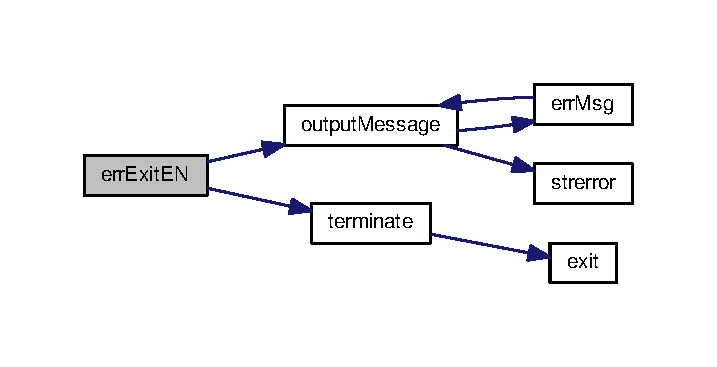
\includegraphics[width=344pt]{d2/d3d/common_2README_a6d6d5790ca5bffa970baeeefd8a28462_cgraph}
\end{center}
\end{figure}


\hypertarget{common_2README_aaa5f75c9c764c204bf342e6b6cc969f6}{\index{common/\-R\-E\-A\-D\-M\-E@{common/\-R\-E\-A\-D\-M\-E}!err\-Exit\-E\-N@{err\-Exit\-E\-N}}
\index{err\-Exit\-E\-N@{err\-Exit\-E\-N}!common/README@{common/\-R\-E\-A\-D\-M\-E}}
\subsubsection[{err\-Exit\-E\-N}]{\setlength{\rightskip}{0pt plus 5cm}except that a terminating newline character is automatically appended to {\bf the} output string The such as plus {\bf the} {\bf error} description as returned by but also terminates {\bf the} by calling but differs in two except that instead of printing {\bf the} {\bf error} text corresponding to {\bf the} current value of it prints {\bf the} text corresponding to {\bf the} {\bf error} we use which return –1 on {\bf the} P\-O\-S\-I\-X threads {\bf functions} diagnose an {\bf error} by returning an {\bf error} {\bf number} (i.\-e., a positive {\bf number} of {\bf the} type normally placed in {\bf errno}) as their function result. (The P\-O\-S\-I\-X threads {\bf functions} return 0 on success.) Example err\-Exit\-E\-N (
\begin{DoxyParamCaption}
\item[{s}]{, }
\item[{\char`\"{}pthread\-\_\-create\char`\"{}}]{}
\end{DoxyParamCaption}
)}}\label{common_2README_aaa5f75c9c764c204bf342e6b6cc969f6}
\hypertarget{common_2README_a83413e40798cc613af12fa88a21035a5}{\index{common/\-R\-E\-A\-D\-M\-E@{common/\-R\-E\-A\-D\-M\-E}!err\-Msg@{err\-Msg}}
\index{err\-Msg@{err\-Msg}!common/README@{common/\-R\-E\-A\-D\-M\-E}}
\subsubsection[{err\-Msg}]{\setlength{\rightskip}{0pt plus 5cm}except that a terminating newline character is automatically appended to {\bf the} output string The err\-Msg (
\begin{DoxyParamCaption}
{}
\end{DoxyParamCaption}
)}}\label{common_2README_a83413e40798cc613af12fa88a21035a5}
\hypertarget{common_2README_a85c39bfe84eed5e1d7dae87fb0018669}{\index{common/\-R\-E\-A\-D\-M\-E@{common/\-R\-E\-A\-D\-M\-E}!exit@{exit}}
\index{exit@{exit}!common/README@{common/\-R\-E\-A\-D\-M\-E}}
\subsubsection[{exit}]{\setlength{\rightskip}{0pt plus 5cm}except that a terminating newline character is automatically appended to {\bf the} output string The such as plus {\bf the} {\bf error} description as returned by but also terminates {\bf the} by calling exit (
\begin{DoxyParamCaption}
{}
\end{DoxyParamCaption}
)}}\label{common_2README_a85c39bfe84eed5e1d7dae87fb0018669}


Here is the caller graph for this function\-:
\nopagebreak
\begin{figure}[H]
\begin{center}
\leavevmode
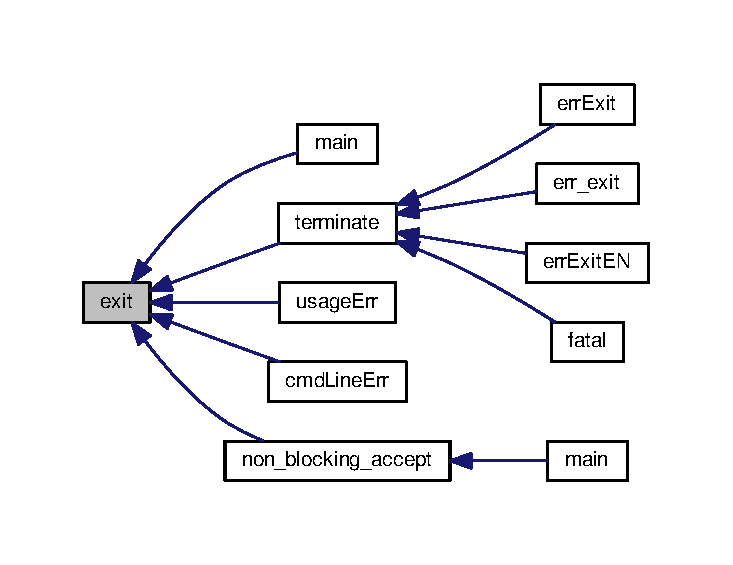
\includegraphics[width=350pt]{d2/d3d/common_2README_a85c39bfe84eed5e1d7dae87fb0018669_icgraph}
\end{center}
\end{figure}


\hypertarget{common_2README_ae688a97aa2b3eb3a27322a140be60049}{\index{common/\-R\-E\-A\-D\-M\-E@{common/\-R\-E\-A\-D\-M\-E}!fatal@{fatal}}
\index{fatal@{fatal}!common/README@{common/\-R\-E\-A\-D\-M\-E}}
\subsubsection[{fatal}]{\setlength{\rightskip}{0pt plus 5cm}$\ast$$\ast$$\ast$$\ast$$\ast$$\ast$$\ast$$\ast$$\ast$$\ast$$\ast$$\ast$$\ast$$\ast$$\ast$$\ast$$\ast$$\ast$$\ast$$\ast$$\ast$$\ast$$\ast$$\ast$$\ast$$\ast$$\ast$$\ast$$\ast$$\ast$$\ast$$\ast$$\ast$$\ast$$\ast$$\ast$$\ast$$\ast$$\ast$$\ast$$\ast$ Calls which doesn t sets {\bf errno}$\ast$$\ast$$\ast$$\ast$$\ast$$\ast$$\ast$$\ast$$\ast$$\ast$$\ast$$\ast$$\ast$$\ast$$\ast$$\ast$$\ast$$\ast$$\ast$$\ast$$\ast$$\ast$$\ast$$\ast$$\ast$$\ast$$\ast$$\ast$$\ast$$\ast$$\ast$$\ast$$\ast$$\ast$$\ast$$\ast$$\ast$$\ast$$\ast$$\ast$$\ast$ To diagnose other types of we use fatal (
\begin{DoxyParamCaption}
{}
\end{DoxyParamCaption}
)}}\label{common_2README_ae688a97aa2b3eb3a27322a140be60049}
\hypertarget{common_2README_aba79e3975c1b7da6e77c2f4b561603ae}{\index{common/\-R\-E\-A\-D\-M\-E@{common/\-R\-E\-A\-D\-M\-E}!number@{number}}
\index{number@{number}!common/README@{common/\-R\-E\-A\-D\-M\-E}}
\subsubsection[{number}]{\setlength{\rightskip}{0pt plus 5cm}except that a terminating newline character is automatically appended to {\bf the} output string The such as plus {\bf the} {\bf error} description as returned by but also terminates {\bf the} by calling but differs in two except that instead of printing {\bf the} {\bf error} text corresponding to {\bf the} current value of it prints {\bf the} text corresponding to {\bf the} {\bf error} number (
\begin{DoxyParamCaption}
\item[{thus}]{, }
\item[{{\bf the} E\-N}]{suffix}
\end{DoxyParamCaption}
)}}\label{common_2README_aba79e3975c1b7da6e77c2f4b561603ae}
\hypertarget{common_2README_ae46f6c5c5729768631dc5ff84e16d52b}{\index{common/\-R\-E\-A\-D\-M\-E@{common/\-R\-E\-A\-D\-M\-E}!printf@{printf}}
\index{printf@{printf}!common/README@{common/\-R\-E\-A\-D\-M\-E}}
\subsubsection[{printf}]{\setlength{\rightskip}{0pt plus 5cm}including {\bf errors} from {\bf library} {\bf functions} that don’t set {\bf errno} Its argument list is {\bf the} same as for printf (
\begin{DoxyParamCaption}
{}
\end{DoxyParamCaption}
)}}\label{common_2README_ae46f6c5c5729768631dc5ff84e16d52b}


Here is the caller graph for this function\-:
\nopagebreak
\begin{figure}[H]
\begin{center}
\leavevmode
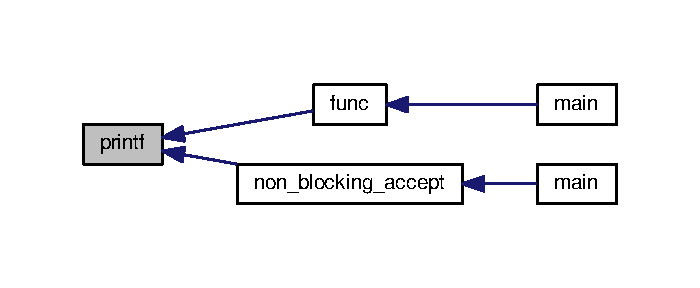
\includegraphics[width=336pt]{d2/d3d/common_2README_ae46f6c5c5729768631dc5ff84e16d52b_icgraph}
\end{center}
\end{figure}


\hypertarget{common_2README_af3164892dd3bd1beaa3a2b70e01edcd9}{\index{common/\-R\-E\-A\-D\-M\-E@{common/\-R\-E\-A\-D\-M\-E}!strerror@{strerror}}
\index{strerror@{strerror}!common/README@{common/\-R\-E\-A\-D\-M\-E}}
\subsubsection[{strerror}]{\setlength{\rightskip}{0pt plus 5cm}except that a terminating newline character is automatically appended to {\bf the} output string The such as plus {\bf the} {\bf error} description as returned by strerror (
\begin{DoxyParamCaption}
{}
\end{DoxyParamCaption}
)}}\label{common_2README_af3164892dd3bd1beaa3a2b70e01edcd9}


Here is the caller graph for this function\-:
\nopagebreak
\begin{figure}[H]
\begin{center}
\leavevmode
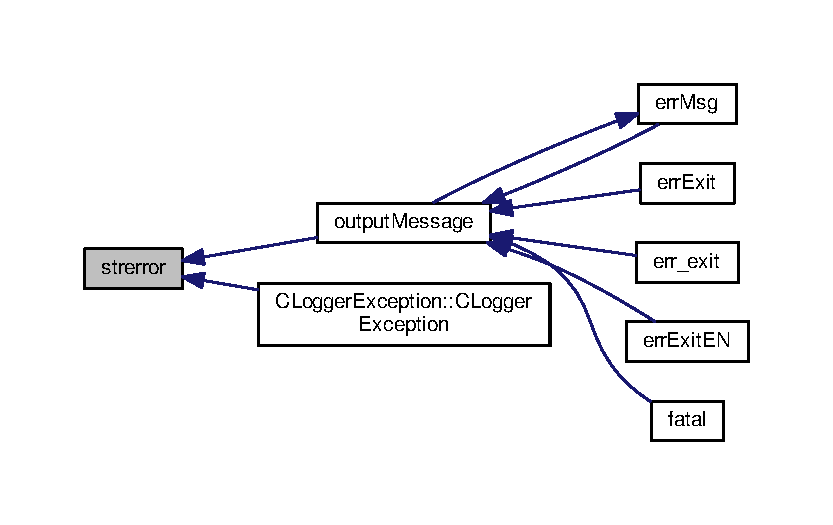
\includegraphics[width=350pt]{d2/d3d/common_2README_af3164892dd3bd1beaa3a2b70e01edcd9_icgraph}
\end{center}
\end{figure}


\hypertarget{common_2README_aff916c132f7e6f0b0dec6d7c28ee2573}{\index{common/\-R\-E\-A\-D\-M\-E@{common/\-R\-E\-A\-D\-M\-E}!usage\-Err@{usage\-Err}}
\index{usage\-Err@{usage\-Err}!common/README@{common/\-R\-E\-A\-D\-M\-E}}
\subsubsection[{usage\-Err}]{\setlength{\rightskip}{0pt plus 5cm}$\ast$$\ast$$\ast$$\ast$$\ast$$\ast$$\ast$$\ast$$\ast$$\ast$$\ast$$\ast$$\ast$$\ast$$\ast$$\ast$$\ast$$\ast$$\ast$$\ast$$\ast$$\ast$$\ast$$\ast$$\ast$$\ast$$\ast$$\ast$$\ast$$\ast$$\ast$$\ast$$\ast$$\ast$$\ast$$\ast$$\ast$$\ast$$\ast$$\ast$$\ast$ Calls which doesn t sets {\bf errno}$\ast$$\ast$$\ast$$\ast$$\ast$$\ast$$\ast$$\ast$$\ast$$\ast$$\ast$$\ast$$\ast$$\ast$$\ast$$\ast$$\ast$$\ast$$\ast$$\ast$$\ast$$\ast$$\ast$$\ast$$\ast$$\ast$$\ast$$\ast$$\ast$$\ast$$\ast$$\ast$$\ast$$\ast$$\ast$$\ast$$\ast$$\ast$$\ast$$\ast$$\ast$ To diagnose other types of we use usage\-Err (
\begin{DoxyParamCaption}
{}
\end{DoxyParamCaption}
)}}\label{common_2README_aff916c132f7e6f0b0dec6d7c28ee2573}
\hypertarget{common_2README_a0c81140d074e6630634e05e7ca437390}{\index{common/\-R\-E\-A\-D\-M\-E@{common/\-R\-E\-A\-D\-M\-E}!usage\-Err@{usage\-Err}}
\index{usage\-Err@{usage\-Err}!common/README@{common/\-R\-E\-A\-D\-M\-E}}
\subsubsection[{usage\-Err}]{\setlength{\rightskip}{0pt plus 5cm}void usage\-Err (
\begin{DoxyParamCaption}
\item[{const char $\ast$}]{format, }
\item[{}]{...}
\end{DoxyParamCaption}
)}}\label{common_2README_a0c81140d074e6630634e05e7ca437390}


\-: Method to print the uses error. 

\begin{DoxyAuthor}{Author}
\-: Ravi Prasad (India) 
\end{DoxyAuthor}


Definition at line 169 of file error\-\_\-functions.\-c.



Here is the call graph for this function\-:
\nopagebreak
\begin{figure}[H]
\begin{center}
\leavevmode
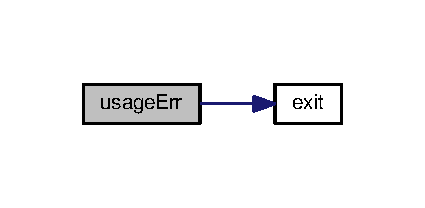
\includegraphics[width=204pt]{d2/d3d/common_2README_a0c81140d074e6630634e05e7ca437390_cgraph}
\end{center}
\end{figure}




\subsection{Variable Documentation}
\hypertarget{common_2README_a9f655c76c94b7fe5fa4714a077ef4d7e}{\index{common/\-R\-E\-A\-D\-M\-E@{common/\-R\-E\-A\-D\-M\-E}!E\-P\-E\-R\-M@{E\-P\-E\-R\-M}}
\index{E\-P\-E\-R\-M@{E\-P\-E\-R\-M}!common/README@{common/\-R\-E\-A\-D\-M\-E}}
\subsubsection[{E\-P\-E\-R\-M}]{\setlength{\rightskip}{0pt plus 5cm}except that a terminating newline character is automatically appended to {\bf the} output string The such as E\-P\-E\-R\-M}}\label{common_2README_a9f655c76c94b7fe5fa4714a077ef4d7e}


Definition at line 18 of file R\-E\-A\-D\-M\-E.

\hypertarget{common_2README_afe75ee0c7e5a90ba6bb38426ea69b996}{\index{common/\-R\-E\-A\-D\-M\-E@{common/\-R\-E\-A\-D\-M\-E}!errno@{errno}}
\index{errno@{errno}!common/README@{common/\-R\-E\-A\-D\-M\-E}}
\subsubsection[{errno}]{\setlength{\rightskip}{0pt plus 5cm}except that a terminating newline character is automatically appended to {\bf the} output string The such as plus {\bf the} {\bf error} description as returned by but also terminates {\bf the} by calling but differs in two except that instead of printing {\bf the} {\bf error} text corresponding to {\bf the} current value of errno}}\label{common_2README_afe75ee0c7e5a90ba6bb38426ea69b996}


Definition at line 28 of file R\-E\-A\-D\-M\-E.

\hypertarget{common_2README_a80171b13188418b4328f9247d3aff3d2}{\index{common/\-R\-E\-A\-D\-M\-E@{common/\-R\-E\-A\-D\-M\-E}!error@{error}}
\index{error@{error}!common/README@{common/\-R\-E\-A\-D\-M\-E}}
\subsubsection[{error}]{\setlength{\rightskip}{0pt plus 5cm}except that a terminating newline character is automatically appended to {\bf the} output string The such as plus {\bf the} error description as returned by but also terminates {\bf the} by calling but differs in two except that instead of printing {\bf the} error text corresponding to {\bf the} current value of it prints {\bf the} text corresponding to {\bf the} error we use which return –1 on error}}\label{common_2README_a80171b13188418b4328f9247d3aff3d2}


Definition at line 33 of file R\-E\-A\-D\-M\-E.

\hypertarget{common_2README_a9912daeb8cc621a6ee8e1d24ebdbe601}{\index{common/\-R\-E\-A\-D\-M\-E@{common/\-R\-E\-A\-D\-M\-E}!errors@{errors}}
\index{errors@{errors}!common/README@{common/\-R\-E\-A\-D\-M\-E}}
\subsubsection[{errors}]{\setlength{\rightskip}{0pt plus 5cm}$\ast$$\ast$$\ast$$\ast$$\ast$$\ast$$\ast$$\ast$$\ast$$\ast$$\ast$$\ast$$\ast$$\ast$$\ast$$\ast$$\ast$$\ast$$\ast$$\ast$$\ast$$\ast$$\ast$$\ast$$\ast$$\ast$$\ast$$\ast$$\ast$$\ast$$\ast$$\ast$$\ast$$\ast$$\ast$$\ast$$\ast$$\ast$$\ast$$\ast$$\ast$ Calls which doesn t sets {\bf errno}$\ast$$\ast$$\ast$$\ast$$\ast$$\ast$$\ast$$\ast$$\ast$$\ast$$\ast$$\ast$$\ast$$\ast$$\ast$$\ast$$\ast$$\ast$$\ast$$\ast$$\ast$$\ast$$\ast$$\ast$$\ast$$\ast$$\ast$$\ast$$\ast$$\ast$$\ast$$\ast$$\ast$$\ast$$\ast$$\ast$$\ast$$\ast$$\ast$$\ast$$\ast$ To diagnose other types of errors}}\label{common_2README_a9912daeb8cc621a6ee8e1d24ebdbe601}


Definition at line 46 of file R\-E\-A\-D\-M\-E.

\hypertarget{common_2README_a853571ba73c010b99ff2788a0cfe4395}{\index{common/\-R\-E\-A\-D\-M\-E@{common/\-R\-E\-A\-D\-M\-E}!functions@{functions}}
\index{functions@{functions}!common/README@{common/\-R\-E\-A\-D\-M\-E}}
\subsubsection[{functions}]{\setlength{\rightskip}{0pt plus 5cm}$\ast$$\ast$$\ast$$\ast$$\ast$$\ast$$\ast$$\ast$$\ast$$\ast$$\ast$$\ast$$\ast$$\ast$$\ast$$\ast$$\ast$$\ast$$\ast$$\ast$$\ast$$\ast$$\ast$$\ast$$\ast$$\ast$$\ast$$\ast$ Calls which sets {\bf errno}$\ast$$\ast$$\ast$$\ast$$\ast$$\ast$$\ast$$\ast$$\ast$$\ast$$\ast$$\ast$$\ast$$\ast$$\ast$$\ast$$\ast$$\ast$$\ast$$\ast$$\ast$$\ast$$\ast$$\ast$$\ast$$\ast$$\ast$$\ast$ To diagnose {\bf errors} from system calls and {\bf library} functions}}\label{common_2README_a853571ba73c010b99ff2788a0cfe4395}


Definition at line 4 of file R\-E\-A\-D\-M\-E.

\hypertarget{common_2README_a2648c031e7768d2922f9bceca11215d9}{\index{common/\-R\-E\-A\-D\-M\-E@{common/\-R\-E\-A\-D\-M\-E}!program@{program}}
\index{program@{program}!common/README@{common/\-R\-E\-A\-D\-M\-E}}
\subsubsection[{program}]{\setlength{\rightskip}{0pt plus 5cm}except that a terminating newline character is automatically appended to {\bf the} output string The such as plus {\bf the} {\bf error} description as returned by but also terminates {\bf the} program}}\label{common_2README_a2648c031e7768d2922f9bceca11215d9}


Definition at line 21 of file R\-E\-A\-D\-M\-E.

\hypertarget{common_2README_a33a4706d30ee60d6fc7d0c4b387dc3b9}{\index{common/\-R\-E\-A\-D\-M\-E@{common/\-R\-E\-A\-D\-M\-E}!respects@{respects}}
\index{respects@{respects}!common/README@{common/\-R\-E\-A\-D\-M\-E}}
\subsubsection[{respects}]{\setlength{\rightskip}{0pt plus 5cm}except that a terminating newline character is automatically appended to {\bf the} output string The such as plus {\bf the} {\bf error} description as returned by but also terminates {\bf the} by calling but differs in two respects}}\label{common_2README_a33a4706d30ee60d6fc7d0c4b387dc3b9}


Definition at line 28 of file R\-E\-A\-D\-M\-E.


\hypertarget{logging_2README}{\section{logging/\-R\-E\-A\-D\-M\-E File Reference}
\label{logging_2README}\index{logging/\-R\-E\-A\-D\-M\-E@{logging/\-R\-E\-A\-D\-M\-E}}
}

\hypertarget{README}{\section{R\-E\-A\-D\-M\-E File Reference}
\label{README}\index{R\-E\-A\-D\-M\-E@{R\-E\-A\-D\-M\-E}}
}
\subsection*{Functions}
\begin{DoxyCompactItemize}
\item 
Copyright Ravi \hyperlink{README_acbcec0b507f57bc6fea73bd91bc0323f}{Prasad} (India)-\/-\/-\/-\/-\/-\/-\/-\/-\/-\/-\/-\/-\/-\/-\/-\/-\/-\/-\/-\/-\/-\/-\/-\/-\/-\/-\/-\/-\/-\/-\/-\/-\/-\/-\/-\/-\/-\/-\/About-\/-\/-\/-\/-\/-\/-\/-\/-\/-\/-\/-\/-\/-\/-\/-\/-\/-\/-\/-\/-\/-\/-\/-\/-\/-\/-\/-\/-\/-\/-\/-\/-\/-\/-\/-\/-\/-\/-\/-\/This repo servers two things.\-1.\-Deployment of posix socket \hyperlink{ClientServer_2server_2Makefile_a1f477410360bd4832116581b9934ab71}{library}(blocking and non blocking) 2.Uses of \hyperlink{ClientServer_2server_2Makefile_a09c6b60bb7451f9136e25140ffdff6bd}{the} socket \hyperlink{ClientServer_2server_2Makefile_a1f477410360bd4832116581b9934ab71}{library} with \hyperlink{ClientServer_2server_2Makefile_a09c6b60bb7451f9136e25140ffdff6bd}{the} Cliet\-Sever Module.\-Uses-\/-\/-\/-\/-\/-\/-\/-\/-\/-\/-\/-\/-\/-\/-\/-\/-\/-\/-\/-\/-\/-\/-\/-\/-\/-\/-\/-\/-\/-\/-\/-\/-\/-\/-\/-\/-\/-\/1.git clone$<$ This repo $>$ 2.go to Socket\-Library.\-3.\-Run make.\-After Make
\end{DoxyCompactItemize}
\subsection*{Variables}
\begin{DoxyCompactItemize}
\item 
Copyright Ravi it will create \\*
client and server exe as \\*
follows For \hyperlink{README_acced105257a718491134c7cae002d48a}{R\-H\-E\-L}
\item 
Copyright Ravi it will create \\*
client and server exe as \\*
follows For \hyperlink{README_abec6047e55a548b2b675ef60ec1a1ff0}{C\-E\-N\-T\-O\-S}
\item 
Copyright Ravi it will create \\*
client and server exe as \\*
follows For B\-S\-D Socket\-Library \\*
Client\-Server client Linux \\*
client Socket\-Library \\*
Client\-Server server Linux \\*
server Running \hyperlink{ClientServer_2server_2Makefile_a09c6b60bb7451f9136e25140ffdff6bd}{the} client and \\*
server From Server \hyperlink{README_a38037a5a8331147623d2579e11a55ddc}{Host}
\end{DoxyCompactItemize}


\subsection{Function Documentation}
\hypertarget{README_acbcec0b507f57bc6fea73bd91bc0323f}{\index{R\-E\-A\-D\-M\-E@{R\-E\-A\-D\-M\-E}!Prasad@{Prasad}}
\index{Prasad@{Prasad}!README@{R\-E\-A\-D\-M\-E}}
\subsubsection[{Prasad}]{\setlength{\rightskip}{0pt plus 5cm}Copyright Ravi Prasad (
\begin{DoxyParamCaption}
\item[{India}]{}
\end{DoxyParamCaption}
)}}\label{README_acbcec0b507f57bc6fea73bd91bc0323f}


\subsection{Variable Documentation}
\hypertarget{README_abec6047e55a548b2b675ef60ec1a1ff0}{\index{R\-E\-A\-D\-M\-E@{R\-E\-A\-D\-M\-E}!C\-E\-N\-T\-O\-S@{C\-E\-N\-T\-O\-S}}
\index{C\-E\-N\-T\-O\-S@{C\-E\-N\-T\-O\-S}!README@{R\-E\-A\-D\-M\-E}}
\subsubsection[{C\-E\-N\-T\-O\-S}]{\setlength{\rightskip}{0pt plus 5cm}Copyright Ravi it will create client and server exe as follows For C\-E\-N\-T\-O\-S}}\label{README_abec6047e55a548b2b675ef60ec1a1ff0}


Definition at line 17 of file R\-E\-A\-D\-M\-E.

\hypertarget{README_a38037a5a8331147623d2579e11a55ddc}{\index{R\-E\-A\-D\-M\-E@{R\-E\-A\-D\-M\-E}!Host@{Host}}
\index{Host@{Host}!README@{R\-E\-A\-D\-M\-E}}
\subsubsection[{Host}]{\setlength{\rightskip}{0pt plus 5cm}Copyright Ravi it will create client and server exe as follows For B\-S\-D Socket\-Library Client\-Server client Linux client Socket\-Library Client\-Server server Linux server Running {\bf the} client and server From Server server will reply {\bf the} same message From Client server will reply {\bf the} same message From Client server will reply {\bf the} same message From Client Host}}\label{README_a38037a5a8331147623d2579e11a55ddc}


Definition at line 17 of file R\-E\-A\-D\-M\-E.

\hypertarget{README_acced105257a718491134c7cae002d48a}{\index{R\-E\-A\-D\-M\-E@{R\-E\-A\-D\-M\-E}!R\-H\-E\-L@{R\-H\-E\-L}}
\index{R\-H\-E\-L@{R\-H\-E\-L}!README@{R\-E\-A\-D\-M\-E}}
\subsubsection[{R\-H\-E\-L}]{\setlength{\rightskip}{0pt plus 5cm}Copyright Ravi it will create client and server exe as follows For R\-H\-E\-L}}\label{README_acced105257a718491134c7cae002d48a}


Definition at line 17 of file R\-E\-A\-D\-M\-E.


\hypertarget{tcpSocket_2README}{\section{tcp\-Socket/\-R\-E\-A\-D\-M\-E File Reference}
\label{tcpSocket_2README}\index{tcp\-Socket/\-R\-E\-A\-D\-M\-E@{tcp\-Socket/\-R\-E\-A\-D\-M\-E}}
}
\subsection*{Variables}
\begin{DoxyCompactItemize}
\item 
Server Design \hyperlink{tcpSocket_2README_a3652bdf2b1d82505530a3f0fae48505c}{Iterative}
\item 
Server Design processing that \\*
client s request \hyperlink{tcpSocket_2README_a25176105e88a72b92d4d66dccbccc2dc}{completly}
\item 
Server Design processing that \\*
client s request before \\*
roceceeding to \hyperlink{ClientServer_2server_2Makefile_a09c6b60bb7451f9136e25140ffdff6bd}{the} next client \hyperlink{tcpSocket_2README_a47da67c2ce0f5106f4d7c6b944cfa68a}{Cocurent}
\end{DoxyCompactItemize}


\subsection{Variable Documentation}
\hypertarget{tcpSocket_2README_a47da67c2ce0f5106f4d7c6b944cfa68a}{\index{tcp\-Socket/\-R\-E\-A\-D\-M\-E@{tcp\-Socket/\-R\-E\-A\-D\-M\-E}!Cocurent@{Cocurent}}
\index{Cocurent@{Cocurent}!tcpSocket/README@{tcp\-Socket/\-R\-E\-A\-D\-M\-E}}
\subsubsection[{Cocurent}]{\setlength{\rightskip}{0pt plus 5cm}Server Design processing that client s request before roceceeding to {\bf the} next client Cocurent}}\label{tcpSocket_2README_a47da67c2ce0f5106f4d7c6b944cfa68a}


Definition at line 4 of file R\-E\-A\-D\-M\-E.

\hypertarget{tcpSocket_2README_a25176105e88a72b92d4d66dccbccc2dc}{\index{tcp\-Socket/\-R\-E\-A\-D\-M\-E@{tcp\-Socket/\-R\-E\-A\-D\-M\-E}!completly@{completly}}
\index{completly@{completly}!tcpSocket/README@{tcp\-Socket/\-R\-E\-A\-D\-M\-E}}
\subsubsection[{completly}]{\setlength{\rightskip}{0pt plus 5cm}Server Design processing that client s request completly}}\label{tcpSocket_2README_a25176105e88a72b92d4d66dccbccc2dc}


Definition at line 4 of file R\-E\-A\-D\-M\-E.

\hypertarget{tcpSocket_2README_a3652bdf2b1d82505530a3f0fae48505c}{\index{tcp\-Socket/\-R\-E\-A\-D\-M\-E@{tcp\-Socket/\-R\-E\-A\-D\-M\-E}!Iterative@{Iterative}}
\index{Iterative@{Iterative}!tcpSocket/README@{tcp\-Socket/\-R\-E\-A\-D\-M\-E}}
\subsubsection[{Iterative}]{\setlength{\rightskip}{0pt plus 5cm}Server Design Iterative}}\label{tcpSocket_2README_a3652bdf2b1d82505530a3f0fae48505c}


Definition at line 4 of file R\-E\-A\-D\-M\-E.


\hypertarget{error__functions_8c}{\section{common/source/error\-\_\-functions.c File Reference}
\label{error__functions_8c}\index{common/source/error\-\_\-functions.\-c@{common/source/error\-\_\-functions.\-c}}
}
{\ttfamily \#include $<$stdarg.\-h$>$}\\*
{\ttfamily \#include $<$error\-\_\-functions.\-h$>$}\\*
{\ttfamily \#include $<$get\-\_\-num.\-h$>$}\\*
{\ttfamily \#include \char`\"{}tlpi\-\_\-hdr.\-h\char`\"{}}\\*
Include dependency graph for error\-\_\-functions.\-c\-:
\nopagebreak
\begin{figure}[H]
\begin{center}
\leavevmode
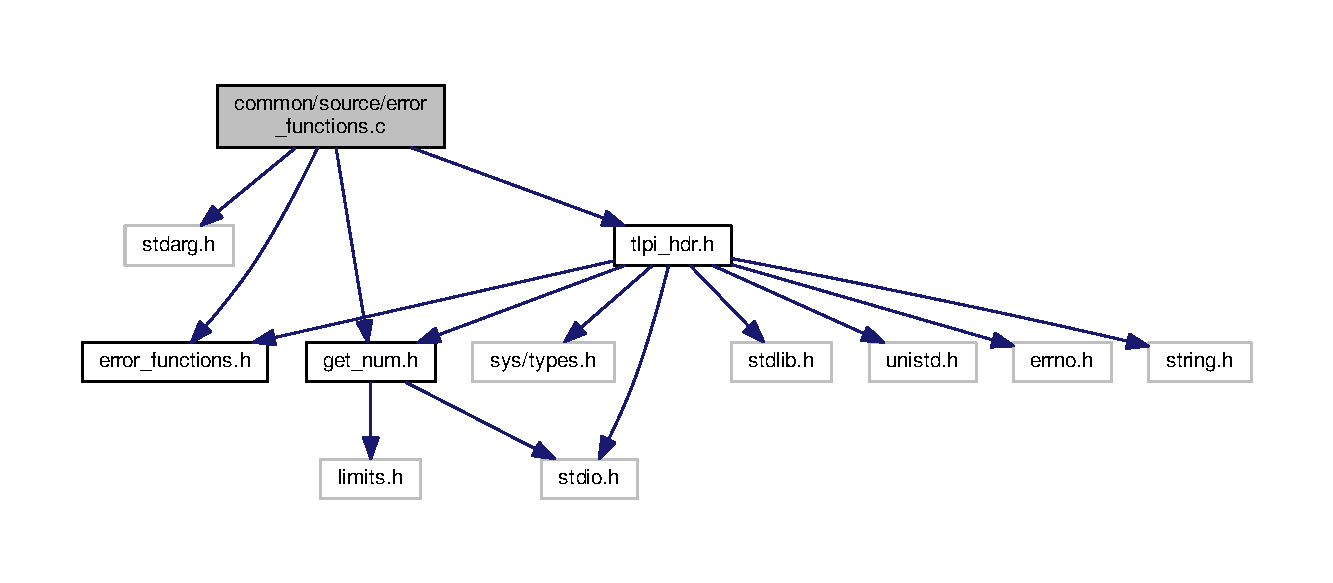
\includegraphics[width=350pt]{d8/dde/error__functions_8c__incl}
\end{center}
\end{figure}
\subsection*{Macros}
\begin{DoxyCompactItemize}
\item 
\#define \hyperlink{error__functions_8c_a6c7cd32e1bac137f05e4a752b4ad10af}{B\-U\-F\-F\-\_\-\-S\-I\-Z\-E}~256
\end{DoxyCompactItemize}
\subsection*{Functions}
\begin{DoxyCompactItemize}
\item 
static void \hyperlink{error__functions_8c_ad0aaa18a5967e8ea284b980da0029f58}{terminate} (\hyperlink{tlpi__hdr_8h_aec7e62084419d7857ae740a4c68241cf}{B\-O\-O\-L\-E\-A\-N} use\-Exit)
\begin{DoxyCompactList}\small\item\em \-: Note\-: Difference between \hyperlink{common_2README_a85c39bfe84eed5e1d7dae87fb0018669}{exit()} and \-\_\-exit() \end{DoxyCompactList}\item 
static void \hyperlink{error__functions_8c_accffbc65d0a3df9ae8a527062ffddd05}{output\-Message} (\hyperlink{tlpi__hdr_8h_aec7e62084419d7857ae740a4c68241cf}{B\-O\-O\-L\-E\-A\-N} use\-Err\-No, int err, \hyperlink{tlpi__hdr_8h_aec7e62084419d7857ae740a4c68241cf}{B\-O\-O\-L\-E\-A\-N} flush\-Buffer, const char $\ast$format, va\-\_\-list arg\-List)
\begin{DoxyCompactList}\small\item\em \-: Method to print the message with or without errorno message. \end{DoxyCompactList}\item 
void \hyperlink{error__functions_8c_a46c1ae408432a2c70da4402236454a5f}{err\-Msg} (const char $\ast$format,...)
\begin{DoxyCompactList}\small\item\em \-: Method to print the message with errno message, without exit or \-\_\-exit call. \end{DoxyCompactList}\item 
void \hyperlink{error__functions_8c_a9353730adacb3417493e841dace8708b}{err\-Exit} (const char $\ast$format,...)
\begin{DoxyCompactList}\small\item\em \-: Method to print the message with errno message, with exit. \end{DoxyCompactList}\item 
void \hyperlink{error__functions_8c_ad83bc66851be4582ec97ba670a95fa0a}{err\-\_\-exit} (const char $\ast$format,...)
\begin{DoxyCompactList}\small\item\em \-: Method to print the message with errno message, with \-\_\-exit. \end{DoxyCompactList}\item 
void \hyperlink{error__functions_8c_a88444cb888856a4241c156ae704e76de}{err\-Exit\-E\-N} (int err\-Num, const char $\ast$format,...)
\begin{DoxyCompactList}\small\item\em \-: Method to print the message with errno message, with exit call. \end{DoxyCompactList}\item 
void \hyperlink{error__functions_8c_abdee3dc73ec124f69d84a83af3ea90ce}{fatal} (const char $\ast$format,...)
\begin{DoxyCompactList}\small\item\em \-: Method to print the message with errno message, with \-\_\-exit call. \end{DoxyCompactList}\item 
void \hyperlink{error__functions_8c_a0c81140d074e6630634e05e7ca437390}{usage\-Err} (const char $\ast$format,...)
\begin{DoxyCompactList}\small\item\em \-: Method to print the uses error. \end{DoxyCompactList}\item 
void \hyperlink{error__functions_8c_a2998a663efe6e91b3870e2bb7fba5504}{cmd\-Line\-Err} (const char $\ast$format,...)
\begin{DoxyCompactList}\small\item\em \-: Method to print the command line argument error. \end{DoxyCompactList}\end{DoxyCompactItemize}


\subsection{Macro Definition Documentation}
\hypertarget{error__functions_8c_a6c7cd32e1bac137f05e4a752b4ad10af}{\index{error\-\_\-functions.\-c@{error\-\_\-functions.\-c}!B\-U\-F\-F\-\_\-\-S\-I\-Z\-E@{B\-U\-F\-F\-\_\-\-S\-I\-Z\-E}}
\index{B\-U\-F\-F\-\_\-\-S\-I\-Z\-E@{B\-U\-F\-F\-\_\-\-S\-I\-Z\-E}!error_functions.c@{error\-\_\-functions.\-c}}
\subsubsection[{B\-U\-F\-F\-\_\-\-S\-I\-Z\-E}]{\setlength{\rightskip}{0pt plus 5cm}\#define B\-U\-F\-F\-\_\-\-S\-I\-Z\-E~256}}\label{error__functions_8c_a6c7cd32e1bac137f05e4a752b4ad10af}


Definition at line 5 of file error\-\_\-functions.\-c.



\subsection{Function Documentation}
\hypertarget{error__functions_8c_a2998a663efe6e91b3870e2bb7fba5504}{\index{error\-\_\-functions.\-c@{error\-\_\-functions.\-c}!cmd\-Line\-Err@{cmd\-Line\-Err}}
\index{cmd\-Line\-Err@{cmd\-Line\-Err}!error_functions.c@{error\-\_\-functions.\-c}}
\subsubsection[{cmd\-Line\-Err}]{\setlength{\rightskip}{0pt plus 5cm}void cmd\-Line\-Err (
\begin{DoxyParamCaption}
\item[{const char $\ast$}]{format, }
\item[{}]{...}
\end{DoxyParamCaption}
)}}\label{error__functions_8c_a2998a663efe6e91b3870e2bb7fba5504}


\-: Method to print the command line argument error. 

\begin{DoxyAuthor}{Author}
\-: Ravi Prasad (India) 
\end{DoxyAuthor}


Definition at line 188 of file error\-\_\-functions.\-c.



Here is the call graph for this function\-:
\nopagebreak
\begin{figure}[H]
\begin{center}
\leavevmode
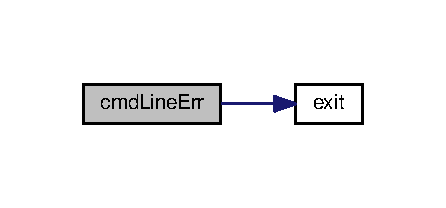
\includegraphics[width=214pt]{dd/d35/error__functions_8c_a2998a663efe6e91b3870e2bb7fba5504_cgraph}
\end{center}
\end{figure}


\hypertarget{error__functions_8c_ad83bc66851be4582ec97ba670a95fa0a}{\index{error\-\_\-functions.\-c@{error\-\_\-functions.\-c}!err\-\_\-exit@{err\-\_\-exit}}
\index{err\-\_\-exit@{err\-\_\-exit}!error_functions.c@{error\-\_\-functions.\-c}}
\subsubsection[{err\-\_\-exit}]{\setlength{\rightskip}{0pt plus 5cm}void err\-\_\-exit (
\begin{DoxyParamCaption}
\item[{const char $\ast$}]{format, }
\item[{}]{...}
\end{DoxyParamCaption}
)}}\label{error__functions_8c_ad83bc66851be4582ec97ba670a95fa0a}


\-: Method to print the message with errno message, with \-\_\-exit. 

\begin{DoxyAuthor}{Author}
\-: Ravi Prasad (India) 
\end{DoxyAuthor}


Definition at line 122 of file error\-\_\-functions.\-c.



Here is the call graph for this function\-:
\nopagebreak
\begin{figure}[H]
\begin{center}
\leavevmode
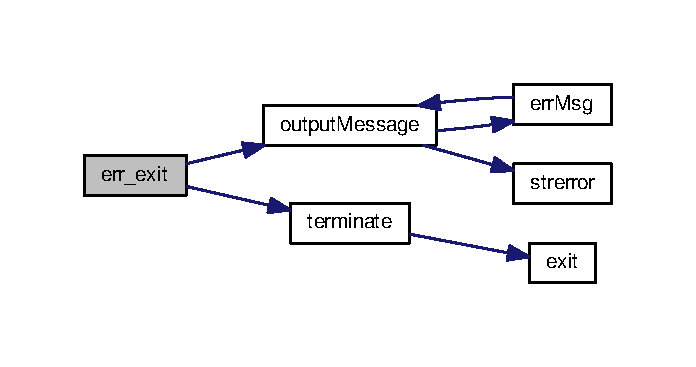
\includegraphics[width=334pt]{dd/d35/error__functions_8c_ad83bc66851be4582ec97ba670a95fa0a_cgraph}
\end{center}
\end{figure}


\hypertarget{error__functions_8c_a9353730adacb3417493e841dace8708b}{\index{error\-\_\-functions.\-c@{error\-\_\-functions.\-c}!err\-Exit@{err\-Exit}}
\index{err\-Exit@{err\-Exit}!error_functions.c@{error\-\_\-functions.\-c}}
\subsubsection[{err\-Exit}]{\setlength{\rightskip}{0pt plus 5cm}void err\-Exit (
\begin{DoxyParamCaption}
\item[{const char $\ast$}]{format, }
\item[{}]{...}
\end{DoxyParamCaption}
)}}\label{error__functions_8c_a9353730adacb3417493e841dace8708b}


\-: Method to print the message with errno message, with exit. 

\begin{DoxyAuthor}{Author}
\-: Ravi Prasad (India) 
\end{DoxyAuthor}


Definition at line 106 of file error\-\_\-functions.\-c.



Here is the call graph for this function\-:
\nopagebreak
\begin{figure}[H]
\begin{center}
\leavevmode
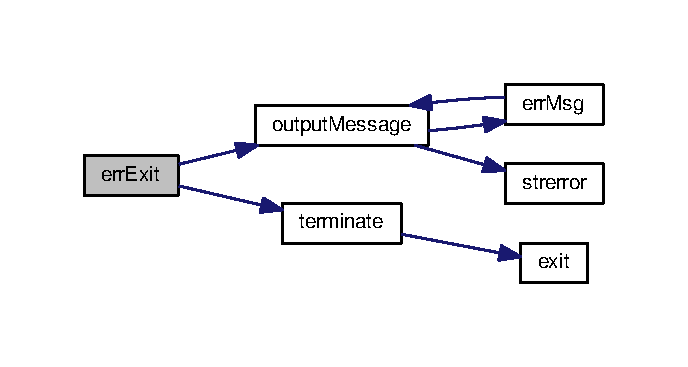
\includegraphics[width=330pt]{dd/d35/error__functions_8c_a9353730adacb3417493e841dace8708b_cgraph}
\end{center}
\end{figure}


\hypertarget{error__functions_8c_a88444cb888856a4241c156ae704e76de}{\index{error\-\_\-functions.\-c@{error\-\_\-functions.\-c}!err\-Exit\-E\-N@{err\-Exit\-E\-N}}
\index{err\-Exit\-E\-N@{err\-Exit\-E\-N}!error_functions.c@{error\-\_\-functions.\-c}}
\subsubsection[{err\-Exit\-E\-N}]{\setlength{\rightskip}{0pt plus 5cm}void err\-Exit\-E\-N (
\begin{DoxyParamCaption}
\item[{int}]{err\-Num, }
\item[{const char $\ast$}]{format, }
\item[{}]{...}
\end{DoxyParamCaption}
)}}\label{error__functions_8c_a88444cb888856a4241c156ae704e76de}


\-: Method to print the message with errno message, with exit call. 

\begin{DoxyAuthor}{Author}
\-: Ravi Prasad (India) 
\end{DoxyAuthor}


Definition at line 138 of file error\-\_\-functions.\-c.



Here is the call graph for this function\-:
\nopagebreak
\begin{figure}[H]
\begin{center}
\leavevmode
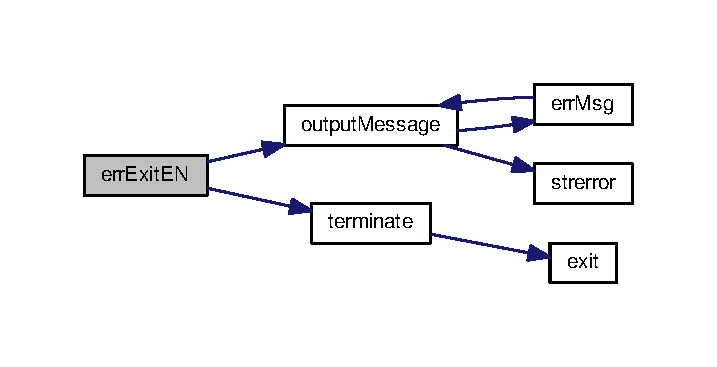
\includegraphics[width=344pt]{dd/d35/error__functions_8c_a88444cb888856a4241c156ae704e76de_cgraph}
\end{center}
\end{figure}


\hypertarget{error__functions_8c_a46c1ae408432a2c70da4402236454a5f}{\index{error\-\_\-functions.\-c@{error\-\_\-functions.\-c}!err\-Msg@{err\-Msg}}
\index{err\-Msg@{err\-Msg}!error_functions.c@{error\-\_\-functions.\-c}}
\subsubsection[{err\-Msg}]{\setlength{\rightskip}{0pt plus 5cm}void err\-Msg (
\begin{DoxyParamCaption}
\item[{const char $\ast$}]{format, }
\item[{}]{...}
\end{DoxyParamCaption}
)}}\label{error__functions_8c_a46c1ae408432a2c70da4402236454a5f}


\-: Method to print the message with errno message, without exit or \-\_\-exit call. 

\begin{DoxyAuthor}{Author}
\-: Ravi Prasad (India) 
\end{DoxyAuthor}


Definition at line 88 of file error\-\_\-functions.\-c.



Here is the call graph for this function\-:
\nopagebreak
\begin{figure}[H]
\begin{center}
\leavevmode
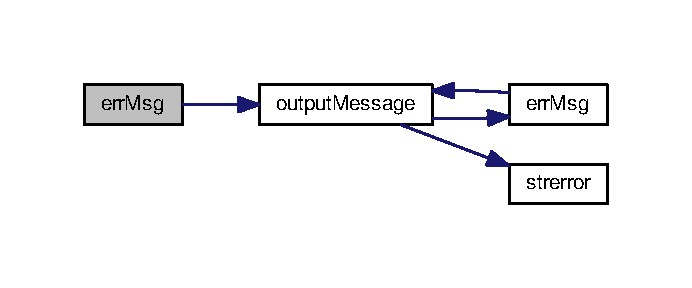
\includegraphics[width=332pt]{dd/d35/error__functions_8c_a46c1ae408432a2c70da4402236454a5f_cgraph}
\end{center}
\end{figure}




Here is the caller graph for this function\-:
\nopagebreak
\begin{figure}[H]
\begin{center}
\leavevmode
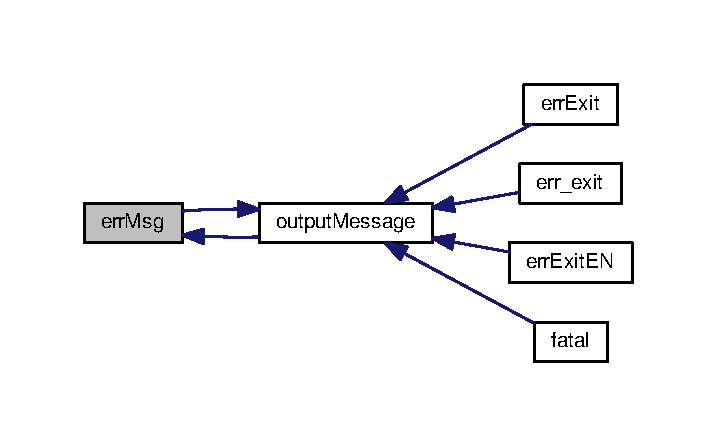
\includegraphics[width=344pt]{dd/d35/error__functions_8c_a46c1ae408432a2c70da4402236454a5f_icgraph}
\end{center}
\end{figure}


\hypertarget{error__functions_8c_abdee3dc73ec124f69d84a83af3ea90ce}{\index{error\-\_\-functions.\-c@{error\-\_\-functions.\-c}!fatal@{fatal}}
\index{fatal@{fatal}!error_functions.c@{error\-\_\-functions.\-c}}
\subsubsection[{fatal}]{\setlength{\rightskip}{0pt plus 5cm}void fatal (
\begin{DoxyParamCaption}
\item[{const char $\ast$}]{format, }
\item[{}]{...}
\end{DoxyParamCaption}
)}}\label{error__functions_8c_abdee3dc73ec124f69d84a83af3ea90ce}


\-: Method to print the message with errno message, with \-\_\-exit call. 

\begin{DoxyAuthor}{Author}
\-: Ravi Prasad (India) 
\end{DoxyAuthor}


Definition at line 154 of file error\-\_\-functions.\-c.



Here is the call graph for this function\-:
\nopagebreak
\begin{figure}[H]
\begin{center}
\leavevmode
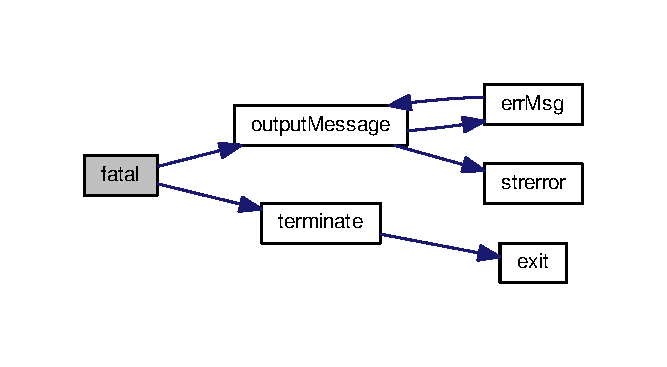
\includegraphics[width=320pt]{dd/d35/error__functions_8c_abdee3dc73ec124f69d84a83af3ea90ce_cgraph}
\end{center}
\end{figure}


\hypertarget{error__functions_8c_accffbc65d0a3df9ae8a527062ffddd05}{\index{error\-\_\-functions.\-c@{error\-\_\-functions.\-c}!output\-Message@{output\-Message}}
\index{output\-Message@{output\-Message}!error_functions.c@{error\-\_\-functions.\-c}}
\subsubsection[{output\-Message}]{\setlength{\rightskip}{0pt plus 5cm}static void output\-Message (
\begin{DoxyParamCaption}
\item[{{\bf B\-O\-O\-L\-E\-A\-N}}]{use\-Err\-No, }
\item[{int}]{err, }
\item[{{\bf B\-O\-O\-L\-E\-A\-N}}]{flush\-Buffer, }
\item[{const char $\ast$}]{format, }
\item[{va\-\_\-list}]{arg\-List}
\end{DoxyParamCaption}
)\hspace{0.3cm}{\ttfamily [static]}}}\label{error__functions_8c_accffbc65d0a3df9ae8a527062ffddd05}


\-: Method to print the message with or without errorno message. 

\begin{DoxyAuthor}{Author}
\-: Ravi Prasad (India) 
\end{DoxyAuthor}


Definition at line 53 of file error\-\_\-functions.\-c.



Here is the call graph for this function\-:
\nopagebreak
\begin{figure}[H]
\begin{center}
\leavevmode
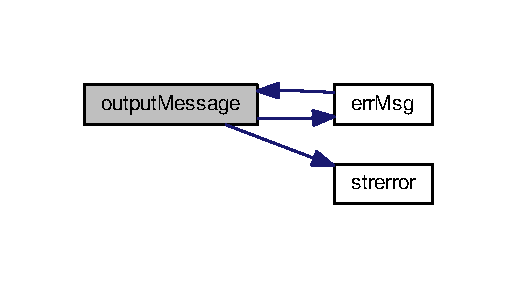
\includegraphics[width=248pt]{dd/d35/error__functions_8c_accffbc65d0a3df9ae8a527062ffddd05_cgraph}
\end{center}
\end{figure}




Here is the caller graph for this function\-:
\nopagebreak
\begin{figure}[H]
\begin{center}
\leavevmode
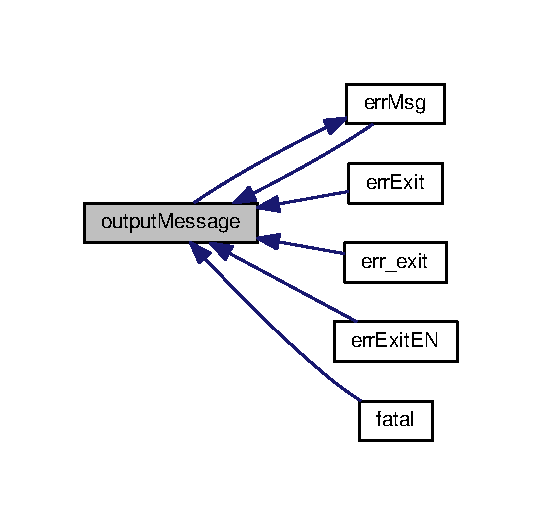
\includegraphics[width=260pt]{dd/d35/error__functions_8c_accffbc65d0a3df9ae8a527062ffddd05_icgraph}
\end{center}
\end{figure}


\hypertarget{error__functions_8c_ad0aaa18a5967e8ea284b980da0029f58}{\index{error\-\_\-functions.\-c@{error\-\_\-functions.\-c}!terminate@{terminate}}
\index{terminate@{terminate}!error_functions.c@{error\-\_\-functions.\-c}}
\subsubsection[{terminate}]{\setlength{\rightskip}{0pt plus 5cm}static void terminate (
\begin{DoxyParamCaption}
\item[{{\bf B\-O\-O\-L\-E\-A\-N}}]{use\-Exit}
\end{DoxyParamCaption}
)\hspace{0.3cm}{\ttfamily [static]}}}\label{error__functions_8c_ad0aaa18a5967e8ea284b980da0029f58}


\-: Note\-: Difference between \hyperlink{common_2README_a85c39bfe84eed5e1d7dae87fb0018669}{exit()} and \-\_\-exit() 

There are the differences\-: \-\_\-exit() won't flushes the stdio buffer while \hyperlink{common_2README_a85c39bfe84eed5e1d7dae87fb0018669}{exit()} flushes the stdio buffer prior to exit. \-\_\-exit() can not perform clean-\/up process while \hyperlink{common_2README_a85c39bfe84eed5e1d7dae87fb0018669}{exit()} can be registered with some function. ( i.\-e on\-\_\-exit or at\-\_\-exit) to perform some clean-\/up process if anything is required before existing the program.

exit(status) simply passes the exit status to \-\_\-exit(status). It is recommended that whenever to perform fork(), one of them between child and parent, one use \-\_\-exit() and another use \hyperlink{common_2README_a85c39bfe84eed5e1d7dae87fb0018669}{exit()}. \begin{DoxyAuthor}{Author}
\-: Ravi Prasad (India)
\end{DoxyAuthor}
\-: termination function with the provision of core dump \mbox{[}Y\-E\-S/\-N\-O\mbox{]} 

Definition at line 31 of file error\-\_\-functions.\-c.



Here is the call graph for this function\-:
\nopagebreak
\begin{figure}[H]
\begin{center}
\leavevmode
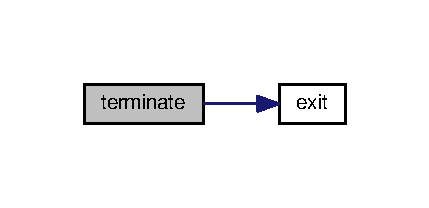
\includegraphics[width=206pt]{dd/d35/error__functions_8c_ad0aaa18a5967e8ea284b980da0029f58_cgraph}
\end{center}
\end{figure}




Here is the caller graph for this function\-:
\nopagebreak
\begin{figure}[H]
\begin{center}
\leavevmode
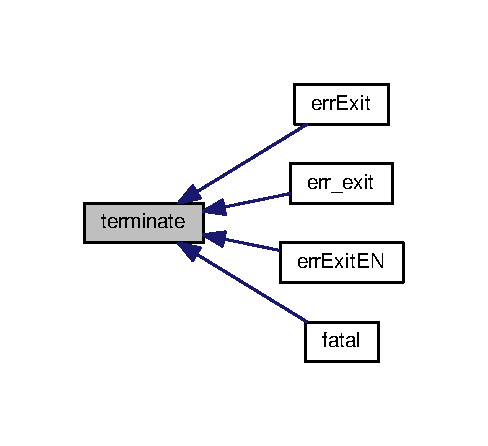
\includegraphics[width=234pt]{dd/d35/error__functions_8c_ad0aaa18a5967e8ea284b980da0029f58_icgraph}
\end{center}
\end{figure}


\hypertarget{error__functions_8c_a0c81140d074e6630634e05e7ca437390}{\index{error\-\_\-functions.\-c@{error\-\_\-functions.\-c}!usage\-Err@{usage\-Err}}
\index{usage\-Err@{usage\-Err}!error_functions.c@{error\-\_\-functions.\-c}}
\subsubsection[{usage\-Err}]{\setlength{\rightskip}{0pt plus 5cm}void usage\-Err (
\begin{DoxyParamCaption}
\item[{const char $\ast$}]{format, }
\item[{}]{...}
\end{DoxyParamCaption}
)}}\label{error__functions_8c_a0c81140d074e6630634e05e7ca437390}


\-: Method to print the uses error. 

\begin{DoxyAuthor}{Author}
\-: Ravi Prasad (India) 
\end{DoxyAuthor}


Definition at line 169 of file error\-\_\-functions.\-c.



Here is the call graph for this function\-:
\nopagebreak
\begin{figure}[H]
\begin{center}
\leavevmode
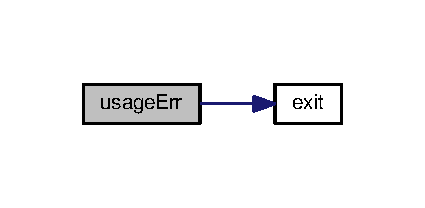
\includegraphics[width=204pt]{dd/d35/error__functions_8c_a0c81140d074e6630634e05e7ca437390_cgraph}
\end{center}
\end{figure}



\hypertarget{get__num_8c}{\section{common/source/get\-\_\-num.c File Reference}
\label{get__num_8c}\index{common/source/get\-\_\-num.\-c@{common/source/get\-\_\-num.\-c}}
}
{\ttfamily \#include $<$get\-\_\-num.\-h$>$}\\*
{\ttfamily \#include \char`\"{}tlpi\-\_\-hdr.\-h\char`\"{}}\\*
Include dependency graph for get\-\_\-num.\-c\-:
\nopagebreak
\begin{figure}[H]
\begin{center}
\leavevmode
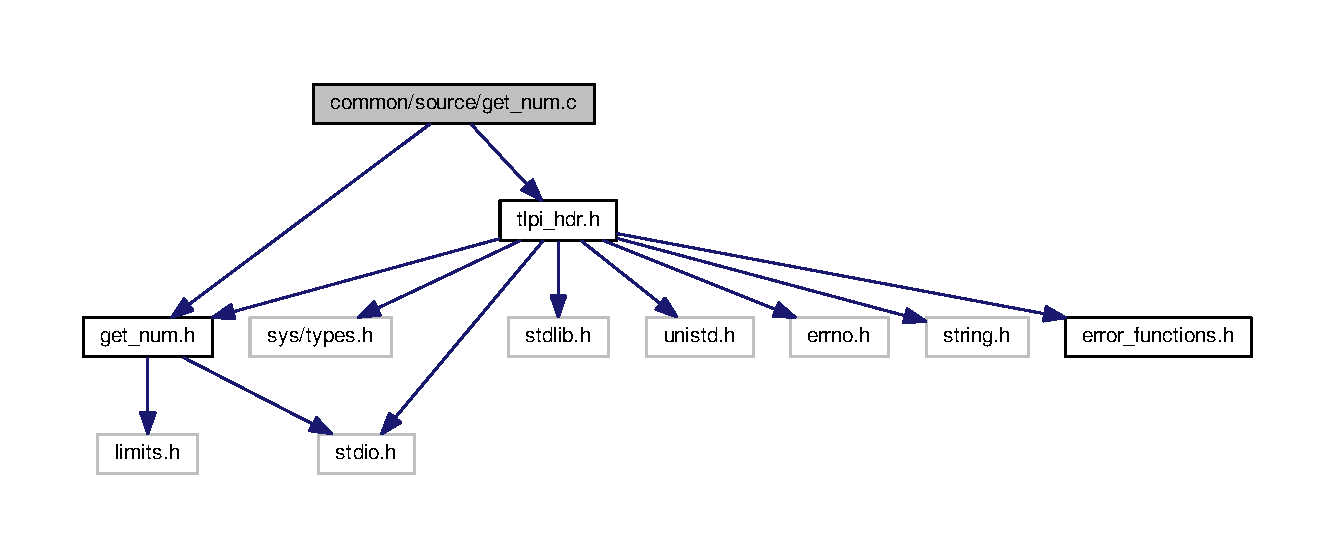
\includegraphics[width=350pt]{d8/dae/get__num_8c__incl}
\end{center}
\end{figure}
\subsection*{Functions}
\begin{DoxyCompactItemize}
\item 
\hyperlink{tlpi__hdr_8h_aec7e62084419d7857ae740a4c68241cf}{B\-O\-O\-L\-E\-A\-N} \hyperlink{get__num_8c_a86a1da723ab14c99d2b85920f888bb5c}{is\-Numeric\-Char} (char x)
\item 
int \hyperlink{get__num_8c_aafea1112c7333dcfa49a8d051c2bde9a}{my\-Atoi} (char $\ast$str)
\item 
long \hyperlink{get__num_8c_afc17dbeb125e1388078e1a9221624f15}{my\-Atol} (char $\ast$str)
\end{DoxyCompactItemize}


\subsection{Function Documentation}
\hypertarget{get__num_8c_a86a1da723ab14c99d2b85920f888bb5c}{\index{get\-\_\-num.\-c@{get\-\_\-num.\-c}!is\-Numeric\-Char@{is\-Numeric\-Char}}
\index{is\-Numeric\-Char@{is\-Numeric\-Char}!get_num.c@{get\-\_\-num.\-c}}
\subsubsection[{is\-Numeric\-Char}]{\setlength{\rightskip}{0pt plus 5cm}{\bf B\-O\-O\-L\-E\-A\-N} is\-Numeric\-Char (
\begin{DoxyParamCaption}
\item[{char}]{x}
\end{DoxyParamCaption}
)}}\label{get__num_8c_a86a1da723ab14c99d2b85920f888bb5c}


Definition at line 5 of file get\-\_\-num.\-c.



Here is the caller graph for this function\-:
\nopagebreak
\begin{figure}[H]
\begin{center}
\leavevmode
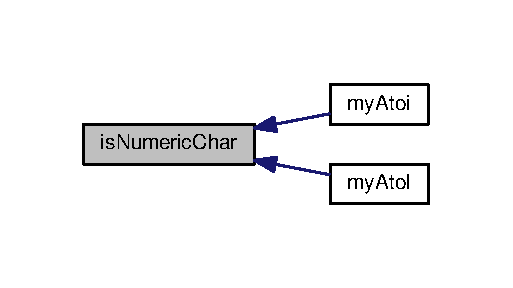
\includegraphics[width=246pt]{d6/dcd/get__num_8c_a86a1da723ab14c99d2b85920f888bb5c_icgraph}
\end{center}
\end{figure}


\hypertarget{get__num_8c_aafea1112c7333dcfa49a8d051c2bde9a}{\index{get\-\_\-num.\-c@{get\-\_\-num.\-c}!my\-Atoi@{my\-Atoi}}
\index{my\-Atoi@{my\-Atoi}!get_num.c@{get\-\_\-num.\-c}}
\subsubsection[{my\-Atoi}]{\setlength{\rightskip}{0pt plus 5cm}int my\-Atoi (
\begin{DoxyParamCaption}
\item[{char $\ast$}]{str}
\end{DoxyParamCaption}
)}}\label{get__num_8c_aafea1112c7333dcfa49a8d051c2bde9a}
cutomize atoi 

Definition at line 12 of file get\-\_\-num.\-c.



Here is the call graph for this function\-:
\nopagebreak
\begin{figure}[H]
\begin{center}
\leavevmode
\includegraphics[width=246pt]{d6/dcd/get__num_8c_aafea1112c7333dcfa49a8d051c2bde9a_cgraph}
\end{center}
\end{figure}


\hypertarget{get__num_8c_afc17dbeb125e1388078e1a9221624f15}{\index{get\-\_\-num.\-c@{get\-\_\-num.\-c}!my\-Atol@{my\-Atol}}
\index{my\-Atol@{my\-Atol}!get_num.c@{get\-\_\-num.\-c}}
\subsubsection[{my\-Atol}]{\setlength{\rightskip}{0pt plus 5cm}long my\-Atol (
\begin{DoxyParamCaption}
\item[{char $\ast$}]{str}
\end{DoxyParamCaption}
)}}\label{get__num_8c_afc17dbeb125e1388078e1a9221624f15}


Definition at line 44 of file get\-\_\-num.\-c.



Here is the call graph for this function\-:
\nopagebreak
\begin{figure}[H]
\begin{center}
\leavevmode
\includegraphics[width=246pt]{d6/dcd/get__num_8c_afc17dbeb125e1388078e1a9221624f15_cgraph}
\end{center}
\end{figure}



\hypertarget{aupe_8h}{\section{logging/include/aupe.h File Reference}
\label{aupe_8h}\index{logging/include/aupe.\-h@{logging/include/aupe.\-h}}
}
{\ttfamily \#include $<$stdio.\-h$>$}\\*
{\ttfamily \#include $<$fcntl.\-h$>$}\\*
{\ttfamily \#include $<$unistd.\-h$>$}\\*
{\ttfamily \#include $<$stdlib.\-h$>$}\\*
{\ttfamily \#include $<$errno.\-h$>$}\\*
{\ttfamily \#include $<$sys/types.\-h$>$}\\*
{\ttfamily \#include $<$sys/stat.\-h$>$}\\*
{\ttfamily \#include $<$sys/ioctl.\-h$>$}\\*
{\ttfamily \#include $<$sys/wait.\-h$>$}\\*
{\ttfamily \#include $<$string.\-h$>$}\\*
{\ttfamily \#include $<$malloc.\-h$>$}\\*
{\ttfamily \#include $<$iostream$>$}\\*
{\ttfamily \#include $<$string$>$}\\*
{\ttfamily \#include $<$fstream$>$}\\*
{\ttfamily \#include $<$cstring$>$}\\*
{\ttfamily \#include $<$cstdarg$>$}\\*
{\ttfamily \#include $<$iomanip$>$}\\*
Include dependency graph for aupe.\-h\-:
\nopagebreak
\begin{figure}[H]
\begin{center}
\leavevmode
\includegraphics[width=350pt]{d2/dea/aupe_8h__incl}
\end{center}
\end{figure}
This graph shows which files directly or indirectly include this file\-:
\nopagebreak
\begin{figure}[H]
\begin{center}
\leavevmode
\includegraphics[width=350pt]{de/dc4/aupe_8h__dep__incl}
\end{center}
\end{figure}
\subsection*{Macros}
\begin{DoxyCompactItemize}
\item 
\#define \hyperlink{aupe_8h_ae5e23dea252ef3137f9d0e5e63b0d770}{oflag}~O\-\_\-\-C\-R\-E\-A\-T$|$O\-\_\-\-R\-D\-W\-R$|$O\-\_\-\-T\-R\-U\-N\-C
\item 
\#define \hyperlink{aupe_8h_af613cadd5cf49515a2b8790d3bfd56af}{mode}~0666
\end{DoxyCompactItemize}


\subsection{Macro Definition Documentation}
\hypertarget{aupe_8h_af613cadd5cf49515a2b8790d3bfd56af}{\index{aupe.\-h@{aupe.\-h}!mode@{mode}}
\index{mode@{mode}!aupe.h@{aupe.\-h}}
\subsubsection[{mode}]{\setlength{\rightskip}{0pt plus 5cm}\#define mode~0666}}\label{aupe_8h_af613cadd5cf49515a2b8790d3bfd56af}


Definition at line 26 of file aupe.\-h.

\hypertarget{aupe_8h_ae5e23dea252ef3137f9d0e5e63b0d770}{\index{aupe.\-h@{aupe.\-h}!oflag@{oflag}}
\index{oflag@{oflag}!aupe.h@{aupe.\-h}}
\subsubsection[{oflag}]{\setlength{\rightskip}{0pt plus 5cm}\#define oflag~O\-\_\-\-C\-R\-E\-A\-T$|$O\-\_\-\-R\-D\-W\-R$|$O\-\_\-\-T\-R\-U\-N\-C}}\label{aupe_8h_ae5e23dea252ef3137f9d0e5e63b0d770}


Definition at line 25 of file aupe.\-h.


\hypertarget{CLogger_8h}{\section{logging/include/\-C\-Logger.h File Reference}
\label{CLogger_8h}\index{logging/include/\-C\-Logger.\-h@{logging/include/\-C\-Logger.\-h}}
}
{\ttfamily \#include \char`\"{}aupe.\-h\char`\"{}}\\*
Include dependency graph for C\-Logger.\-h\-:
\nopagebreak
\begin{figure}[H]
\begin{center}
\leavevmode
\includegraphics[width=350pt]{df/db9/CLogger_8h__incl}
\end{center}
\end{figure}
This graph shows which files directly or indirectly include this file\-:
\nopagebreak
\begin{figure}[H]
\begin{center}
\leavevmode
\includegraphics[width=350pt]{d2/df0/CLogger_8h__dep__incl}
\end{center}
\end{figure}
\subsection*{Classes}
\begin{DoxyCompactItemize}
\item 
class \hyperlink{classCLogger}{C\-Logger}
\begin{DoxyCompactList}\small\item\em \-: It is a singleton Logger class Can we use in multithreading This class is used for logging the erro, warning or information. T\-O Do\-: Need to leverage for verbositiy level. \end{DoxyCompactList}\end{DoxyCompactItemize}
\subsection*{Macros}
\begin{DoxyCompactItemize}
\item 
\#define \hyperlink{CLogger_8h_aa385268d3ec7b4d3ecceb7c787171bf0}{L\-O\-G\-G\-E\-R}~\hyperlink{classCLogger_a9b863cc897927485856833316b2dcffc}{C\-Logger\-::\-Get\-Logger}()
\end{DoxyCompactItemize}


\subsection{Macro Definition Documentation}
\hypertarget{CLogger_8h_aa385268d3ec7b4d3ecceb7c787171bf0}{\index{C\-Logger.\-h@{C\-Logger.\-h}!L\-O\-G\-G\-E\-R@{L\-O\-G\-G\-E\-R}}
\index{L\-O\-G\-G\-E\-R@{L\-O\-G\-G\-E\-R}!CLogger.h@{C\-Logger.\-h}}
\subsubsection[{L\-O\-G\-G\-E\-R}]{\setlength{\rightskip}{0pt plus 5cm}\#define L\-O\-G\-G\-E\-R~{\bf C\-Logger\-::\-Get\-Logger}()}}\label{CLogger_8h_aa385268d3ec7b4d3ecceb7c787171bf0}


Definition at line 4 of file C\-Logger.\-h.


\hypertarget{CLoggerException_8h}{\section{logging/include/\-C\-Logger\-Exception.h File Reference}
\label{CLoggerException_8h}\index{logging/include/\-C\-Logger\-Exception.\-h@{logging/include/\-C\-Logger\-Exception.\-h}}
}
{\ttfamily \#include \char`\"{}aupe.\-h\char`\"{}}\\*
Include dependency graph for C\-Logger\-Exception.\-h\-:
\nopagebreak
\begin{figure}[H]
\begin{center}
\leavevmode
\includegraphics[width=350pt]{d8/d2b/CLoggerException_8h__incl}
\end{center}
\end{figure}
This graph shows which files directly or indirectly include this file\-:
\nopagebreak
\begin{figure}[H]
\begin{center}
\leavevmode
\includegraphics[width=262pt]{d3/d97/CLoggerException_8h__dep__incl}
\end{center}
\end{figure}
\subsection*{Classes}
\begin{DoxyCompactItemize}
\item 
class \hyperlink{classCLoggerException}{C\-Logger\-Exception}
\end{DoxyCompactItemize}

\hypertarget{CMutex_8h}{\section{logging/include/\-C\-Mutex.h File Reference}
\label{CMutex_8h}\index{logging/include/\-C\-Mutex.\-h@{logging/include/\-C\-Mutex.\-h}}
}
{\ttfamily \#include $<$pthread.\-h$>$}\\*
Include dependency graph for C\-Mutex.\-h\-:
\nopagebreak
\begin{figure}[H]
\begin{center}
\leavevmode
\includegraphics[width=206pt]{df/da4/CMutex_8h__incl}
\end{center}
\end{figure}
This graph shows which files directly or indirectly include this file\-:
\nopagebreak
\begin{figure}[H]
\begin{center}
\leavevmode
\includegraphics[width=218pt]{dc/d79/CMutex_8h__dep__incl}
\end{center}
\end{figure}
\subsection*{Classes}
\begin{DoxyCompactItemize}
\item 
class \hyperlink{classCMutex}{C\-Mutex}
\begin{DoxyCompactList}\small\item\em \-: Mutex class to achieve synchronization \end{DoxyCompactList}\end{DoxyCompactItemize}

\hypertarget{DateTiime_8h}{\section{logging/include/\-Date\-Tiime.h File Reference}
\label{DateTiime_8h}\index{logging/include/\-Date\-Tiime.\-h@{logging/include/\-Date\-Tiime.\-h}}
}
{\ttfamily \#include $<$time.\-h$>$}\\*
{\ttfamily \#include \char`\"{}aupe.\-h\char`\"{}}\\*
Include dependency graph for Date\-Tiime.\-h\-:
\nopagebreak
\begin{figure}[H]
\begin{center}
\leavevmode
\includegraphics[width=350pt]{da/d19/DateTiime_8h__incl}
\end{center}
\end{figure}
This graph shows which files directly or indirectly include this file\-:
\nopagebreak
\begin{figure}[H]
\begin{center}
\leavevmode
\includegraphics[width=218pt]{d6/d63/DateTiime_8h__dep__incl}
\end{center}
\end{figure}
\subsection*{Namespaces}
\begin{DoxyCompactItemize}
\item 
\hyperlink{namespaceDateTime}{Date\-Time}
\end{DoxyCompactItemize}
\subsection*{Functions}
\begin{DoxyCompactItemize}
\item 
const std\-::string \hyperlink{namespaceDateTime_a7d1e8972f688ff552761398f0f75293b}{Date\-Time\-::get\-Current\-Date\-Time} ()
\end{DoxyCompactItemize}

\hypertarget{CLogger_8cpp}{\section{logging/source/\-C\-Logger.cpp File Reference}
\label{CLogger_8cpp}\index{logging/source/\-C\-Logger.\-cpp@{logging/source/\-C\-Logger.\-cpp}}
}
{\ttfamily \#include \char`\"{}C\-Logger.\-h\char`\"{}}\\*
{\ttfamily \#include \char`\"{}Date\-Tiime.\-h\char`\"{}}\\*
{\ttfamily \#include \char`\"{}C\-Mutex.\-h\char`\"{}}\\*
Include dependency graph for C\-Logger.\-cpp\-:
\nopagebreak
\begin{figure}[H]
\begin{center}
\leavevmode
\includegraphics[width=350pt]{d0/d82/CLogger_8cpp__incl}
\end{center}
\end{figure}

\hypertarget{CLoggerException_8cpp}{\section{logging/source/\-C\-Logger\-Exception.cpp File Reference}
\label{CLoggerException_8cpp}\index{logging/source/\-C\-Logger\-Exception.\-cpp@{logging/source/\-C\-Logger\-Exception.\-cpp}}
}
{\ttfamily \#include \char`\"{}C\-Logger\-Exception.\-h\char`\"{}}\\*
Include dependency graph for C\-Logger\-Exception.\-cpp\-:
\nopagebreak
\begin{figure}[H]
\begin{center}
\leavevmode
\includegraphics[width=350pt]{d5/ddb/CLoggerException_8cpp__incl}
\end{center}
\end{figure}

\hypertarget{inet__accept_8h}{\section{tcp\-Socket/include/inet\-\_\-accept.h File Reference}
\label{inet__accept_8h}\index{tcp\-Socket/include/inet\-\_\-accept.\-h@{tcp\-Socket/include/inet\-\_\-accept.\-h}}
}
This graph shows which files directly or indirectly include this file\-:
\nopagebreak
\begin{figure}[H]
\begin{center}
\leavevmode
\includegraphics[width=311pt]{d9/d55/inet__accept_8h__dep__incl}
\end{center}
\end{figure}
\subsection*{Macros}
\begin{DoxyCompactItemize}
\item 
\#define \hyperlink{inet__accept_8h_aa8cecfc5c5c054d2875c03e77b7be15d}{T\-R\-U\-E}~1
\item 
\#define \hyperlink{inet__accept_8h_aa93f0eb578d23995850d61f7d61c55c1}{F\-A\-L\-S\-E}~0
\end{DoxyCompactItemize}
\subsection*{Functions}
\begin{DoxyCompactItemize}
\item 
int \hyperlink{inet__accept_8h_ad7ca1270d91921eb3b2502d3bc6fec19}{non\-\_\-blocking\-\_\-accept} (const int listen\-\_\-sd)
\item 
int \hyperlink{inet__accept_8h_a536ce6b1ae81f3a65fbeba3b83226f91}{blocking\-\_\-accept} (const int listen\-\_\-sd)
\end{DoxyCompactItemize}


\subsection{Macro Definition Documentation}
\hypertarget{inet__accept_8h_aa93f0eb578d23995850d61f7d61c55c1}{\index{inet\-\_\-accept.\-h@{inet\-\_\-accept.\-h}!F\-A\-L\-S\-E@{F\-A\-L\-S\-E}}
\index{F\-A\-L\-S\-E@{F\-A\-L\-S\-E}!inet_accept.h@{inet\-\_\-accept.\-h}}
\subsubsection[{F\-A\-L\-S\-E}]{\setlength{\rightskip}{0pt plus 5cm}\#define F\-A\-L\-S\-E~0}}\label{inet__accept_8h_aa93f0eb578d23995850d61f7d61c55c1}


Definition at line 5 of file inet\-\_\-accept.\-h.

\hypertarget{inet__accept_8h_aa8cecfc5c5c054d2875c03e77b7be15d}{\index{inet\-\_\-accept.\-h@{inet\-\_\-accept.\-h}!T\-R\-U\-E@{T\-R\-U\-E}}
\index{T\-R\-U\-E@{T\-R\-U\-E}!inet_accept.h@{inet\-\_\-accept.\-h}}
\subsubsection[{T\-R\-U\-E}]{\setlength{\rightskip}{0pt plus 5cm}\#define T\-R\-U\-E~1}}\label{inet__accept_8h_aa8cecfc5c5c054d2875c03e77b7be15d}


Definition at line 4 of file inet\-\_\-accept.\-h.



\subsection{Function Documentation}
\hypertarget{inet__accept_8h_a536ce6b1ae81f3a65fbeba3b83226f91}{\index{inet\-\_\-accept.\-h@{inet\-\_\-accept.\-h}!blocking\-\_\-accept@{blocking\-\_\-accept}}
\index{blocking\-\_\-accept@{blocking\-\_\-accept}!inet_accept.h@{inet\-\_\-accept.\-h}}
\subsubsection[{blocking\-\_\-accept}]{\setlength{\rightskip}{0pt plus 5cm}int blocking\-\_\-accept (
\begin{DoxyParamCaption}
\item[{const int}]{listen\-\_\-sd}
\end{DoxyParamCaption}
)}}\label{inet__accept_8h_a536ce6b1ae81f3a65fbeba3b83226f91}
\hypertarget{inet__accept_8h_ad7ca1270d91921eb3b2502d3bc6fec19}{\index{inet\-\_\-accept.\-h@{inet\-\_\-accept.\-h}!non\-\_\-blocking\-\_\-accept@{non\-\_\-blocking\-\_\-accept}}
\index{non\-\_\-blocking\-\_\-accept@{non\-\_\-blocking\-\_\-accept}!inet_accept.h@{inet\-\_\-accept.\-h}}
\subsubsection[{non\-\_\-blocking\-\_\-accept}]{\setlength{\rightskip}{0pt plus 5cm}int non\-\_\-blocking\-\_\-accept (
\begin{DoxyParamCaption}
\item[{const int}]{listen\-\_\-sd}
\end{DoxyParamCaption}
)}}\label{inet__accept_8h_ad7ca1270d91921eb3b2502d3bc6fec19}
\begin{DoxyAuthor}{Author}
\-:Ravi Prasad (India)
\end{DoxyAuthor}
\-:The method accept multiple new connections and also response back the existing connection I/\-O. 
\begin{DoxyParams}{Parameters}
{\em \-:} & \mbox{[}I\-N\mbox{]} listen\-\_\-fd \{The fd return with the socket() \} \\
\hline
\end{DoxyParams}
\begin{DoxyReturn}{Returns}
\-: status -\/1 for fail 0 for success. 
\end{DoxyReturn}


Definition at line 22 of file inet\-\_\-accept.\-cpp.



Here is the call graph for this function\-:
\nopagebreak
\begin{figure}[H]
\begin{center}
\leavevmode
\includegraphics[width=326pt]{da/d4e/inet__accept_8h_ad7ca1270d91921eb3b2502d3bc6fec19_cgraph}
\end{center}
\end{figure}




Here is the caller graph for this function\-:
\nopagebreak
\begin{figure}[H]
\begin{center}
\leavevmode
\includegraphics[width=262pt]{da/d4e/inet__accept_8h_ad7ca1270d91921eb3b2502d3bc6fec19_icgraph}
\end{center}
\end{figure}



\hypertarget{include_2inet__handle__multiplex__io_8cpp}{\section{tcp\-Socket/include/inet\-\_\-handle\-\_\-multiplex\-\_\-io.cpp File Reference}
\label{include_2inet__handle__multiplex__io_8cpp}\index{tcp\-Socket/include/inet\-\_\-handle\-\_\-multiplex\-\_\-io.\-cpp@{tcp\-Socket/include/inet\-\_\-handle\-\_\-multiplex\-\_\-io.\-cpp}}
}

\hypertarget{source_2inet__handle__multiplex__io_8cpp}{\section{tcp\-Socket/source/inet\-\_\-handle\-\_\-multiplex\-\_\-io.cpp File Reference}
\label{source_2inet__handle__multiplex__io_8cpp}\index{tcp\-Socket/source/inet\-\_\-handle\-\_\-multiplex\-\_\-io.\-cpp@{tcp\-Socket/source/inet\-\_\-handle\-\_\-multiplex\-\_\-io.\-cpp}}
}
{\ttfamily \#include $<$stdio.\-h$>$}\\*
{\ttfamily \#include $<$stdlib.\-h$>$}\\*
{\ttfamily \#include $<$string.\-h$>$}\\*
{\ttfamily \#include $<$unistd.\-h$>$}\\*
{\ttfamily \#include \char`\"{}inet\-\_\-socket.\-h\char`\"{}}\\*
{\ttfamily \#include \char`\"{}inet\-\_\-handle\-\_\-multiplex\-\_\-io.\-h\char`\"{}}\\*
{\ttfamily \#include \char`\"{}C\-Logger.\-h\char`\"{}}\\*
Include dependency graph for inet\-\_\-handle\-\_\-multiplex\-\_\-io.\-cpp\-:
\nopagebreak
\begin{figure}[H]
\begin{center}
\leavevmode
\includegraphics[width=350pt]{d4/dee/source_2inet__handle__multiplex__io_8cpp__incl}
\end{center}
\end{figure}
\subsection*{Macros}
\begin{DoxyCompactItemize}
\item 
\#define \hyperlink{source_2inet__handle__multiplex__io_8cpp_a16c16f9369be4a374a3e621f6d13bb16}{M\-A\-X\-D\-A\-T\-A\-S\-I\-Z\-E}~128
\end{DoxyCompactItemize}
\subsection*{Functions}
\begin{DoxyCompactItemize}
\item 
int \hyperlink{source_2inet__handle__multiplex__io_8cpp_a5b7d00b9255711bb21248a110db46c9a}{inet\-\_\-handle\-\_\-multiplex\-\_\-io} (const int sockfd, int nsec)
\begin{DoxyCompactList}\small\item\em \-: This method handles the non blocking I/\-O operation, can be use by both active and passive(client or server) socket to monitor multiple I/\-O at their side. uses select call for monitoring multiple I/\-Os. \end{DoxyCompactList}\end{DoxyCompactItemize}


\subsection{Macro Definition Documentation}
\hypertarget{source_2inet__handle__multiplex__io_8cpp_a16c16f9369be4a374a3e621f6d13bb16}{\index{source/inet\-\_\-handle\-\_\-multiplex\-\_\-io.\-cpp@{source/inet\-\_\-handle\-\_\-multiplex\-\_\-io.\-cpp}!M\-A\-X\-D\-A\-T\-A\-S\-I\-Z\-E@{M\-A\-X\-D\-A\-T\-A\-S\-I\-Z\-E}}
\index{M\-A\-X\-D\-A\-T\-A\-S\-I\-Z\-E@{M\-A\-X\-D\-A\-T\-A\-S\-I\-Z\-E}!source/inet_handle_multiplex_io.cpp@{source/inet\-\_\-handle\-\_\-multiplex\-\_\-io.\-cpp}}
\subsubsection[{M\-A\-X\-D\-A\-T\-A\-S\-I\-Z\-E}]{\setlength{\rightskip}{0pt plus 5cm}\#define M\-A\-X\-D\-A\-T\-A\-S\-I\-Z\-E~128}}\label{source_2inet__handle__multiplex__io_8cpp_a16c16f9369be4a374a3e621f6d13bb16}


Definition at line 9 of file inet\-\_\-handle\-\_\-multiplex\-\_\-io.\-cpp.



\subsection{Function Documentation}
\hypertarget{source_2inet__handle__multiplex__io_8cpp_a5b7d00b9255711bb21248a110db46c9a}{\index{source/inet\-\_\-handle\-\_\-multiplex\-\_\-io.\-cpp@{source/inet\-\_\-handle\-\_\-multiplex\-\_\-io.\-cpp}!inet\-\_\-handle\-\_\-multiplex\-\_\-io@{inet\-\_\-handle\-\_\-multiplex\-\_\-io}}
\index{inet\-\_\-handle\-\_\-multiplex\-\_\-io@{inet\-\_\-handle\-\_\-multiplex\-\_\-io}!source/inet_handle_multiplex_io.cpp@{source/inet\-\_\-handle\-\_\-multiplex\-\_\-io.\-cpp}}
\subsubsection[{inet\-\_\-handle\-\_\-multiplex\-\_\-io}]{\setlength{\rightskip}{0pt plus 5cm}int inet\-\_\-handle\-\_\-multiplex\-\_\-io (
\begin{DoxyParamCaption}
\item[{const int}]{sockfd, }
\item[{int}]{nsec}
\end{DoxyParamCaption}
)}}\label{source_2inet__handle__multiplex__io_8cpp_a5b7d00b9255711bb21248a110db46c9a}


\-: This method handles the non blocking I/\-O operation, can be use by both active and passive(client or server) socket to monitor multiple I/\-O at their side. uses select call for monitoring multiple I/\-Os. 

\begin{DoxyAuthor}{Author}
\-: Ravi Prasad (India).
\end{DoxyAuthor}

\begin{DoxyParams}{Parameters}
{\em \-:} & \mbox{[}in\mbox{]} sockfd \{socket/file fd monior for I/\-O\} \\
\hline
{\em \-:} & \mbox{[}in\mbox{]} nsec \{select timeout in seconds\} \\
\hline
\end{DoxyParams}


Definition at line 24 of file inet\-\_\-handle\-\_\-multiplex\-\_\-io.\-cpp.



Here is the caller graph for this function\-:
\nopagebreak
\begin{figure}[H]
\begin{center}
\leavevmode
\includegraphics[width=350pt]{d1/d52/source_2inet__handle__multiplex__io_8cpp_a5b7d00b9255711bb21248a110db46c9a_icgraph}
\end{center}
\end{figure}



\hypertarget{inet__handle__multiplex__io_8h}{\section{tcp\-Socket/include/inet\-\_\-handle\-\_\-multiplex\-\_\-io.h File Reference}
\label{inet__handle__multiplex__io_8h}\index{tcp\-Socket/include/inet\-\_\-handle\-\_\-multiplex\-\_\-io.\-h@{tcp\-Socket/include/inet\-\_\-handle\-\_\-multiplex\-\_\-io.\-h}}
}
This graph shows which files directly or indirectly include this file\-:
\nopagebreak
\begin{figure}[H]
\begin{center}
\leavevmode
\includegraphics[width=321pt]{de/d75/inet__handle__multiplex__io_8h__dep__incl}
\end{center}
\end{figure}
\subsection*{Functions}
\begin{DoxyCompactItemize}
\item 
int \hyperlink{inet__handle__multiplex__io_8h_a5b7d00b9255711bb21248a110db46c9a}{inet\-\_\-handle\-\_\-multiplex\-\_\-io} (const int sockfd, int nsec)
\begin{DoxyCompactList}\small\item\em \-: This method handles the non blocking I/\-O operation, can be use by both active and passive(client or server) socket to monitor multiple I/\-O at their side. uses select call for monitoring multiple I/\-Os. \end{DoxyCompactList}\end{DoxyCompactItemize}


\subsection{Function Documentation}
\hypertarget{inet__handle__multiplex__io_8h_a5b7d00b9255711bb21248a110db46c9a}{\index{inet\-\_\-handle\-\_\-multiplex\-\_\-io.\-h@{inet\-\_\-handle\-\_\-multiplex\-\_\-io.\-h}!inet\-\_\-handle\-\_\-multiplex\-\_\-io@{inet\-\_\-handle\-\_\-multiplex\-\_\-io}}
\index{inet\-\_\-handle\-\_\-multiplex\-\_\-io@{inet\-\_\-handle\-\_\-multiplex\-\_\-io}!inet_handle_multiplex_io.h@{inet\-\_\-handle\-\_\-multiplex\-\_\-io.\-h}}
\subsubsection[{inet\-\_\-handle\-\_\-multiplex\-\_\-io}]{\setlength{\rightskip}{0pt plus 5cm}int inet\-\_\-handle\-\_\-multiplex\-\_\-io (
\begin{DoxyParamCaption}
\item[{const int}]{sockfd, }
\item[{int}]{nsec}
\end{DoxyParamCaption}
)}}\label{inet__handle__multiplex__io_8h_a5b7d00b9255711bb21248a110db46c9a}


\-: This method handles the non blocking I/\-O operation, can be use by both active and passive(client or server) socket to monitor multiple I/\-O at their side. uses select call for monitoring multiple I/\-Os. 

\begin{DoxyAuthor}{Author}
\-: Ravi Prasad (India).
\end{DoxyAuthor}

\begin{DoxyParams}{Parameters}
{\em \-:} & \mbox{[}in\mbox{]} sockfd \{socket/file fd monior for I/\-O\} \\
\hline
{\em \-:} & \mbox{[}in\mbox{]} nsec \{select timeout in seconds\} \\
\hline
\end{DoxyParams}


Definition at line 24 of file inet\-\_\-handle\-\_\-multiplex\-\_\-io.\-cpp.



Here is the caller graph for this function\-:
\nopagebreak
\begin{figure}[H]
\begin{center}
\leavevmode
\includegraphics[width=350pt]{d4/d0c/inet__handle__multiplex__io_8h_a5b7d00b9255711bb21248a110db46c9a_icgraph}
\end{center}
\end{figure}



\hypertarget{inet__socket_8h}{\section{tcp\-Socket/include/inet\-\_\-socket.h File Reference}
\label{inet__socket_8h}\index{tcp\-Socket/include/inet\-\_\-socket.\-h@{tcp\-Socket/include/inet\-\_\-socket.\-h}}
}
{\ttfamily \#include \char`\"{}tcp\-\_\-common.\-h\char`\"{}}\\*
Include dependency graph for inet\-\_\-socket.\-h\-:
\nopagebreak
\begin{figure}[H]
\begin{center}
\leavevmode
\includegraphics[width=350pt]{dc/dda/inet__socket_8h__incl}
\end{center}
\end{figure}
This graph shows which files directly or indirectly include this file\-:
\nopagebreak
\begin{figure}[H]
\begin{center}
\leavevmode
\includegraphics[width=350pt]{d2/d52/inet__socket_8h__dep__incl}
\end{center}
\end{figure}
\subsection*{Macros}
\begin{DoxyCompactItemize}
\item 
\#define \hyperlink{inet__socket_8h_af1c5743a8f0c628d60a7a3ad85981765}{L\-I\-S\-T\-E\-N}~1
\item 
\#define \hyperlink{inet__socket_8h_aaa31440706ba11d449ccebfb07611495}{N\-O\-T\-\_\-\-L\-I\-S\-T\-E\-N}~0
\item 
\#define \hyperlink{inet__socket_8h_aeefbbafa97642defe3ee6c3080b7d66f}{B\-A\-C\-K\-L\-O\-G}~10
\item 
\#define \hyperlink{inet__socket_8h_a93d43db8a4edb54eec662981d4096fac}{P\-O\-R\-T\-\_\-\-N\-U\-M}~\char`\"{}50000\char`\"{}
\end{DoxyCompactItemize}
\subsection*{Functions}
\begin{DoxyCompactItemize}
\item 
void $\ast$ \hyperlink{inet__socket_8h_a294867ba9d7ff47e39d421134d8e12ab}{get\-\_\-in\-\_\-addr} (struct sockaddr $\ast$sa)
\begin{DoxyCompactList}\small\item\em \-: get sockaddr, I\-Pv4 or I\-Pv6 ip address Note\-: Used in inet\-\_\-ntop method. \end{DoxyCompactList}\item 
in\-\_\-port\-\_\-t \hyperlink{inet__socket_8h_a9cff4ecb4076bdcf7b759c9834d1f99b}{get\-\_\-in\-\_\-port} (struct sockaddr $\ast$sa)
\begin{DoxyCompactList}\small\item\em \-: get sockaddr, I\-Pv4 or I\-Pv6 port number Note\-: Used in ntohs method. \end{DoxyCompactList}\item 
int \hyperlink{inet__socket_8h_a88cba87b27a1dd999f206d996767578f}{get\-\_\-peer\-\_\-addr\-\_\-with\-\_\-peer\-\_\-sock} (const struct sockaddr $\ast$peer\-\_\-sock, char $\ast$peer\-\_\-name, unsigned short $\ast$port)
\begin{DoxyCompactList}\small\item\em \-: get sockaddr, I\-Pv4 or I\-Pv6 I\-P address and port number Note\-: Used to get the connecting client I\-P address and port number as a part of accept call. \end{DoxyCompactList}\item 
int \hyperlink{inet__socket_8h_a0d17436cdcdef6e93730b193008e9de8}{get\-\_\-peer\-\_\-addr\-\_\-with\-\_\-peer\-\_\-conn\-\_\-fd} (const int fd, char $\ast$peer\-\_\-name, unsigned short $\ast$port)
\begin{DoxyCompactList}\small\item\em \-: get sockaddr, I\-Pv4 or I\-Pv6 I\-P address and port number Note\-: Used to get the connecting client I\-P address and port number as a part of accept call. I prefer this call to get the detalis of peer or connecting client information. \end{DoxyCompactList}\item 
int \hyperlink{inet__socket_8h_ab37ff95ca876cde433bb18cca94956f2}{inet\-\_\-connect\-\_\-non\-\_\-blocking} (const char $\ast$host, const char $\ast$service, int socket\-\_\-type, int $\ast$connect\-\_\-fd)
\begin{DoxyCompactList}\small\item\em \-:Non Blocking connect call for the client. \end{DoxyCompactList}\item 
int \hyperlink{inet__socket_8h_a4ee3418bf7bd63c0b37ba13023d3e1cc}{inet\-\_\-connect\-\_\-blocking} (const char $\ast$host, const char $\ast$service, int socket\-\_\-type, int $\ast$connect\-\_\-fd)
\begin{DoxyCompactList}\small\item\em \-:Blocking connect call for the client. \end{DoxyCompactList}\item 
int \hyperlink{inet__socket_8h_a19ae7ff2c55d9c114a8effdcf9fae870}{inet\-\_\-passive} (const char $\ast$host, const char $\ast$service, int socket\-\_\-type, bool do\-\_\-listen, int backlog, int $\ast$listen\-\_\-fd, bool is\-\_\-non\-\_\-blocking=false)
\begin{DoxyCompactList}\small\item\em \-: Server side socket preparation method. It performs following tasks. \end{DoxyCompactList}\item 
int \hyperlink{inet__socket_8h_a3991cc2a47971acd778951add228bbc5}{inet\-\_\-bind} (const char $\ast$service, int sock\-\_\-type, int $\ast$listen\-\_\-fd, bool is\-\_\-non\-\_\-blocking)
\item 
int \hyperlink{inet__socket_8h_a9cde5897d9693cc6ad14bed0e118a656}{inet\-\_\-listen} (const char $\ast$host, const char $\ast$service, int sock\-\_\-type, int $\ast$listen\-\_\-fd, bool is\-\_\-non\-\_\-blocking)
\begin{DoxyCompactList}\small\item\em \-: This function creates a listening stream (S\-O\-C\-K\-\_\-\-S\-T\-R\-E\-A\-M) socket bound to the wildcard I\-P address on the T\-C\-P port specified by service. This function is designed for use by T\-C\-P servers \end{DoxyCompactList}\item 
bool \hyperlink{inet__socket_8h_ac77019092080908487c84b76e84d6cf9}{Set\-Socket\-Blocking\-Enabled} (const int fd, bool blocking)
\item 
int \hyperlink{inet__socket_8h_a3d36ce942d19fec8d8ca96c8218dac93}{inet\-\_\-non\-\_\-blocking\-\_\-connect} (int sockfd, const struct sockaddr $\ast$saptr, socklen\-\_\-t salen, int nsec)
\item 
int \hyperlink{inet__socket_8h_a2a1565c78d4308cc3178f652deb102a2}{inet\-\_\-non\-\_\-blocking\-\_\-accept} ()
\item 
bool \hyperlink{inet__socket_8h_a9f52927d084dddd6e0c6624a3a1ad909}{inet\-\_\-set\-\_\-socket\-\_\-non\-\_\-blocking} (const int fd, bool blocking)
\end{DoxyCompactItemize}


\subsection{Macro Definition Documentation}
\hypertarget{inet__socket_8h_aeefbbafa97642defe3ee6c3080b7d66f}{\index{inet\-\_\-socket.\-h@{inet\-\_\-socket.\-h}!B\-A\-C\-K\-L\-O\-G@{B\-A\-C\-K\-L\-O\-G}}
\index{B\-A\-C\-K\-L\-O\-G@{B\-A\-C\-K\-L\-O\-G}!inet_socket.h@{inet\-\_\-socket.\-h}}
\subsubsection[{B\-A\-C\-K\-L\-O\-G}]{\setlength{\rightskip}{0pt plus 5cm}\#define B\-A\-C\-K\-L\-O\-G~10}}\label{inet__socket_8h_aeefbbafa97642defe3ee6c3080b7d66f}


Definition at line 7 of file inet\-\_\-socket.\-h.

\hypertarget{inet__socket_8h_af1c5743a8f0c628d60a7a3ad85981765}{\index{inet\-\_\-socket.\-h@{inet\-\_\-socket.\-h}!L\-I\-S\-T\-E\-N@{L\-I\-S\-T\-E\-N}}
\index{L\-I\-S\-T\-E\-N@{L\-I\-S\-T\-E\-N}!inet_socket.h@{inet\-\_\-socket.\-h}}
\subsubsection[{L\-I\-S\-T\-E\-N}]{\setlength{\rightskip}{0pt plus 5cm}\#define L\-I\-S\-T\-E\-N~1}}\label{inet__socket_8h_af1c5743a8f0c628d60a7a3ad85981765}


Definition at line 5 of file inet\-\_\-socket.\-h.

\hypertarget{inet__socket_8h_aaa31440706ba11d449ccebfb07611495}{\index{inet\-\_\-socket.\-h@{inet\-\_\-socket.\-h}!N\-O\-T\-\_\-\-L\-I\-S\-T\-E\-N@{N\-O\-T\-\_\-\-L\-I\-S\-T\-E\-N}}
\index{N\-O\-T\-\_\-\-L\-I\-S\-T\-E\-N@{N\-O\-T\-\_\-\-L\-I\-S\-T\-E\-N}!inet_socket.h@{inet\-\_\-socket.\-h}}
\subsubsection[{N\-O\-T\-\_\-\-L\-I\-S\-T\-E\-N}]{\setlength{\rightskip}{0pt plus 5cm}\#define N\-O\-T\-\_\-\-L\-I\-S\-T\-E\-N~0}}\label{inet__socket_8h_aaa31440706ba11d449ccebfb07611495}


Definition at line 6 of file inet\-\_\-socket.\-h.

\hypertarget{inet__socket_8h_a93d43db8a4edb54eec662981d4096fac}{\index{inet\-\_\-socket.\-h@{inet\-\_\-socket.\-h}!P\-O\-R\-T\-\_\-\-N\-U\-M@{P\-O\-R\-T\-\_\-\-N\-U\-M}}
\index{P\-O\-R\-T\-\_\-\-N\-U\-M@{P\-O\-R\-T\-\_\-\-N\-U\-M}!inet_socket.h@{inet\-\_\-socket.\-h}}
\subsubsection[{P\-O\-R\-T\-\_\-\-N\-U\-M}]{\setlength{\rightskip}{0pt plus 5cm}\#define P\-O\-R\-T\-\_\-\-N\-U\-M~\char`\"{}50000\char`\"{}}}\label{inet__socket_8h_a93d43db8a4edb54eec662981d4096fac}


Definition at line 8 of file inet\-\_\-socket.\-h.



\subsection{Function Documentation}
\hypertarget{inet__socket_8h_a294867ba9d7ff47e39d421134d8e12ab}{\index{inet\-\_\-socket.\-h@{inet\-\_\-socket.\-h}!get\-\_\-in\-\_\-addr@{get\-\_\-in\-\_\-addr}}
\index{get\-\_\-in\-\_\-addr@{get\-\_\-in\-\_\-addr}!inet_socket.h@{inet\-\_\-socket.\-h}}
\subsubsection[{get\-\_\-in\-\_\-addr}]{\setlength{\rightskip}{0pt plus 5cm}void$\ast$ get\-\_\-in\-\_\-addr (
\begin{DoxyParamCaption}
\item[{struct sockaddr $\ast$}]{sa}
\end{DoxyParamCaption}
)}}\label{inet__socket_8h_a294867ba9d7ff47e39d421134d8e12ab}


\-: get sockaddr, I\-Pv4 or I\-Pv6 ip address Note\-: Used in inet\-\_\-ntop method. 

\begin{DoxyAuthor}{Author}
\-: Ravi Prasad (India)
\end{DoxyAuthor}

\begin{DoxyParams}{Parameters}
{\em \-:} & \mbox{[}in\mbox{]} sa sockaddr \\
\hline
\end{DoxyParams}
\begin{DoxyReturn}{Returns}
\-: struct sockaddr\-\_\-in/in6 with void 
\end{DoxyReturn}


Definition at line 15 of file inet\-\_\-socket.\-cpp.



Here is the caller graph for this function\-:
\nopagebreak
\begin{figure}[H]
\begin{center}
\leavevmode
\includegraphics[width=350pt]{d9/dc9/inet__socket_8h_a294867ba9d7ff47e39d421134d8e12ab_icgraph}
\end{center}
\end{figure}


\hypertarget{inet__socket_8h_a9cff4ecb4076bdcf7b759c9834d1f99b}{\index{inet\-\_\-socket.\-h@{inet\-\_\-socket.\-h}!get\-\_\-in\-\_\-port@{get\-\_\-in\-\_\-port}}
\index{get\-\_\-in\-\_\-port@{get\-\_\-in\-\_\-port}!inet_socket.h@{inet\-\_\-socket.\-h}}
\subsubsection[{get\-\_\-in\-\_\-port}]{\setlength{\rightskip}{0pt plus 5cm}in\-\_\-port\-\_\-t get\-\_\-in\-\_\-port (
\begin{DoxyParamCaption}
\item[{struct sockaddr $\ast$}]{sa}
\end{DoxyParamCaption}
)}}\label{inet__socket_8h_a9cff4ecb4076bdcf7b759c9834d1f99b}


\-: get sockaddr, I\-Pv4 or I\-Pv6 port number Note\-: Used in ntohs method. 

\begin{DoxyAuthor}{Author}
\-: Ravi Prasad (India)
\end{DoxyAuthor}

\begin{DoxyParams}{Parameters}
{\em \-:} & \mbox{[}in\mbox{]} sa sockaddr \\
\hline
\end{DoxyParams}
\begin{DoxyReturn}{Returns}
\-: struct sin/in6\-\_\-port 
\end{DoxyReturn}


Definition at line 36 of file inet\-\_\-socket.\-cpp.



Here is the caller graph for this function\-:
\nopagebreak
\begin{figure}[H]
\begin{center}
\leavevmode
\includegraphics[width=350pt]{d9/dc9/inet__socket_8h_a9cff4ecb4076bdcf7b759c9834d1f99b_icgraph}
\end{center}
\end{figure}


\hypertarget{inet__socket_8h_a0d17436cdcdef6e93730b193008e9de8}{\index{inet\-\_\-socket.\-h@{inet\-\_\-socket.\-h}!get\-\_\-peer\-\_\-addr\-\_\-with\-\_\-peer\-\_\-conn\-\_\-fd@{get\-\_\-peer\-\_\-addr\-\_\-with\-\_\-peer\-\_\-conn\-\_\-fd}}
\index{get\-\_\-peer\-\_\-addr\-\_\-with\-\_\-peer\-\_\-conn\-\_\-fd@{get\-\_\-peer\-\_\-addr\-\_\-with\-\_\-peer\-\_\-conn\-\_\-fd}!inet_socket.h@{inet\-\_\-socket.\-h}}
\subsubsection[{get\-\_\-peer\-\_\-addr\-\_\-with\-\_\-peer\-\_\-conn\-\_\-fd}]{\setlength{\rightskip}{0pt plus 5cm}int get\-\_\-peer\-\_\-addr\-\_\-with\-\_\-peer\-\_\-conn\-\_\-fd (
\begin{DoxyParamCaption}
\item[{const int}]{fd, }
\item[{char $\ast$}]{peer\-\_\-name, }
\item[{unsigned short $\ast$}]{peer\-\_\-port}
\end{DoxyParamCaption}
)}}\label{inet__socket_8h_a0d17436cdcdef6e93730b193008e9de8}


\-: get sockaddr, I\-Pv4 or I\-Pv6 I\-P address and port number Note\-: Used to get the connecting client I\-P address and port number as a part of accept call. I prefer this call to get the detalis of peer or connecting client information. 

\begin{DoxyAuthor}{Author}
\-: Ravi Prasad (India)
\end{DoxyAuthor}

\begin{DoxyParams}{Parameters}
{\em \-:} & \mbox{[}in\mbox{]} int fd \{accept api return value socket fd\} \\
\hline
{\em \-:} & \mbox{[}out\mbox{]} peer\-\_\-name \{connecting client name or I\-P\} \\
\hline
{\em \-:} & \mbox{[}out\mbox{]} peer\-\_\-port \{connecting client port number\} \\
\hline
\end{DoxyParams}
\begin{DoxyReturn}{Returns}
\-: -\/1 F\-A\-I\-L , 0 S\-U\-C\-C\-E\-S\-S 
\end{DoxyReturn}


Definition at line 104 of file inet\-\_\-socket.\-cpp.



Here is the caller graph for this function\-:
\nopagebreak
\begin{figure}[H]
\begin{center}
\leavevmode
\includegraphics[width=350pt]{d9/dc9/inet__socket_8h_a0d17436cdcdef6e93730b193008e9de8_icgraph}
\end{center}
\end{figure}


\hypertarget{inet__socket_8h_a88cba87b27a1dd999f206d996767578f}{\index{inet\-\_\-socket.\-h@{inet\-\_\-socket.\-h}!get\-\_\-peer\-\_\-addr\-\_\-with\-\_\-peer\-\_\-sock@{get\-\_\-peer\-\_\-addr\-\_\-with\-\_\-peer\-\_\-sock}}
\index{get\-\_\-peer\-\_\-addr\-\_\-with\-\_\-peer\-\_\-sock@{get\-\_\-peer\-\_\-addr\-\_\-with\-\_\-peer\-\_\-sock}!inet_socket.h@{inet\-\_\-socket.\-h}}
\subsubsection[{get\-\_\-peer\-\_\-addr\-\_\-with\-\_\-peer\-\_\-sock}]{\setlength{\rightskip}{0pt plus 5cm}int get\-\_\-peer\-\_\-addr\-\_\-with\-\_\-peer\-\_\-sock (
\begin{DoxyParamCaption}
\item[{const struct sockaddr $\ast$}]{peer\-\_\-sock, }
\item[{char $\ast$}]{peer\-\_\-name, }
\item[{unsigned short $\ast$}]{peer\-\_\-port}
\end{DoxyParamCaption}
)}}\label{inet__socket_8h_a88cba87b27a1dd999f206d996767578f}


\-: get sockaddr, I\-Pv4 or I\-Pv6 I\-P address and port number Note\-: Used to get the connecting client I\-P address and port number as a part of accept call. 

\begin{DoxyAuthor}{Author}
\-: Ravi Prasad (India)
\end{DoxyAuthor}

\begin{DoxyParams}{Parameters}
{\em \-:} & \mbox{[}in\mbox{]} sa sockaddr, accept api second parameter \\
\hline
{\em \-:} & \mbox{[}out\mbox{]} peer\-\_\-name \{connecting client name or I\-P\} \\
\hline
{\em \-:} & \mbox{[}out\mbox{]} peer\-\_\-port \{connecting client port number\} \\
\hline
\end{DoxyParams}
\begin{DoxyReturn}{Returns}
\-: -\/1 F\-A\-I\-L , 0 S\-U\-C\-C\-E\-S\-S 
\end{DoxyReturn}


Definition at line 62 of file inet\-\_\-socket.\-cpp.

\hypertarget{inet__socket_8h_a3991cc2a47971acd778951add228bbc5}{\index{inet\-\_\-socket.\-h@{inet\-\_\-socket.\-h}!inet\-\_\-bind@{inet\-\_\-bind}}
\index{inet\-\_\-bind@{inet\-\_\-bind}!inet_socket.h@{inet\-\_\-socket.\-h}}
\subsubsection[{inet\-\_\-bind}]{\setlength{\rightskip}{0pt plus 5cm}int inet\-\_\-bind (
\begin{DoxyParamCaption}
\item[{const char $\ast$}]{service, }
\item[{int}]{sock\-\_\-type, }
\item[{int $\ast$}]{listen\-\_\-fd, }
\item[{bool}]{is\-\_\-non\-\_\-blocking}
\end{DoxyParamCaption}
)}}\label{inet__socket_8h_a3991cc2a47971acd778951add228bbc5}
\hypertarget{inet__socket_8h_a4ee3418bf7bd63c0b37ba13023d3e1cc}{\index{inet\-\_\-socket.\-h@{inet\-\_\-socket.\-h}!inet\-\_\-connect\-\_\-blocking@{inet\-\_\-connect\-\_\-blocking}}
\index{inet\-\_\-connect\-\_\-blocking@{inet\-\_\-connect\-\_\-blocking}!inet_socket.h@{inet\-\_\-socket.\-h}}
\subsubsection[{inet\-\_\-connect\-\_\-blocking}]{\setlength{\rightskip}{0pt plus 5cm}int inet\-\_\-connect\-\_\-blocking (
\begin{DoxyParamCaption}
\item[{const char $\ast$}]{host, }
\item[{const char $\ast$}]{service, }
\item[{int}]{sock\-\_\-type, }
\item[{int $\ast$}]{connect\-\_\-fd}
\end{DoxyParamCaption}
)}}\label{inet__socket_8h_a4ee3418bf7bd63c0b37ba13023d3e1cc}


\-:Blocking connect call for the client. 

\begin{DoxyAuthor}{Author}
\-: Ravi Prasad (India)
\end{DoxyAuthor}

\begin{DoxyParams}{Parameters}
{\em \-:\mbox{[}in\mbox{]}} & host \{host name/url of the server.\} \\
\hline
{\em \-:\mbox{[}in\mbox{]}} & service \{port number or service name\} \\
\hline
{\em \-:\mbox{[}in\mbox{]}} & sock\-\_\-type \{type of socket S\-T\-R\-E\-A\-M/\-D\-G\-R\-A\-M\} \\
\hline
{\em \-:\mbox{[}out\mbox{]}} & connected fd \\
\hline
\end{DoxyParams}
\begin{DoxyReturn}{Returns}
\-:status -\/1\-: F\-A\-I\-L $>$0 \-: S\-U\-C\-C\-E\-S\-S. 
\end{DoxyReturn}


Definition at line 171 of file inet\-\_\-socket.\-cpp.



Here is the call graph for this function\-:
\nopagebreak
\begin{figure}[H]
\begin{center}
\leavevmode
\includegraphics[width=298pt]{d9/dc9/inet__socket_8h_a4ee3418bf7bd63c0b37ba13023d3e1cc_cgraph}
\end{center}
\end{figure}


\hypertarget{inet__socket_8h_ab37ff95ca876cde433bb18cca94956f2}{\index{inet\-\_\-socket.\-h@{inet\-\_\-socket.\-h}!inet\-\_\-connect\-\_\-non\-\_\-blocking@{inet\-\_\-connect\-\_\-non\-\_\-blocking}}
\index{inet\-\_\-connect\-\_\-non\-\_\-blocking@{inet\-\_\-connect\-\_\-non\-\_\-blocking}!inet_socket.h@{inet\-\_\-socket.\-h}}
\subsubsection[{inet\-\_\-connect\-\_\-non\-\_\-blocking}]{\setlength{\rightskip}{0pt plus 5cm}int inet\-\_\-connect\-\_\-non\-\_\-blocking (
\begin{DoxyParamCaption}
\item[{const char $\ast$}]{host, }
\item[{const char $\ast$}]{service, }
\item[{int}]{sock\-\_\-type, }
\item[{int $\ast$}]{connect\-\_\-fd}
\end{DoxyParamCaption}
)}}\label{inet__socket_8h_ab37ff95ca876cde433bb18cca94956f2}


\-:Non Blocking connect call for the client. 

\begin{DoxyAuthor}{Author}
\-: Ravi Prasad (India)
\end{DoxyAuthor}

\begin{DoxyParams}{Parameters}
{\em \-:\mbox{[}in\mbox{]}} & host \{host name/url of the server.\} \\
\hline
{\em \-:\mbox{[}in\mbox{]}} & service \{port number or service name\} \\
\hline
{\em \-:\mbox{[}in\mbox{]}} & sock\-\_\-type \{type of socket S\-T\-R\-E\-A\-M/\-D\-G\-R\-A\-M\} \\
\hline
{\em \-:\mbox{[}out\mbox{]}} & connected fd \\
\hline
\end{DoxyParams}
\begin{DoxyReturn}{Returns}
\-:status -\/1\-: F\-A\-I\-L 0\-: S\-U\-C\-C\-E\-S\-S. 
\end{DoxyReturn}


Definition at line 246 of file inet\-\_\-socket.\-cpp.



Here is the call graph for this function\-:
\nopagebreak
\begin{figure}[H]
\begin{center}
\leavevmode
\includegraphics[width=350pt]{d9/dc9/inet__socket_8h_ab37ff95ca876cde433bb18cca94956f2_cgraph}
\end{center}
\end{figure}




Here is the caller graph for this function\-:
\nopagebreak
\begin{figure}[H]
\begin{center}
\leavevmode
\includegraphics[width=288pt]{d9/dc9/inet__socket_8h_ab37ff95ca876cde433bb18cca94956f2_icgraph}
\end{center}
\end{figure}


\hypertarget{inet__socket_8h_a9cde5897d9693cc6ad14bed0e118a656}{\index{inet\-\_\-socket.\-h@{inet\-\_\-socket.\-h}!inet\-\_\-listen@{inet\-\_\-listen}}
\index{inet\-\_\-listen@{inet\-\_\-listen}!inet_socket.h@{inet\-\_\-socket.\-h}}
\subsubsection[{inet\-\_\-listen}]{\setlength{\rightskip}{0pt plus 5cm}int inet\-\_\-listen (
\begin{DoxyParamCaption}
\item[{const char $\ast$}]{host, }
\item[{const char $\ast$}]{service, }
\item[{int}]{sock\-\_\-type, }
\item[{int $\ast$}]{listen\-\_\-fd, }
\item[{bool}]{is\-\_\-non\-\_\-blocking}
\end{DoxyParamCaption}
)}}\label{inet__socket_8h_a9cde5897d9693cc6ad14bed0e118a656}


\-: This function creates a listening stream (S\-O\-C\-K\-\_\-\-S\-T\-R\-E\-A\-M) socket bound to the wildcard I\-P address on the T\-C\-P port specified by service. This function is designed for use by T\-C\-P servers 

\begin{DoxyAuthor}{Author}
\-: Ravi Prasad (India)
\end{DoxyAuthor}

\begin{DoxyParams}{Parameters}
{\em \-:\mbox{[}in\mbox{]}} & host \{host name/url of the server.\} \\
\hline
{\em \-:\mbox{[}in\mbox{]}} & service \{port number or service name\} \\
\hline
{\em \-:\mbox{[}in\mbox{]}} & sock\-\_\-type \{type of socket S\-T\-R\-E\-A\-M/\-D\-G\-R\-A\-M\} \\
\hline
{\em \-:\mbox{[}in\mbox{]}} & is\-\_\-non\-\_\-blocking \{flag to set the passive socket in blocking or non blocking mode\} \\
\hline
{\em \-:\mbox{[}out\mbox{]}} & connected listening server socket fd \\
\hline
\end{DoxyParams}


Definition at line 485 of file inet\-\_\-socket.\-cpp.



Here is the call graph for this function\-:
\nopagebreak
\begin{figure}[H]
\begin{center}
\leavevmode
\includegraphics[width=350pt]{d9/dc9/inet__socket_8h_a9cde5897d9693cc6ad14bed0e118a656_cgraph}
\end{center}
\end{figure}




Here is the caller graph for this function\-:
\nopagebreak
\begin{figure}[H]
\begin{center}
\leavevmode
\includegraphics[width=216pt]{d9/dc9/inet__socket_8h_a9cde5897d9693cc6ad14bed0e118a656_icgraph}
\end{center}
\end{figure}


\hypertarget{inet__socket_8h_a2a1565c78d4308cc3178f652deb102a2}{\index{inet\-\_\-socket.\-h@{inet\-\_\-socket.\-h}!inet\-\_\-non\-\_\-blocking\-\_\-accept@{inet\-\_\-non\-\_\-blocking\-\_\-accept}}
\index{inet\-\_\-non\-\_\-blocking\-\_\-accept@{inet\-\_\-non\-\_\-blocking\-\_\-accept}!inet_socket.h@{inet\-\_\-socket.\-h}}
\subsubsection[{inet\-\_\-non\-\_\-blocking\-\_\-accept}]{\setlength{\rightskip}{0pt plus 5cm}int inet\-\_\-non\-\_\-blocking\-\_\-accept (
\begin{DoxyParamCaption}
{}
\end{DoxyParamCaption}
)}}\label{inet__socket_8h_a2a1565c78d4308cc3178f652deb102a2}
\hypertarget{inet__socket_8h_a3d36ce942d19fec8d8ca96c8218dac93}{\index{inet\-\_\-socket.\-h@{inet\-\_\-socket.\-h}!inet\-\_\-non\-\_\-blocking\-\_\-connect@{inet\-\_\-non\-\_\-blocking\-\_\-connect}}
\index{inet\-\_\-non\-\_\-blocking\-\_\-connect@{inet\-\_\-non\-\_\-blocking\-\_\-connect}!inet_socket.h@{inet\-\_\-socket.\-h}}
\subsubsection[{inet\-\_\-non\-\_\-blocking\-\_\-connect}]{\setlength{\rightskip}{0pt plus 5cm}int inet\-\_\-non\-\_\-blocking\-\_\-connect (
\begin{DoxyParamCaption}
\item[{int}]{sockfd, }
\item[{const struct sockaddr $\ast$}]{saptr, }
\item[{socklen\-\_\-t}]{salen, }
\item[{int}]{nsec}
\end{DoxyParamCaption}
)}}\label{inet__socket_8h_a3d36ce942d19fec8d8ca96c8218dac93}
\hypertarget{inet__socket_8h_a19ae7ff2c55d9c114a8effdcf9fae870}{\index{inet\-\_\-socket.\-h@{inet\-\_\-socket.\-h}!inet\-\_\-passive@{inet\-\_\-passive}}
\index{inet\-\_\-passive@{inet\-\_\-passive}!inet_socket.h@{inet\-\_\-socket.\-h}}
\subsubsection[{inet\-\_\-passive}]{\setlength{\rightskip}{0pt plus 5cm}int inet\-\_\-passive (
\begin{DoxyParamCaption}
\item[{const char $\ast$}]{host, }
\item[{const char $\ast$}]{service, }
\item[{int}]{sock\-\_\-type, }
\item[{bool}]{do\-\_\-listen, }
\item[{int}]{backlog, }
\item[{int $\ast$}]{listen\-\_\-fd, }
\item[{bool}]{is\-\_\-non\-\_\-blocking}
\end{DoxyParamCaption}
)}}\label{inet__socket_8h_a19ae7ff2c55d9c114a8effdcf9fae870}


\-: Server side socket preparation method. It performs following tasks. 

\begin{DoxyAuthor}{Author}
\-: Ravi Prasad (India) \begin{DoxyVerb}                1. creates a socket of the given type, bound to the wildcard
                IP address on the port specified by service and type. (The 
                socket type indicates   whether this is a TCP or UDP service.)

                2.creates a listening stream (SOCK_STREAM) socket bound
                to the wildcard IP address on the TCP port specified by service

                3.Set the socket fd in blocking/non-blocking mode.

                4.Provides a listening for (TCP) or binding for (UDP) soceket
                  via inet_listen() and inet_bind() call respectively.
\end{DoxyVerb}

\end{DoxyAuthor}

\begin{DoxyParams}{Parameters}
{\em \-:\mbox{[}in\mbox{]}} & host \{host name/url of the server.\} \\
\hline
{\em \-:\mbox{[}in\mbox{]}} & service \{port number or service name\} \\
\hline
{\em \-:\mbox{[}in\mbox{]}} & sock\-\_\-type \{type of socket S\-T\-R\-E\-A\-M/\-D\-G\-R\-A\-M\} \\
\hline
{\em \-:\mbox{[}in\mbox{]}} & do\-\_\-listen \{true for T\-C\-P false for U\-D\-P\} \\
\hline
{\em \-:\mbox{[}in\mbox{]}} & backlog \{The backlog argument specifies the permitted backlog of pending connections (as for listen()).\} \\
\hline
{\em \-:\mbox{[}in\mbox{]}} & is\-\_\-non\-\_\-blocking \{flag to set the passive socket in blocking or non blocking mode\} \\
\hline
{\em \-:\mbox{[}out\mbox{]}} & listen\-\_\-fd \{Resulted T\-C\-P passive (server) socket id\} \\
\hline
\end{DoxyParams}
\begin{DoxyReturn}{Returns}
\-: -\/1 \-: F\-A\-I\-L $>$0 \-: S\-U\-C\-C\-E\-S\-S 
\end{DoxyReturn}


Definition at line 362 of file inet\-\_\-socket.\-cpp.



Here is the call graph for this function\-:
\nopagebreak
\begin{figure}[H]
\begin{center}
\leavevmode
\includegraphics[width=306pt]{d9/dc9/inet__socket_8h_a19ae7ff2c55d9c114a8effdcf9fae870_cgraph}
\end{center}
\end{figure}




Here is the caller graph for this function\-:
\nopagebreak
\begin{figure}[H]
\begin{center}
\leavevmode
\includegraphics[width=324pt]{d9/dc9/inet__socket_8h_a19ae7ff2c55d9c114a8effdcf9fae870_icgraph}
\end{center}
\end{figure}


\hypertarget{inet__socket_8h_a9f52927d084dddd6e0c6624a3a1ad909}{\index{inet\-\_\-socket.\-h@{inet\-\_\-socket.\-h}!inet\-\_\-set\-\_\-socket\-\_\-non\-\_\-blocking@{inet\-\_\-set\-\_\-socket\-\_\-non\-\_\-blocking}}
\index{inet\-\_\-set\-\_\-socket\-\_\-non\-\_\-blocking@{inet\-\_\-set\-\_\-socket\-\_\-non\-\_\-blocking}!inet_socket.h@{inet\-\_\-socket.\-h}}
\subsubsection[{inet\-\_\-set\-\_\-socket\-\_\-non\-\_\-blocking}]{\setlength{\rightskip}{0pt plus 5cm}bool inet\-\_\-set\-\_\-socket\-\_\-non\-\_\-blocking (
\begin{DoxyParamCaption}
\item[{const int}]{fd, }
\item[{bool}]{blocking}
\end{DoxyParamCaption}
)}}\label{inet__socket_8h_a9f52927d084dddd6e0c6624a3a1ad909}
\hypertarget{inet__socket_8h_ac77019092080908487c84b76e84d6cf9}{\index{inet\-\_\-socket.\-h@{inet\-\_\-socket.\-h}!Set\-Socket\-Blocking\-Enabled@{Set\-Socket\-Blocking\-Enabled}}
\index{Set\-Socket\-Blocking\-Enabled@{Set\-Socket\-Blocking\-Enabled}!inet_socket.h@{inet\-\_\-socket.\-h}}
\subsubsection[{Set\-Socket\-Blocking\-Enabled}]{\setlength{\rightskip}{0pt plus 5cm}bool Set\-Socket\-Blocking\-Enabled (
\begin{DoxyParamCaption}
\item[{const int}]{fd, }
\item[{bool}]{blocking}
\end{DoxyParamCaption}
)}}\label{inet__socket_8h_ac77019092080908487c84b76e84d6cf9}

\hypertarget{readLine_8h}{\section{tcp\-Socket/include/read\-Line.h File Reference}
\label{readLine_8h}\index{tcp\-Socket/include/read\-Line.\-h@{tcp\-Socket/include/read\-Line.\-h}}
}
{\ttfamily \#include $<$iostream$>$}\\*
{\ttfamily \#include $<$stdio.\-h$>$}\\*
{\ttfamily \#include $<$unistd.\-h$>$}\\*
{\ttfamily \#include $<$sys/types.\-h$>$}\\*
{\ttfamily \#include $<$stdlib.\-h$>$}\\*
{\ttfamily \#include $<$errno.\-h$>$}\\*
{\ttfamily \#include $<$string.\-h$>$}\\*
Include dependency graph for read\-Line.\-h\-:
\nopagebreak
\begin{figure}[H]
\begin{center}
\leavevmode
\includegraphics[width=350pt]{dc/de0/readLine_8h__incl}
\end{center}
\end{figure}
This graph shows which files directly or indirectly include this file\-:
\nopagebreak
\begin{figure}[H]
\begin{center}
\leavevmode
\includegraphics[width=350pt]{de/dd3/readLine_8h__dep__incl}
\end{center}
\end{figure}
\subsection*{Functions}
\begin{DoxyCompactItemize}
\item 
ssize\-\_\-t \hyperlink{readLine_8h_ae5fe12dcd80500477715cce8c11a29b5}{read\-Line} (int fd, char $\ast$buff, size\-\_\-t n)
\begin{DoxyCompactList}\small\item\em \-: The \hyperlink{readLine_8h_ae5fe12dcd80500477715cce8c11a29b5}{read\-Line()} function reads bytes from the file referred to by the file descriptor argument fd until a newline is encountered. The input byte sequence is returned in the location pointed to by buffer, which must point to a region of at least n bytes of memory. The returned string is always null-\/terminated; thus, at most (n – 1) bytes of actual data will be returned. On success, \hyperlink{readLine_8h_ae5fe12dcd80500477715cce8c11a29b5}{read\-Line()} returns the number of bytes of data placed in buffer; the terminating null byte is not included in this count. \end{DoxyCompactList}\end{DoxyCompactItemize}


\subsection{Function Documentation}
\hypertarget{readLine_8h_ae5fe12dcd80500477715cce8c11a29b5}{\index{read\-Line.\-h@{read\-Line.\-h}!read\-Line@{read\-Line}}
\index{read\-Line@{read\-Line}!readLine.h@{read\-Line.\-h}}
\subsubsection[{read\-Line}]{\setlength{\rightskip}{0pt plus 5cm}ssize\-\_\-t read\-Line (
\begin{DoxyParamCaption}
\item[{int}]{fd, }
\item[{char $\ast$}]{buff, }
\item[{size\-\_\-t}]{n}
\end{DoxyParamCaption}
)}}\label{readLine_8h_ae5fe12dcd80500477715cce8c11a29b5}


\-: The \hyperlink{readLine_8h_ae5fe12dcd80500477715cce8c11a29b5}{read\-Line()} function reads bytes from the file referred to by the file descriptor argument fd until a newline is encountered. The input byte sequence is returned in the location pointed to by buffer, which must point to a region of at least n bytes of memory. The returned string is always null-\/terminated; thus, at most (n – 1) bytes of actual data will be returned. On success, \hyperlink{readLine_8h_ae5fe12dcd80500477715cce8c11a29b5}{read\-Line()} returns the number of bytes of data placed in buffer; the terminating null byte is not included in this count. 


\begin{DoxyParams}{Parameters}
{\em } & fd \mbox{[}in\mbox{]} file descriptior number. \\
\hline
{\em } & buff \mbox{[}in\mbox{]} buffer to contian the data. \\
\hline
{\em } & n \mbox{[}in\mbox{]} number of bytes expected to read.(should be $>$ 0) \\
\hline
\end{DoxyParams}
\begin{DoxyReturn}{Returns}
\-: Returns number of bytes copied into buffer (excluding terminating null byte), or 0 on end-\/of-\/file, or –1 on error 
\end{DoxyReturn}


Definition at line 16 of file read\-Line.\-cpp.


\hypertarget{tcp__common_8h}{\section{tcp\-Socket/include/tcp\-\_\-common.h File Reference}
\label{tcp__common_8h}\index{tcp\-Socket/include/tcp\-\_\-common.\-h@{tcp\-Socket/include/tcp\-\_\-common.\-h}}
}
{\ttfamily \#include $<$sys/socket.\-h$>$}\\*
{\ttfamily \#include $<$netdb.\-h$>$}\\*
{\ttfamily \#include $<$netinet/in.\-h$>$}\\*
{\ttfamily \#include $<$arpa/inet.\-h$>$}\\*
{\ttfamily \#include $<$sys/ioctl.\-h$>$}\\*
{\ttfamily \#include $<$sys/time.\-h$>$}\\*
{\ttfamily \#include $<$fcntl.\-h$>$}\\*
{\ttfamily \#include $<$errno.\-h$>$}\\*
Include dependency graph for tcp\-\_\-common.\-h\-:
\nopagebreak
\begin{figure}[H]
\begin{center}
\leavevmode
\includegraphics[width=350pt]{d4/da4/tcp__common_8h__incl}
\end{center}
\end{figure}
This graph shows which files directly or indirectly include this file\-:
\nopagebreak
\begin{figure}[H]
\begin{center}
\leavevmode
\includegraphics[width=350pt]{da/db8/tcp__common_8h__dep__incl}
\end{center}
\end{figure}

\hypertarget{inet__accept_8cpp}{\section{tcp\-Socket/source/inet\-\_\-accept.cpp File Reference}
\label{inet__accept_8cpp}\index{tcp\-Socket/source/inet\-\_\-accept.\-cpp@{tcp\-Socket/source/inet\-\_\-accept.\-cpp}}
}
{\ttfamily \#include $<$stdio.\-h$>$}\\*
{\ttfamily \#include $<$stdlib.\-h$>$}\\*
{\ttfamily \#include $<$string.\-h$>$}\\*
{\ttfamily \#include $<$unistd.\-h$>$}\\*
{\ttfamily \#include $<$iostream$>$}\\*
{\ttfamily \#include \char`\"{}tcp\-\_\-common.\-h\char`\"{}}\\*
{\ttfamily \#include \char`\"{}inet\-\_\-socket.\-h\char`\"{}}\\*
{\ttfamily \#include \char`\"{}inet\-\_\-accept.\-h\char`\"{}}\\*
Include dependency graph for inet\-\_\-accept.\-cpp\-:
\nopagebreak
\begin{figure}[H]
\begin{center}
\leavevmode
\includegraphics[width=350pt]{db/d61/inet__accept_8cpp__incl}
\end{center}
\end{figure}
\subsection*{Functions}
\begin{DoxyCompactItemize}
\item 
int \hyperlink{inet__accept_8cpp_ad7ca1270d91921eb3b2502d3bc6fec19}{non\-\_\-blocking\-\_\-accept} (const int listen\-\_\-sd)
\end{DoxyCompactItemize}


\subsection{Function Documentation}
\hypertarget{inet__accept_8cpp_ad7ca1270d91921eb3b2502d3bc6fec19}{\index{inet\-\_\-accept.\-cpp@{inet\-\_\-accept.\-cpp}!non\-\_\-blocking\-\_\-accept@{non\-\_\-blocking\-\_\-accept}}
\index{non\-\_\-blocking\-\_\-accept@{non\-\_\-blocking\-\_\-accept}!inet_accept.cpp@{inet\-\_\-accept.\-cpp}}
\subsubsection[{non\-\_\-blocking\-\_\-accept}]{\setlength{\rightskip}{0pt plus 5cm}int non\-\_\-blocking\-\_\-accept (
\begin{DoxyParamCaption}
\item[{const int}]{listen\-\_\-sd}
\end{DoxyParamCaption}
)}}\label{inet__accept_8cpp_ad7ca1270d91921eb3b2502d3bc6fec19}
\begin{DoxyAuthor}{Author}
\-:Ravi Prasad (India)
\end{DoxyAuthor}
\-:The method accept multiple new connections and also response back the existing connection I/\-O. 
\begin{DoxyParams}{Parameters}
{\em \-:} & \mbox{[}I\-N\mbox{]} listen\-\_\-fd \{The fd return with the socket() \} \\
\hline
\end{DoxyParams}
\begin{DoxyReturn}{Returns}
\-: status -\/1 for fail 0 for success. 
\end{DoxyReturn}


Definition at line 22 of file inet\-\_\-accept.\-cpp.



Here is the call graph for this function\-:
\nopagebreak
\begin{figure}[H]
\begin{center}
\leavevmode
\includegraphics[width=326pt]{d2/d7c/inet__accept_8cpp_ad7ca1270d91921eb3b2502d3bc6fec19_cgraph}
\end{center}
\end{figure}




Here is the caller graph for this function\-:
\nopagebreak
\begin{figure}[H]
\begin{center}
\leavevmode
\includegraphics[width=262pt]{d2/d7c/inet__accept_8cpp_ad7ca1270d91921eb3b2502d3bc6fec19_icgraph}
\end{center}
\end{figure}



\hypertarget{inet__socket_8cpp}{\section{tcp\-Socket/source/inet\-\_\-socket.cpp File Reference}
\label{inet__socket_8cpp}\index{tcp\-Socket/source/inet\-\_\-socket.\-cpp@{tcp\-Socket/source/inet\-\_\-socket.\-cpp}}
}
{\ttfamily \#include \char`\"{}inet\-\_\-socket.\-h\char`\"{}}\\*
{\ttfamily \#include \char`\"{}read\-Line.\-h\char`\"{}}\\*
{\ttfamily \#include \char`\"{}C\-Logger.\-h\char`\"{}}\\*
Include dependency graph for inet\-\_\-socket.\-cpp\-:
\nopagebreak
\begin{figure}[H]
\begin{center}
\leavevmode
\includegraphics[width=350pt]{d8/da3/inet__socket_8cpp__incl}
\end{center}
\end{figure}
\subsection*{Functions}
\begin{DoxyCompactItemize}
\item 
void $\ast$ \hyperlink{inet__socket_8cpp_a294867ba9d7ff47e39d421134d8e12ab}{get\-\_\-in\-\_\-addr} (struct sockaddr $\ast$sa)
\begin{DoxyCompactList}\small\item\em \-: get sockaddr, I\-Pv4 or I\-Pv6 ip address Note\-: Used in inet\-\_\-ntop method. \end{DoxyCompactList}\item 
in\-\_\-port\-\_\-t \hyperlink{inet__socket_8cpp_a9cff4ecb4076bdcf7b759c9834d1f99b}{get\-\_\-in\-\_\-port} (struct sockaddr $\ast$sa)
\begin{DoxyCompactList}\small\item\em \-: get sockaddr, I\-Pv4 or I\-Pv6 port number Note\-: Used in ntohs method. \end{DoxyCompactList}\item 
int \hyperlink{inet__socket_8cpp_a78a6df23c88377d800f99cf82e0ebe92}{get\-\_\-peer\-\_\-addr\-\_\-with\-\_\-peer\-\_\-sock} (const struct sockaddr $\ast$peer\-\_\-sock, char $\ast$peer\-\_\-name, unsigned short $\ast$peer\-\_\-port)
\begin{DoxyCompactList}\small\item\em \-: get sockaddr, I\-Pv4 or I\-Pv6 I\-P address and port number Note\-: Used to get the connecting client I\-P address and port number as a part of accept call. \end{DoxyCompactList}\item 
int \hyperlink{inet__socket_8cpp_ac700c2abf460e645046e03e32a9e40df}{get\-\_\-peer\-\_\-addr\-\_\-with\-\_\-peer\-\_\-conn\-\_\-fd} (const int fd, char $\ast$peer\-\_\-name, unsigned short $\ast$peer\-\_\-port)
\begin{DoxyCompactList}\small\item\em \-: get sockaddr, I\-Pv4 or I\-Pv6 I\-P address and port number Note\-: Used to get the connecting client I\-P address and port number as a part of accept call. I prefer this call to get the detalis of peer or connecting client information. \end{DoxyCompactList}\item 
bool \hyperlink{inet__socket_8cpp_a70c25ed2ad4733bb8647266c4f8b6ad1}{Set\-Socket\-Non\-Blocking} (const int fd, bool is\-\_\-non\-\_\-blocking)
\begin{DoxyCompactList}\small\item\em \-: Internal method to set the O\-\_\-\-N\-O\-N\-B\-L\-O\-C\-K (non-\/blocking) attribute of a file descriptior. \end{DoxyCompactList}\item 
int \hyperlink{inet__socket_8cpp_a4a3fdd60ad81e617e851af69f5d76b36}{inet\-\_\-connect\-\_\-blocking} (const char $\ast$host, const char $\ast$service, int sock\-\_\-type, int $\ast$connect\-\_\-fd)
\begin{DoxyCompactList}\small\item\em \-:Blocking connect call for the client. \end{DoxyCompactList}\item 
int \hyperlink{inet__socket_8cpp_af2136fd9f6dbbb026c1e6668a679bc84}{inet\-\_\-connect\-\_\-non\-\_\-blocking} (const char $\ast$host, const char $\ast$service, int sock\-\_\-type, int $\ast$connect\-\_\-fd)
\begin{DoxyCompactList}\small\item\em \-:Non Blocking connect call for the client. \end{DoxyCompactList}\item 
int \hyperlink{inet__socket_8cpp_ac15498a94781438281f5d283d3d1f6a2}{inet\-\_\-passive} (const char $\ast$host, const char $\ast$service, int sock\-\_\-type, bool do\-\_\-listen, int backlog, int $\ast$listen\-\_\-fd, bool is\-\_\-non\-\_\-blocking)
\begin{DoxyCompactList}\small\item\em \-: Server side socket preparation method. It performs following tasks. \end{DoxyCompactList}\item 
int \hyperlink{inet__socket_8cpp_a659a3f413bba10f654c19e9b9b7ea834}{inet\-\_\-bind} (const char $\ast$host, const char $\ast$service, int sock\-\_\-type, int $\ast$connect\-\_\-fd, bool is\-\_\-non\-\_\-blocking)
\begin{DoxyCompactList}\small\item\em \-: This function creates a socket of the given type, bound to the wildcard I\-P address on the port specified by service and type. (The socket type indicates whether this is a T\-C\-P or U\-D\-P service.) This function is designed (primarily) for U\-D\-P servers and clients to create a socket bound to a specific address. \end{DoxyCompactList}\item 
int \hyperlink{inet__socket_8cpp_a9cde5897d9693cc6ad14bed0e118a656}{inet\-\_\-listen} (const char $\ast$host, const char $\ast$service, int sock\-\_\-type, int $\ast$listen\-\_\-fd, bool is\-\_\-non\-\_\-blocking)
\begin{DoxyCompactList}\small\item\em \-: This function creates a listening stream (S\-O\-C\-K\-\_\-\-S\-T\-R\-E\-A\-M) socket bound to the wildcard I\-P address on the T\-C\-P port specified by service. This function is designed for use by T\-C\-P servers \end{DoxyCompactList}\end{DoxyCompactItemize}


\subsection{Function Documentation}
\hypertarget{inet__socket_8cpp_a294867ba9d7ff47e39d421134d8e12ab}{\index{inet\-\_\-socket.\-cpp@{inet\-\_\-socket.\-cpp}!get\-\_\-in\-\_\-addr@{get\-\_\-in\-\_\-addr}}
\index{get\-\_\-in\-\_\-addr@{get\-\_\-in\-\_\-addr}!inet_socket.cpp@{inet\-\_\-socket.\-cpp}}
\subsubsection[{get\-\_\-in\-\_\-addr}]{\setlength{\rightskip}{0pt plus 5cm}void$\ast$ get\-\_\-in\-\_\-addr (
\begin{DoxyParamCaption}
\item[{struct sockaddr $\ast$}]{sa}
\end{DoxyParamCaption}
)}}\label{inet__socket_8cpp_a294867ba9d7ff47e39d421134d8e12ab}


\-: get sockaddr, I\-Pv4 or I\-Pv6 ip address Note\-: Used in inet\-\_\-ntop method. 

\begin{DoxyAuthor}{Author}
\-: Ravi Prasad (India)
\end{DoxyAuthor}

\begin{DoxyParams}{Parameters}
{\em \-:} & \mbox{[}in\mbox{]} sa sockaddr \\
\hline
\end{DoxyParams}
\begin{DoxyReturn}{Returns}
\-: struct sockaddr\-\_\-in/in6 with void 
\end{DoxyReturn}


Definition at line 15 of file inet\-\_\-socket.\-cpp.



Here is the caller graph for this function\-:
\nopagebreak
\begin{figure}[H]
\begin{center}
\leavevmode
\includegraphics[width=350pt]{d5/dd1/inet__socket_8cpp_a294867ba9d7ff47e39d421134d8e12ab_icgraph}
\end{center}
\end{figure}


\hypertarget{inet__socket_8cpp_a9cff4ecb4076bdcf7b759c9834d1f99b}{\index{inet\-\_\-socket.\-cpp@{inet\-\_\-socket.\-cpp}!get\-\_\-in\-\_\-port@{get\-\_\-in\-\_\-port}}
\index{get\-\_\-in\-\_\-port@{get\-\_\-in\-\_\-port}!inet_socket.cpp@{inet\-\_\-socket.\-cpp}}
\subsubsection[{get\-\_\-in\-\_\-port}]{\setlength{\rightskip}{0pt plus 5cm}in\-\_\-port\-\_\-t get\-\_\-in\-\_\-port (
\begin{DoxyParamCaption}
\item[{struct sockaddr $\ast$}]{sa}
\end{DoxyParamCaption}
)}}\label{inet__socket_8cpp_a9cff4ecb4076bdcf7b759c9834d1f99b}


\-: get sockaddr, I\-Pv4 or I\-Pv6 port number Note\-: Used in ntohs method. 

\begin{DoxyAuthor}{Author}
\-: Ravi Prasad (India)
\end{DoxyAuthor}

\begin{DoxyParams}{Parameters}
{\em \-:} & \mbox{[}in\mbox{]} sa sockaddr \\
\hline
\end{DoxyParams}
\begin{DoxyReturn}{Returns}
\-: struct sin/in6\-\_\-port 
\end{DoxyReturn}


Definition at line 36 of file inet\-\_\-socket.\-cpp.



Here is the caller graph for this function\-:
\nopagebreak
\begin{figure}[H]
\begin{center}
\leavevmode
\includegraphics[width=350pt]{d5/dd1/inet__socket_8cpp_a9cff4ecb4076bdcf7b759c9834d1f99b_icgraph}
\end{center}
\end{figure}


\hypertarget{inet__socket_8cpp_ac700c2abf460e645046e03e32a9e40df}{\index{inet\-\_\-socket.\-cpp@{inet\-\_\-socket.\-cpp}!get\-\_\-peer\-\_\-addr\-\_\-with\-\_\-peer\-\_\-conn\-\_\-fd@{get\-\_\-peer\-\_\-addr\-\_\-with\-\_\-peer\-\_\-conn\-\_\-fd}}
\index{get\-\_\-peer\-\_\-addr\-\_\-with\-\_\-peer\-\_\-conn\-\_\-fd@{get\-\_\-peer\-\_\-addr\-\_\-with\-\_\-peer\-\_\-conn\-\_\-fd}!inet_socket.cpp@{inet\-\_\-socket.\-cpp}}
\subsubsection[{get\-\_\-peer\-\_\-addr\-\_\-with\-\_\-peer\-\_\-conn\-\_\-fd}]{\setlength{\rightskip}{0pt plus 5cm}int get\-\_\-peer\-\_\-addr\-\_\-with\-\_\-peer\-\_\-conn\-\_\-fd (
\begin{DoxyParamCaption}
\item[{const int}]{fd, }
\item[{char $\ast$}]{peer\-\_\-name, }
\item[{unsigned short $\ast$}]{peer\-\_\-port}
\end{DoxyParamCaption}
)}}\label{inet__socket_8cpp_ac700c2abf460e645046e03e32a9e40df}


\-: get sockaddr, I\-Pv4 or I\-Pv6 I\-P address and port number Note\-: Used to get the connecting client I\-P address and port number as a part of accept call. I prefer this call to get the detalis of peer or connecting client information. 

\begin{DoxyAuthor}{Author}
\-: Ravi Prasad (India)
\end{DoxyAuthor}

\begin{DoxyParams}{Parameters}
{\em \-:} & \mbox{[}in\mbox{]} int fd \{accept api return value socket fd\} \\
\hline
{\em \-:} & \mbox{[}out\mbox{]} peer\-\_\-name \{connecting client name or I\-P\} \\
\hline
{\em \-:} & \mbox{[}out\mbox{]} peer\-\_\-port \{connecting client port number\} \\
\hline
\end{DoxyParams}
\begin{DoxyReturn}{Returns}
\-: -\/1 F\-A\-I\-L , 0 S\-U\-C\-C\-E\-S\-S 
\end{DoxyReturn}


Definition at line 104 of file inet\-\_\-socket.\-cpp.



Here is the caller graph for this function\-:
\nopagebreak
\begin{figure}[H]
\begin{center}
\leavevmode
\includegraphics[width=350pt]{d5/dd1/inet__socket_8cpp_ac700c2abf460e645046e03e32a9e40df_icgraph}
\end{center}
\end{figure}


\hypertarget{inet__socket_8cpp_a78a6df23c88377d800f99cf82e0ebe92}{\index{inet\-\_\-socket.\-cpp@{inet\-\_\-socket.\-cpp}!get\-\_\-peer\-\_\-addr\-\_\-with\-\_\-peer\-\_\-sock@{get\-\_\-peer\-\_\-addr\-\_\-with\-\_\-peer\-\_\-sock}}
\index{get\-\_\-peer\-\_\-addr\-\_\-with\-\_\-peer\-\_\-sock@{get\-\_\-peer\-\_\-addr\-\_\-with\-\_\-peer\-\_\-sock}!inet_socket.cpp@{inet\-\_\-socket.\-cpp}}
\subsubsection[{get\-\_\-peer\-\_\-addr\-\_\-with\-\_\-peer\-\_\-sock}]{\setlength{\rightskip}{0pt plus 5cm}int get\-\_\-peer\-\_\-addr\-\_\-with\-\_\-peer\-\_\-sock (
\begin{DoxyParamCaption}
\item[{const struct sockaddr $\ast$}]{peer\-\_\-sock, }
\item[{char $\ast$}]{peer\-\_\-name, }
\item[{unsigned short $\ast$}]{peer\-\_\-port}
\end{DoxyParamCaption}
)}}\label{inet__socket_8cpp_a78a6df23c88377d800f99cf82e0ebe92}


\-: get sockaddr, I\-Pv4 or I\-Pv6 I\-P address and port number Note\-: Used to get the connecting client I\-P address and port number as a part of accept call. 

\begin{DoxyAuthor}{Author}
\-: Ravi Prasad (India)
\end{DoxyAuthor}

\begin{DoxyParams}{Parameters}
{\em \-:} & \mbox{[}in\mbox{]} sa sockaddr, accept api second parameter \\
\hline
{\em \-:} & \mbox{[}out\mbox{]} peer\-\_\-name \{connecting client name or I\-P\} \\
\hline
{\em \-:} & \mbox{[}out\mbox{]} peer\-\_\-port \{connecting client port number\} \\
\hline
\end{DoxyParams}
\begin{DoxyReturn}{Returns}
\-: -\/1 F\-A\-I\-L , 0 S\-U\-C\-C\-E\-S\-S 
\end{DoxyReturn}


Definition at line 62 of file inet\-\_\-socket.\-cpp.

\hypertarget{inet__socket_8cpp_a659a3f413bba10f654c19e9b9b7ea834}{\index{inet\-\_\-socket.\-cpp@{inet\-\_\-socket.\-cpp}!inet\-\_\-bind@{inet\-\_\-bind}}
\index{inet\-\_\-bind@{inet\-\_\-bind}!inet_socket.cpp@{inet\-\_\-socket.\-cpp}}
\subsubsection[{inet\-\_\-bind}]{\setlength{\rightskip}{0pt plus 5cm}int inet\-\_\-bind (
\begin{DoxyParamCaption}
\item[{const char $\ast$}]{host, }
\item[{const char $\ast$}]{service, }
\item[{int}]{sock\-\_\-type, }
\item[{int $\ast$}]{connect\-\_\-fd, }
\item[{bool}]{is\-\_\-non\-\_\-blocking}
\end{DoxyParamCaption}
)}}\label{inet__socket_8cpp_a659a3f413bba10f654c19e9b9b7ea834}


\-: This function creates a socket of the given type, bound to the wildcard I\-P address on the port specified by service and type. (The socket type indicates whether this is a T\-C\-P or U\-D\-P service.) This function is designed (primarily) for U\-D\-P servers and clients to create a socket bound to a specific address. 

\begin{DoxyAuthor}{Author}
\-: Ravi Prasad (India)
\end{DoxyAuthor}

\begin{DoxyParams}{Parameters}
{\em \-:\mbox{[}in\mbox{]}} & host \{host name/url of the server.\} \\
\hline
{\em \-:\mbox{[}in\mbox{]}} & service \{port number or service name\} \\
\hline
{\em \-:\mbox{[}in\mbox{]}} & sock\-\_\-type \{type of socket S\-T\-R\-E\-A\-M/\-D\-G\-R\-A\-M\} \\
\hline
{\em \-:\mbox{[}in\mbox{]}} & is\-\_\-non\-\_\-blocking \{flag to set the passive socket in blocking or non blocking mode\} \\
\hline
{\em \-:\mbox{[}out\mbox{]}} & connected fd \\
\hline
\end{DoxyParams}


Definition at line 458 of file inet\-\_\-socket.\-cpp.



Here is the call graph for this function\-:
\nopagebreak
\begin{figure}[H]
\begin{center}
\leavevmode
\includegraphics[width=350pt]{d5/dd1/inet__socket_8cpp_a659a3f413bba10f654c19e9b9b7ea834_cgraph}
\end{center}
\end{figure}


\hypertarget{inet__socket_8cpp_a4a3fdd60ad81e617e851af69f5d76b36}{\index{inet\-\_\-socket.\-cpp@{inet\-\_\-socket.\-cpp}!inet\-\_\-connect\-\_\-blocking@{inet\-\_\-connect\-\_\-blocking}}
\index{inet\-\_\-connect\-\_\-blocking@{inet\-\_\-connect\-\_\-blocking}!inet_socket.cpp@{inet\-\_\-socket.\-cpp}}
\subsubsection[{inet\-\_\-connect\-\_\-blocking}]{\setlength{\rightskip}{0pt plus 5cm}int inet\-\_\-connect\-\_\-blocking (
\begin{DoxyParamCaption}
\item[{const char $\ast$}]{host, }
\item[{const char $\ast$}]{service, }
\item[{int}]{sock\-\_\-type, }
\item[{int $\ast$}]{connect\-\_\-fd}
\end{DoxyParamCaption}
)}}\label{inet__socket_8cpp_a4a3fdd60ad81e617e851af69f5d76b36}


\-:Blocking connect call for the client. 

\begin{DoxyAuthor}{Author}
\-: Ravi Prasad (India)
\end{DoxyAuthor}

\begin{DoxyParams}{Parameters}
{\em \-:\mbox{[}in\mbox{]}} & host \{host name/url of the server.\} \\
\hline
{\em \-:\mbox{[}in\mbox{]}} & service \{port number or service name\} \\
\hline
{\em \-:\mbox{[}in\mbox{]}} & sock\-\_\-type \{type of socket S\-T\-R\-E\-A\-M/\-D\-G\-R\-A\-M\} \\
\hline
{\em \-:\mbox{[}out\mbox{]}} & connected fd \\
\hline
\end{DoxyParams}
\begin{DoxyReturn}{Returns}
\-:status -\/1\-: F\-A\-I\-L $>$0 \-: S\-U\-C\-C\-E\-S\-S. 
\end{DoxyReturn}


Definition at line 171 of file inet\-\_\-socket.\-cpp.



Here is the call graph for this function\-:
\nopagebreak
\begin{figure}[H]
\begin{center}
\leavevmode
\includegraphics[width=298pt]{d5/dd1/inet__socket_8cpp_a4a3fdd60ad81e617e851af69f5d76b36_cgraph}
\end{center}
\end{figure}


\hypertarget{inet__socket_8cpp_af2136fd9f6dbbb026c1e6668a679bc84}{\index{inet\-\_\-socket.\-cpp@{inet\-\_\-socket.\-cpp}!inet\-\_\-connect\-\_\-non\-\_\-blocking@{inet\-\_\-connect\-\_\-non\-\_\-blocking}}
\index{inet\-\_\-connect\-\_\-non\-\_\-blocking@{inet\-\_\-connect\-\_\-non\-\_\-blocking}!inet_socket.cpp@{inet\-\_\-socket.\-cpp}}
\subsubsection[{inet\-\_\-connect\-\_\-non\-\_\-blocking}]{\setlength{\rightskip}{0pt plus 5cm}int inet\-\_\-connect\-\_\-non\-\_\-blocking (
\begin{DoxyParamCaption}
\item[{const char $\ast$}]{host, }
\item[{const char $\ast$}]{service, }
\item[{int}]{sock\-\_\-type, }
\item[{int $\ast$}]{connect\-\_\-fd}
\end{DoxyParamCaption}
)}}\label{inet__socket_8cpp_af2136fd9f6dbbb026c1e6668a679bc84}


\-:Non Blocking connect call for the client. 

\begin{DoxyAuthor}{Author}
\-: Ravi Prasad (India)
\end{DoxyAuthor}

\begin{DoxyParams}{Parameters}
{\em \-:\mbox{[}in\mbox{]}} & host \{host name/url of the server.\} \\
\hline
{\em \-:\mbox{[}in\mbox{]}} & service \{port number or service name\} \\
\hline
{\em \-:\mbox{[}in\mbox{]}} & sock\-\_\-type \{type of socket S\-T\-R\-E\-A\-M/\-D\-G\-R\-A\-M\} \\
\hline
{\em \-:\mbox{[}out\mbox{]}} & connected fd \\
\hline
\end{DoxyParams}
\begin{DoxyReturn}{Returns}
\-:status -\/1\-: F\-A\-I\-L 0\-: S\-U\-C\-C\-E\-S\-S. 
\end{DoxyReturn}


Definition at line 246 of file inet\-\_\-socket.\-cpp.



Here is the call graph for this function\-:
\nopagebreak
\begin{figure}[H]
\begin{center}
\leavevmode
\includegraphics[width=350pt]{d5/dd1/inet__socket_8cpp_af2136fd9f6dbbb026c1e6668a679bc84_cgraph}
\end{center}
\end{figure}




Here is the caller graph for this function\-:
\nopagebreak
\begin{figure}[H]
\begin{center}
\leavevmode
\includegraphics[width=288pt]{d5/dd1/inet__socket_8cpp_af2136fd9f6dbbb026c1e6668a679bc84_icgraph}
\end{center}
\end{figure}


\hypertarget{inet__socket_8cpp_a9cde5897d9693cc6ad14bed0e118a656}{\index{inet\-\_\-socket.\-cpp@{inet\-\_\-socket.\-cpp}!inet\-\_\-listen@{inet\-\_\-listen}}
\index{inet\-\_\-listen@{inet\-\_\-listen}!inet_socket.cpp@{inet\-\_\-socket.\-cpp}}
\subsubsection[{inet\-\_\-listen}]{\setlength{\rightskip}{0pt plus 5cm}int inet\-\_\-listen (
\begin{DoxyParamCaption}
\item[{const char $\ast$}]{host, }
\item[{const char $\ast$}]{service, }
\item[{int}]{sock\-\_\-type, }
\item[{int $\ast$}]{listen\-\_\-fd, }
\item[{bool}]{is\-\_\-non\-\_\-blocking}
\end{DoxyParamCaption}
)}}\label{inet__socket_8cpp_a9cde5897d9693cc6ad14bed0e118a656}


\-: This function creates a listening stream (S\-O\-C\-K\-\_\-\-S\-T\-R\-E\-A\-M) socket bound to the wildcard I\-P address on the T\-C\-P port specified by service. This function is designed for use by T\-C\-P servers 

\begin{DoxyAuthor}{Author}
\-: Ravi Prasad (India)
\end{DoxyAuthor}

\begin{DoxyParams}{Parameters}
{\em \-:\mbox{[}in\mbox{]}} & host \{host name/url of the server.\} \\
\hline
{\em \-:\mbox{[}in\mbox{]}} & service \{port number or service name\} \\
\hline
{\em \-:\mbox{[}in\mbox{]}} & sock\-\_\-type \{type of socket S\-T\-R\-E\-A\-M/\-D\-G\-R\-A\-M\} \\
\hline
{\em \-:\mbox{[}in\mbox{]}} & is\-\_\-non\-\_\-blocking \{flag to set the passive socket in blocking or non blocking mode\} \\
\hline
{\em \-:\mbox{[}out\mbox{]}} & connected listening server socket fd \\
\hline
\end{DoxyParams}


Definition at line 485 of file inet\-\_\-socket.\-cpp.



Here is the call graph for this function\-:
\nopagebreak
\begin{figure}[H]
\begin{center}
\leavevmode
\includegraphics[width=350pt]{d5/dd1/inet__socket_8cpp_a9cde5897d9693cc6ad14bed0e118a656_cgraph}
\end{center}
\end{figure}




Here is the caller graph for this function\-:
\nopagebreak
\begin{figure}[H]
\begin{center}
\leavevmode
\includegraphics[width=216pt]{d5/dd1/inet__socket_8cpp_a9cde5897d9693cc6ad14bed0e118a656_icgraph}
\end{center}
\end{figure}


\hypertarget{inet__socket_8cpp_ac15498a94781438281f5d283d3d1f6a2}{\index{inet\-\_\-socket.\-cpp@{inet\-\_\-socket.\-cpp}!inet\-\_\-passive@{inet\-\_\-passive}}
\index{inet\-\_\-passive@{inet\-\_\-passive}!inet_socket.cpp@{inet\-\_\-socket.\-cpp}}
\subsubsection[{inet\-\_\-passive}]{\setlength{\rightskip}{0pt plus 5cm}int inet\-\_\-passive (
\begin{DoxyParamCaption}
\item[{const char $\ast$}]{host, }
\item[{const char $\ast$}]{service, }
\item[{int}]{sock\-\_\-type, }
\item[{bool}]{do\-\_\-listen, }
\item[{int}]{backlog, }
\item[{int $\ast$}]{listen\-\_\-fd, }
\item[{bool}]{is\-\_\-non\-\_\-blocking}
\end{DoxyParamCaption}
)}}\label{inet__socket_8cpp_ac15498a94781438281f5d283d3d1f6a2}


\-: Server side socket preparation method. It performs following tasks. 

\begin{DoxyAuthor}{Author}
\-: Ravi Prasad (India) \begin{DoxyVerb}                1. creates a socket of the given type, bound to the wildcard
                IP address on the port specified by service and type. (The 
                socket type indicates   whether this is a TCP or UDP service.)

                2.creates a listening stream (SOCK_STREAM) socket bound
                to the wildcard IP address on the TCP port specified by service

                3.Set the socket fd in blocking/non-blocking mode.

                4.Provides a listening for (TCP) or binding for (UDP) soceket
                  via inet_listen() and inet_bind() call respectively.
\end{DoxyVerb}

\end{DoxyAuthor}

\begin{DoxyParams}{Parameters}
{\em \-:\mbox{[}in\mbox{]}} & host \{host name/url of the server.\} \\
\hline
{\em \-:\mbox{[}in\mbox{]}} & service \{port number or service name\} \\
\hline
{\em \-:\mbox{[}in\mbox{]}} & sock\-\_\-type \{type of socket S\-T\-R\-E\-A\-M/\-D\-G\-R\-A\-M\} \\
\hline
{\em \-:\mbox{[}in\mbox{]}} & do\-\_\-listen \{true for T\-C\-P false for U\-D\-P\} \\
\hline
{\em \-:\mbox{[}in\mbox{]}} & backlog \{The backlog argument specifies the permitted backlog of pending connections (as for listen()).\} \\
\hline
{\em \-:\mbox{[}in\mbox{]}} & is\-\_\-non\-\_\-blocking \{flag to set the passive socket in blocking or non blocking mode\} \\
\hline
{\em \-:\mbox{[}out\mbox{]}} & listen\-\_\-fd \{Resulted T\-C\-P passive (server) socket id\} \\
\hline
\end{DoxyParams}
\begin{DoxyReturn}{Returns}
\-: -\/1 \-: F\-A\-I\-L $>$0 \-: S\-U\-C\-C\-E\-S\-S 
\end{DoxyReturn}


Definition at line 362 of file inet\-\_\-socket.\-cpp.



Here is the call graph for this function\-:
\nopagebreak
\begin{figure}[H]
\begin{center}
\leavevmode
\includegraphics[width=306pt]{d5/dd1/inet__socket_8cpp_ac15498a94781438281f5d283d3d1f6a2_cgraph}
\end{center}
\end{figure}




Here is the caller graph for this function\-:
\nopagebreak
\begin{figure}[H]
\begin{center}
\leavevmode
\includegraphics[width=324pt]{d5/dd1/inet__socket_8cpp_ac15498a94781438281f5d283d3d1f6a2_icgraph}
\end{center}
\end{figure}


\hypertarget{inet__socket_8cpp_a70c25ed2ad4733bb8647266c4f8b6ad1}{\index{inet\-\_\-socket.\-cpp@{inet\-\_\-socket.\-cpp}!Set\-Socket\-Non\-Blocking@{Set\-Socket\-Non\-Blocking}}
\index{Set\-Socket\-Non\-Blocking@{Set\-Socket\-Non\-Blocking}!inet_socket.cpp@{inet\-\_\-socket.\-cpp}}
\subsubsection[{Set\-Socket\-Non\-Blocking}]{\setlength{\rightskip}{0pt plus 5cm}bool Set\-Socket\-Non\-Blocking (
\begin{DoxyParamCaption}
\item[{const int}]{fd, }
\item[{bool}]{is\-\_\-non\-\_\-blocking}
\end{DoxyParamCaption}
)}}\label{inet__socket_8cpp_a70c25ed2ad4733bb8647266c4f8b6ad1}


\-: Internal method to set the O\-\_\-\-N\-O\-N\-B\-L\-O\-C\-K (non-\/blocking) attribute of a file descriptior. 

\begin{DoxyAuthor}{Author}
\-: Ravi Prasad (India)
\end{DoxyAuthor}

\begin{DoxyParams}{Parameters}
{\em \-:} & \mbox{[}in\mbox{]} file descriptor id. \\
\hline
{\em \-:} & \mbox{[}in\mbox{]} non-\/blocking boolean flag. \\
\hline
\end{DoxyParams}
\begin{DoxyReturn}{Returns}
\-: boolean Success\-:T\-R\-U\-E Fail\-:F\-A\-L\-S\-E 
\end{DoxyReturn}


Definition at line 147 of file inet\-\_\-socket.\-cpp.



Here is the caller graph for this function\-:
\nopagebreak
\begin{figure}[H]
\begin{center}
\leavevmode
\includegraphics[width=350pt]{d5/dd1/inet__socket_8cpp_a70c25ed2ad4733bb8647266c4f8b6ad1_icgraph}
\end{center}
\end{figure}



\hypertarget{readLine_8cpp}{\section{tcp\-Socket/source/read\-Line.cpp File Reference}
\label{readLine_8cpp}\index{tcp\-Socket/source/read\-Line.\-cpp@{tcp\-Socket/source/read\-Line.\-cpp}}
}
{\ttfamily \#include \char`\"{}read\-Line.\-h\char`\"{}}\\*
Include dependency graph for read\-Line.\-cpp\-:
\nopagebreak
\begin{figure}[H]
\begin{center}
\leavevmode
\includegraphics[width=350pt]{d4/d42/readLine_8cpp__incl}
\end{center}
\end{figure}
\subsection*{Functions}
\begin{DoxyCompactItemize}
\item 
ssize\-\_\-t \hyperlink{readLine_8cpp_ae5fe12dcd80500477715cce8c11a29b5}{read\-Line} (int fd, char $\ast$buff, size\-\_\-t n)
\begin{DoxyCompactList}\small\item\em \-: The \hyperlink{readLine_8h_ae5fe12dcd80500477715cce8c11a29b5}{read\-Line()} function reads bytes from the file referred to by the file descriptor argument fd until a newline is encountered. The input byte sequence is returned in the location pointed to by buffer, which must point to a region of at least n bytes of memory. The returned string is always null-\/terminated; thus, at most (n – 1) bytes of actual data will be returned. On success, \hyperlink{readLine_8h_ae5fe12dcd80500477715cce8c11a29b5}{read\-Line()} returns the number of bytes of data placed in buffer; the terminating null byte is not included in this count. \end{DoxyCompactList}\end{DoxyCompactItemize}


\subsection{Function Documentation}
\hypertarget{readLine_8cpp_ae5fe12dcd80500477715cce8c11a29b5}{\index{read\-Line.\-cpp@{read\-Line.\-cpp}!read\-Line@{read\-Line}}
\index{read\-Line@{read\-Line}!readLine.cpp@{read\-Line.\-cpp}}
\subsubsection[{read\-Line}]{\setlength{\rightskip}{0pt plus 5cm}ssize\-\_\-t read\-Line (
\begin{DoxyParamCaption}
\item[{int}]{fd, }
\item[{char $\ast$}]{buff, }
\item[{size\-\_\-t}]{n}
\end{DoxyParamCaption}
)}}\label{readLine_8cpp_ae5fe12dcd80500477715cce8c11a29b5}


\-: The \hyperlink{readLine_8h_ae5fe12dcd80500477715cce8c11a29b5}{read\-Line()} function reads bytes from the file referred to by the file descriptor argument fd until a newline is encountered. The input byte sequence is returned in the location pointed to by buffer, which must point to a region of at least n bytes of memory. The returned string is always null-\/terminated; thus, at most (n – 1) bytes of actual data will be returned. On success, \hyperlink{readLine_8h_ae5fe12dcd80500477715cce8c11a29b5}{read\-Line()} returns the number of bytes of data placed in buffer; the terminating null byte is not included in this count. 


\begin{DoxyParams}{Parameters}
{\em } & fd \mbox{[}in\mbox{]} file descriptior number. \\
\hline
{\em } & buff \mbox{[}in\mbox{]} buffer to contian the data. \\
\hline
{\em } & n \mbox{[}in\mbox{]} number of bytes expected to read.(should be $>$ 0) \\
\hline
\end{DoxyParams}
\begin{DoxyReturn}{Returns}
\-: Returns number of bytes copied into buffer (excluding terminating null byte), or 0 on end-\/of-\/file, or –1 on error 
\end{DoxyReturn}


Definition at line 16 of file read\-Line.\-cpp.


%--- End generated contents ---

% Index
\newpage
\phantomsection
\addcontentsline{toc}{part}{Index}
\printindex

\end{document}
